\documentclass[a4paper]{article}
\usepackage[utf8]{inputenc}
\usepackage{amsthm}
\usepackage{amssymb}
\usepackage{amsmath}
\usepackage{mathtools}
\usepackage{tikz}
\usepackage{pgfplots}
\usepackage{caption}
\usepackage{mathdots}
\usepackage{geometry}

\usetikzlibrary{calc,arrows,decorations.markings,decorations.pathreplacing,pgfplots.fillbetween}
\tikzset{overbrace/.style={decoration={brace,raise=1.8mm},decorate}}
\tikzset{underbrace/.style={decoration={brace,raise=1.8mm,mirror},decorate}}

\setlength\parskip{0.3em}
\setlength{\parindent}{0 pt}

\newcommand{\osc}{\text{osc}}
\newcommand{\erf}{\text{erf}}
\newcommand{\dist}{\text{dist}}
\newcommand{\Arg}{\text{Arg}}
\newcommand{\Log}{\text{Log}}

\theoremstyle{definition}

\newtheorem{defn}{Definition}[subsection]
\newtheorem{prop}[defn]{Proposition}
\newtheorem{thm}[defn]{Theorem}
\newtheorem{lemma}[defn]{Lemma}
\newtheorem{coro}[defn]{Corollary}
\newtheorem{example}[defn]{Example}
\newtheorem*{claim}{Claim}
\newtheorem*{remark}{Remark}
\newtheorem*{notation}{Notation}

\title{MA244 Analysis III :: Lecture notes}
\author{Lecturer: Oleg Zaboronski}
\date{\today}

\begin{document}

\maketitle
\thispagestyle{empty}

\tableofcontents
\thispagestyle{empty}
\newpage
\setcounter{page}{1}

\section{Riemann integration}
Aims: \begin{enumerate}
	\item Rigorise $\int_a^b f(x) \ \mathrm d x$
	\item learn how to to compute integrals
\end{enumerate}
Prehistoric way:
\[
\int_0^1 f(x) \ \mathrm d x = \sum_{j=0}^{n-1} f \left( \frac{j}{n} \right) \frac1n .
\]

\[
\begin{aligned}\sum_{j=0}^n j^2 &= x \frac{\partial}{\partial x} x \frac{\partial}{\partial x} \left. \sum_{j=0}^n x^j \right|_{x=1}=x \frac{\partial}{\partial x} x \frac{\partial}{\partial x} \left. \frac{x^{n+1}-1}{x-1} \right|_{x=1} \\ &=\frac{1}{n^3}\sum_{j=0}^{n-1}j^2 = \frac{1}{n^3}\frac{n(n-\frac12 )(n-1)}{3} \rightarrow \frac13 .\end{aligned}
\]

\begin{remark}
	\begin{enumerate}
		\item Does the answer depend on where do we compute $f$?
		\item FTC is here less important than a consistent definition
	\end{enumerate}
\end{remark}

\subsection{Definition of Riemann integrals}
\begin{defn}
	2 intervals $I_1, I_2 \subset \mathbb R$ are \textit{almost disjoint} if $I_1 \cap I_2 $ is $\emptyset$ or one single point.
\end{defn}

\begin{defn}
	A \textit{partition} $P$ of a closed interval $I \subset \mathbb R$ is a set $\{I_1,\ldots,I_n\}$ of closed almost disjoint intervals such that $\bigcup_{i=1}^n I_i=I$.
\end{defn}

Let $f:[a,b]\rightarrow \mathbb R$.

\begin{notation}
	$M=\sup f$, $m=\inf f$, $M_k = \underset{I_k}{\sup} f$, $m_k = \underset{I_k}{\inf} f$
\end{notation}

\begin{defn}
The \textit{upper Riemann sum} of $f$ with respect to $P$ is
\[
U(f,P)=\sum_{k=1}^n M_k |I_k| .
\]
\textit{Lower Riemann sum} is
\[
L(f,P)=\sum_{k=1}^n m_k |I_k| .
\]
\end{defn}

Clearly
\[
\begin{aligned}
	&\ m \leq m_k \leq M_k \leq M  \\
	&\Rightarrow m|I_k| \leq m_k|I_k| \leq M_k|I_k| \leq M|I_k| \\
	&\Rightarrow m(b-a) \leq L(f,P) \leq U(f,P) \leq M(b-a) .
\end{aligned}
\]

\begin{notation}
	$\mathcal B[a,b]$ denotes the set of all bounded functions on $[a,b]$.
\end{notation}

Let $\mathcal P$ be the set of all partition $P$'s, then the sets $\{L(f,P)\}_{P\in \mathcal P},\{U(f,P)\}_{P\in \mathcal P}$ are bounded.

\begin{defn}
	\textit{Upper Riemann integral} of $f$ is defined
\[
U(f)=\underset{P\in \mathcal P}{\inf} U(f,P), \qquad \text{[least overestimator]}
\]
and \textit{lower Riemann integral}
\[
L(f)=\underset{P\in \mathcal P}{\sup} L(f,P), \qquad \text{[greatest underestimator]} .
\]
\end{defn}

\begin{defn}
	$f\in \mathcal B [a,b]$ is \textit{Riemann integrable} if $U(f)=L(f)$, in which case we write
\[
\int_a^b f(x)=L(f)=U(f) .
\]
\end{defn}

\begin{remark}
	\begin{enumerate}
		\item By default interval is bounded
		\item By definition unbounded function are not Riemann integrable
		\item We consider integrals over unbounded intervals and/or unbounded functions as ``improper''
		\item Shorthand:\begin{itemize}
			\item $\int_a^b f(x) \ \mathrm d x \mapsto \int_a^b f$
			\item integrable $\equiv$ Riemann integrable
		\end{itemize}
	\end{enumerate} 
\end{remark}

\begin{example}
\begin{enumerate}
	\item For
\[
f(x)=\left\{\begin{aligned}
		&1 \quad x>0 \\ &0 \quad x=0
	\end{aligned} \right. ,
\]
 we have $U(f,P)=1$ and $L(f,P)=1-|I_1|$ since the first interval always contain 0. Clearly we then have $U(f)=1$. We also have $L(f)=1$ since $1$ is an upper bound and $\forall \varepsilon >0, \exists P : 1-\varepsilon <L(f,P) .$ Therefore $\int_0^1 f = 1$.
\item Let
\[
f(x)=\left\{\begin{aligned}
	&1 \quad x\in \mathbb Q \\ &0 \quad x\not\in \mathbb Q
\end{aligned} \right. ,
\]
then any $I \subset \mathbb R$ contains both rationals and irrationals [completeness of $\mathbb R$] $\Rightarrow \forall P, L(f,P)=0, U(f,P)=1 \Rightarrow L(f)=0, U(f)=1, $ therefore $f$ not integrable.
\end{enumerate} 
\end{example}

By definition integrable functions are boring. Next step: build classes of integrable function.

\begin{defn}
	The partition $Q=\{I_1,\ldots,I_n\}$ of $[a,b]$ is a \textit{refinement} of $P=\{J_1,\ldots,J_k\}$ if $\forall k, J_k$ is union of one or more $I_k$'s (or the set of end points of $P$ is a subset of that of $Q$).
\end{defn}

\begin{thm}
	$f\in \mathcal B [a,b]$, $P,Q\in \mathcal P$. If $Q$ is a refinement of $P$, then
\[
L(f,P)\leq L(f,Q) \leq U(f,Q)\leq U(f,P) .
\]
\end{thm}

\begin{proof}
	Let $P=\{I_1,I_2,\ldots,I_n\}, Q=\{J_1,J_2,\ldots,J_l\}, m_k=\underset{I_k}{\inf} f, M_k=\underset{I_k}{\sup} f, \overline{m_j}=\underset{J_j}{\inf} f, \overline{M_j}=\underset{J_j}{\sup} f .$ Since
\[
\forall k, \exists \alpha_k \leq \beta_k : I_k = \bigcup_{j=\alpha_k}^{\beta_k} J_j ,
\]
we have $m_k \leq \overline{m_j}, M_k \geq \overline{M_j}$ and
\[
\begin{aligned}
		L(f,P) &=\sum_{k=1}^n m_k |I_k|=\sum_{k=1}^n m_k \sum_{j=\alpha_k}^{\beta_k} |J_j| \\ &=\sum_{k=1}^n \sum_{j=\alpha_k}^{\beta_k} m_k |J_j| \leq \sum_{k=1}^n \sum_{j=\alpha_k}^{\beta_k} \overline{m_j} |J_j| =\sum_{j=1}^l \overline{m_j} |J_j| = L(f,Q) .
	\end{aligned}
\]
Similarly we can prove $U(f,Q)\leq I(f,P) .$
\end{proof}

\begin{thm}
	$f\in \mathcal B [a,b]$. If $P,Q$ are any two partitions, then $L(f,P) \leq U(f,Q) .$
\end{thm}

\begin{proof}
	Let $R$ be a refinement of $P,Q$ [$R=P\cup Q$]. From Theorem 1.1.8,
\[
L(f,P)\leq L(f,R)\leq U(f,R)\leq U(f,Q) .
\]
\end{proof}

\begin{coro}
	If $f\in \mathcal B [a,b]$, then $L(f)\leq U(f)$.
\end{coro}

\begin{proof}
	We have $\forall P,Q \in \mathcal P$, $L(f,P) \leq U(f,Q)$, in other words $L(f,P)$ is a lower bound for $\{U(f,Q)\}$. Then $L(f) \leq L(f,P) \leq \underset{Q\in \mathcal P}{\inf} U(f,Q)=U(f) .$
\end{proof}

\begin{thm}
	$f\in \mathcal B [a,b]$ is integrable if and only if $\forall \varepsilon >0, \exists P : U(f,P)-L(f,P)<\varepsilon .$
\end{thm}

\begin{proof}
	\begin{itemize}
		\item[$\Rightarrow$:] Let $P_1,P_2 \in \mathcal P$ satisfy
\[
\left\{\begin{aligned}
			U(f,P_1) &< U(f)+\frac{\varepsilon}2 \\ L(f,P_2) &> L(f)-\frac{\varepsilon}2
		\end{aligned} \right.
\]
and $P$ a refinement of $P_1,P_2$. Then
\[
\left.\begin{aligned}
			U(f,P)&\leq U(f,P_1)<U(f)+\frac{\varepsilon}{2} \\ L(f,P)&\geq L(f,P_2)>L(f)-\frac{\varepsilon}2
		\end{aligned} \right\} \Rightarrow L(f)-\frac{\varepsilon}2 < L(f,P) \leq U(f,P) < U(f)+\frac{\varepsilon}2 .
\]
Since $f$ is integrable, $L(f)=U(f)$, so $U(f,P)-L(f,P) < \varepsilon .$
		\item[$\Leftarrow$:] $\forall P \in \mathcal P$ we have $U(f) \leq U(f,P)$ and $L(f) \geq L(f,P)$, so
\[
\forall \varepsilon >0, \exists P : 0\leq U(f)-L(f) \leq U(f,P)-L(f,P) < \varepsilon \Rightarrow U(f)=L(f) .
\]
	\end{itemize}
\end{proof}

\begin{thm}
	$f\in \mathcal B [a,b]$ is integrable iff $\exists (P_n)_{n\geq 1} \subset \mathcal P$ such that
\[
\lim_{n\rightarrow \infty} (U(f,P_n)-L(f,P_n))=0 .
\]
\end{thm}

\begin{proof}
	[Handwavy proof] Set $\varepsilon =\frac1n$ and use Theorem 1.1.11.
\end{proof}

\begin{defn}
	$f:\Omega \rightarrow \mathbb R$ is \textit{uniformly continuous} if
\[
\forall \varepsilon >0, \exists \delta (\varepsilon): (x,y\in \Omega, |x-y|<\delta (\varepsilon)) \Rightarrow |f(x)-f(y)|<\varepsilon .
\]
\end{defn}

\begin{thm}[Continuity and uniform continuity coincide on closed bounded intervals]
	Let $f\in \mathcal C [a,b]$, then $f$ is uniformly continuous.
\end{thm}

\begin{proof}
	(by contradiction) Suppose $f$ is not uniformly continuous, then $\exists \varepsilon >0 : \forall \delta >0, \exists x,y \in [a,b]$ such that $|x-y|<\delta \Rightarrow |f(x)-f(y)|\geq \varepsilon .$ Take $\delta _n=\frac1n $ and $(x_n),(y_n) \subset [a,b]$ such that $|x_n-y_n|\leq \frac1n \rightarrow 0 .$ Since $[a,b]$ is bounded, by Bolzano-Weierstrass we can find subsequences $(x_{n_k}),(y_{n_k})$ that converge to $x=y \in [a,b]$ as $[a,b]$ is closed and $\lim_{k\rightarrow \infty} y_{n_k} = \lim_{k\rightarrow \infty} x_{n_k} + \underbrace{(y_{n_k}-x_{n_k})}_{0}$. But $|f(x_{n_k})-f(y_{n_k})|\geq \varepsilon$ $\forall k$ $\Rightarrow \lim_{k\rightarrow \infty} |f(x_{n_k})-f(y_{n_k})| \geq \varepsilon$ and by continuity of composition $|f(x)-f(x)|\geq \varepsilon$, a contradiction.
\end{proof}

\begin{remark}
	Generally continuity $\not\Rightarrow$ uniform continuity, i.e. latter is stronger, e.g. $x\mapsto e^x$ on $\mathbb R$ (closed but unbounded) and $x\mapsto \frac1x$ on $(0,1)$ (bounded but not closed) are continuous but not uniformly. [We also have Lipschitz continuity which is even stronger (remember the double cone?).] Anyway we are now ready to prove the following important theorem.
\end{remark}

\begin{thm}[$\ast$]
	Let $f:[a,b]\rightarrow \mathbb R$ be continuous. Then $f$ is integrable.
\end{thm}

\begin{proof}
	It follows that $f$ is uniformly continuous, i.e.
\[
\forall \varepsilon >0, \exists \delta: (x,y\in [a,b]], |x-y|<\delta) \Rightarrow |f(x)-f(y)|<\frac{\varepsilon}{b-a} .
\]
Let $P=\{I_1,\ldots,I_n\}$ be a partition of $[a,b]$ such that $|I_k|<\delta$. $I_k$ is closed bounded $\Rightarrow$ $\exists x_k,y_k \in I_k : M_k = \underset{I_k}{\sup} f= f(x_k), m_k = \underset{I_k}{\inf} f= f(y_k)$ [attainment of bounds] and $|I_k|<\delta$, so $\forall k, |x_k-y_k|<\delta \Rightarrow M_k-m_k < \frac{\varepsilon}{b-a}$. Then
\[
U(f,P)-L(f,P) = \sum_{k=1}^{n}(M_k-m_k)|I_k| \leq \sum_{k=1}^n \frac{\varepsilon}{b-a}|I_k|=\frac{\varepsilon}{b-a}(b-a)=\varepsilon \quad \forall \varepsilon>0 ,
\]
hence by Theorem 1.1.11 $f$ is integrable.
\end{proof}

\begin{thm}
	$f:[a,b]\rightarrow \mathbb R$ is monotonic. Then $f$ is integrable. [It doesn't have to be continuous!]
\end{thm}
\begin{proof}
	Let $P$ be a uniform partition of $[a,b]$ into $n$ subintervals:
\[
I_k=\left[a+\frac{b-a}{n}(k-1),a+\frac{b-a}{n}k\right], \quad 1 \leq k \leq n .
\]
WLOG, let $f$ be increasing. Then
\[
\begin{aligned}
		U(f,P)-L(f,P)&=\sum_{k=1}^n \left( \underset{I_k}{\sup} f-\underset{I_k}{\inf} f \right) \frac{b-a}{n} \\ &=\frac{b-a}{n} \underbrace{\sum_{k=1}^n f\left( a+\frac{b-a}{n}k \right)-f\left( a+\frac{b-a}{n}(k-1)) \right)}_{\text{telescopic}} \\&= \frac{b-a}{n}(f(b)-f(a)) \rightarrow 0 .
	\end{aligned}
\]
Therefore by Theorem 1.1.11 $f$ is integrable.
\end{proof}

Now we can integrate functions that cannot be visualized.

\begin{example}
	Let $(\gamma_k)_{k\geq 1}$ be any enumeration of $\mathbb Q \cap [0,1]$. Define $f:[0,1]\rightarrow \mathbb R$:
\[
f(x)=\left\{ \begin{aligned}
		0 \quad &x=0 \\ \sum_{k: r_k \leq x} \frac{1}{2^k} &\quad x>0
	\end{aligned} \right.
\]
It's well-defined as $\sum_{k\geq 1} \frac1{g^k} < \infty$. Also $f$ is increasing. Choose any $\delta >0$,
\[
f(x+\delta)-f(x) = \sum_{k:\left\{\begin{aligned}r_k&<x+\delta\\ r_k&\geq x\end{aligned}\right.} \frac{1}{2^k} \geq 0 .
\]
Hence $f$ is integrable by Theorem 1.1.16.
\end{example}

\subsection{Properties of Riemann integral}

\begin{thm}[Linearity of integration]
	Let $f,g:[a,b]\rightarrow \mathbb R$ be integrable. Let $c\in \mathbb R$. Then \begin{enumerate}
		\item $cf$ is integrable and $\int_a^b cf = c\int_a^b f$;
		\item $f+g$ is integrable and $\int_a^b (f+g)=\int_a^b f+\int_a^b g$.
	\end{enumerate}
\end{thm}

\begin{remark}
	If $f,g$ are integrable then $\alpha f + \beta g$ is integrable and $\int_a^b (\alpha f+\beta g)=\alpha \int_a^b f+\beta \int_a^b g$, an immediate result and equivalent form of the theorem.
\end{remark}

\begin{proof}
	\begin{enumerate}
		\item Assume $c\geq 0$ ($c<0$ - an exercise). Take any $P=\{I_1,\ldots,I_n\}$. We have
\[
\left\{\begin{aligned}
			\underset{I_k}{\sup} cf = c \ \underset{I_k}{\sup} f \\ \underset{I_k}{\inf} cf = c \ \underset{I_k}{\inf} f
		\end{aligned} \right. \Rightarrow \left\{\begin{aligned}
			U(cf,P)=cU(f,P) \\ L(cf,P)=cL(f,P)
		\end{aligned} \right.
\]
Then $U(cf)=\underset{P\in\mathcal P}{\inf} U(cf,P)=c \ \underset{P\in \mathcal P}{\inf} U(f,P) = cU(f)$. Similarly $L(cf)cL(f)$, so $U(cf)=L(cf)=cU(f)=c\int_a^b f$ .
		\item $U(f+g,P) = \sum_{k=1}^n \underbrace{\underset{I_k}{\sup} (f+g)}_{\leq \underset{I_k}{\sup} f+\underset{I_k}{\sup} g} |I_k| \leq U(f,P)+L(g,P)$. Exactness of $\inf \Rightarrow \forall \varepsilon >0$ $\exists P_1,P_2 \in \mathcal P$ such that
\[
\left\{ \begin{aligned}
			U(f,P_1) < U(f)+\frac{\varepsilon}{2} \\ U(g,P_2) < U(g) + \frac{\varepsilon}{2}
		\end{aligned} \right. .
\]
Let $Q$ be a refinement of $P_1,P_2$, then
\[
U(f+g) \leq U(f,Q)+U(g,Q) \leq U(f,P_1)+U(g,P_2) \leq U(f)+U(g)+\varepsilon .
\]
Similarly $L(f+g) \geq L(f)+L(g)-\varepsilon$. Since $f,g$ are integrable, $L(f)=U(f),L(g)=U(g)$, so
\[
\int_a^b f + \int_a^b g - \varepsilon \leq L(f+g) \leq U(f+g) \leq \int_a^b f + \int_a^b g + \varepsilon ,
\]
and since $\varepsilon$ is arbitrary, we conclude that
\[
L(f+g)=U(f+g)=\int_a^b (f+g)=\int_a^b f+\int_a^b g .
\]
	\end{enumerate}
\end{proof}

\begin{thm}[Monotonicity of integration]
	$f,g:[a,b]\rightarrow \mathbb R$ are integrable. If $f \leq g$ then $\int_a^b f \leq \int_a^b g$.
\end{thm}
\begin{proof}
	$g \geq f \Rightarrow g-f \geq 0 \Rightarrow \forall P \in \mathcal P, U(g-f,P) \geq 0 \Rightarrow U(g-f)\geq 0 $. But $g-f$ is integrable by previous theorem, so
\[
\int_a^b (g-f) = \int_a^b g-\int_a^b f = U(g-f) \geq 0 .
\]
\end{proof}

\begin{coro}
	$f:[a,b]\rightarrow \mathbb R$ is integrable. Then
\[
\underset{[a,b]}{\inf} f \cdot (b-a) \leq \int_a^b f \leq \underset{[a,b]}{\sup} f \cdot (b-a) .
\]
\end{coro}

\begin{coro}[Integral form of Mean Value Theorem]
	$f\in \mathcal C [a,b]$. Then $\exists c\in [a,b]$ such that
\[
f(c)=\underbrace{\frac{1}{b-a} \int_a^b f}_{\text{the average value of }f\text{ on }[a,b]} .
\]
\end{coro}
\begin{proof}
	Since $f$ is continuous, it attains both $\inf$ and $\sup$, hence
\[
\exists x,y : f(x)=m,f(y)=M,
\]
therefore by IVT $f$ attains every value in $[m,M]$, and by previous corollary,
\[
m\leq \frac1{b-a}\int_a^b f \leq M.
\]
\end{proof}

\begin{thm}
	$f:[a,b]\rightarrow \mathbb R$ is integrable. Then $|f|$ is also integrable and
\[
\left|\int_a^b f \right| \leq \int_a^b |f| .
\]
\end{thm}
\begin{proof}[Hint for proof]
	First prove $\sup |f| - \inf |f| \leq \sup f - \inf f$. Then integrability follows from Theorem 1.1.11. The inequality follows from $-|f| \leq f \leq |f|$ and the monotonicity.
\end{proof}

\begin{thm}[Additivity]
	$f:[a,b]\rightarrow \mathbb R$, $c\in (a,b)$. $f$ is integrable on $[a,b] \Leftrightarrow f$ is integrable on $[a,c],[c,b]$, and
\[
\int_a^b f = \int_a^c f + \int_c^b f .
\]
\end{thm}
\begin{proof}
	\begin{itemize}
		\item[$\Rightarrow$:] $f$ is integrable on $[a,b] \Rightarrow \forall \varepsilon >0, \exists P\in \mathcal P : U(f,P)-L(f,P) < \varepsilon$. Let $P_c$ be $P \cup \{c\}$ (in terms of endpoints), $Q=\left. P \right|_{[a,c]}$ (a partition of $[a,c]$) and $R=\left. P \right|_{[c,b]}$ (a partition of $[c,b]$):
		\begin{center}
		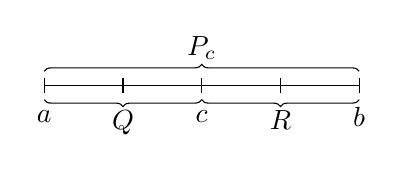
\begin{tikzpicture}
    		\draw (0,0) -- (4,0);
    		\foreach \pos/\descr in {0/a,1/,2/c,3/,4/b}
        	{
        		\draw (\pos,0) -- ++(0,1mm);
        		\draw (\pos,0) -- ++(0,-1mm);
        		\node[yshift=-4mm] at (\pos,0) {$\descr$};
        	}
    		\draw [underbrace] (0,0) -- node[below, yshift=-2mm]{$Q$} ++(2,0);
    		\draw [underbrace] (2,0) -- node[below, yshift=-2mm]{$R$} ++(2,0);
    		\draw [overbrace] (0,0) -- node[above, yshift=2mm]{$P_c$} ++(4,0);
		\end{tikzpicture}
		\end{center}

		By definition it's clear that
\[
\begin{aligned}
			U(f,P_c)&=U(f,Q)+U(f,R) \\ L(f,P_c)&=L(f,Q)+L(f,R).
		\end{aligned} \qquad (\ast)
\]
Hence
\[
\underbrace{U(f,P_c)-L(f,P_c)}_{<\varepsilon} = \underbrace{U(f,Q)-L(f,Q)}_{\geq 0}+\underbrace{U(f,R)-L(f,R)}_{\geq 0},
\]
therefore
\[
U(f,Q)-L(f,Q),\quad U(f,Q)-L(f,Q) < \varepsilon ,
\]
giving us $\left. f \right|_{[a,c]}$ and $\left. f \right|_{[c,b]}$ are integrable.
		\item[$\Leftarrow$:] We have that $\left. f \right|_{[a,c]}$ and $\left. f \right|_{[c,b]}$ are integrable. Then
\[
\forall \varepsilon >0, \exists Q,R : \left\{ \begin{aligned}
			U(f,Q)-L(f,Q) &< \frac{\varepsilon}2 \\ U(f,R)-L(f,R) &< \frac{\varepsilon}2
		\end{aligned} \right. \qquad (\ast\ast)
\]
where $Q,R$ are partitions of $[a,c],[c,b]$ respectively. Consider $P_c=Q\cup R$ (endpoints) and use $(\ast)$ and $(\ast\ast)$ to conclude.
	\end{itemize}

	We now establish additivity. We have
\[
\int_a^b f \leq U(f,P_c) = U(f,Q)+U(f,R) \leq L(f,Q)+L(f,R) + \varepsilon \leq \int_a^c f + \int_c^b f + \varepsilon
\]
and similarly
\[
\int_a^b f \geq \int_a^c f+\int_c^b f - \varepsilon .
\]
Since $\varepsilon$ is arbitrary, we conclude that
\[
\int_a^b f = \int_a^c f + \int_c^b f .
\]
\end{proof}

\begin{thm}
	$f:[a,b]\rightarrow \mathbb R$ is integrable. $\varphi: \mathbb R \rightarrow \mathbb R$ is continuous. Then $\varphi \circ f:[a,b]\rightarrow \mathbb R$ is integrable.
\end{thm}
\begin{proof}
	$f$ is integrable $\Rightarrow$ bounded, i.e. $\exists M>0:|f| \leq M$. So it's enough to consider $\varphi$ on closed bounded interval $[-M,M]$ which is continuous, meaning $\varphi$ is bounded, i.e. $\exists K>0:|\varphi|\leq K$ and $\varphi$ is uniformly continuous, which means
\[
\forall \overline\varepsilon >0, \exists \delta_{\overline\varepsilon} >0 : (x,y\in[-M,M],|x-y|<\delta_{\overline\varepsilon}) \Rightarrow |\varphi(x)-\varphi(y)|<\overline\varepsilon . \qquad (\ast)
\]
Also, $f$ is integrable, meaning
\[
\forall \eta >0, \exists Q_\eta \in \mathcal P=\{I_1,\ldots,I_n\} : U(f,Q_\eta)-L(f,Q_\eta) < \eta . \qquad (\ast\ast)
\]
We want to show that
\[
\forall \varepsilon >0, \exists P \in \mathcal P : U(\varphi \circ f, P)-L(\varphi \circ f,P) < \varepsilon .
\]
Take $P=Q_\eta$. Then
\[
U(\varphi \circ f, Q_\eta)-L(\varphi \circ f,Q_\eta) = \sum_{k=1}^{n} \left(\underbrace{ \underset{I_k}{\sup} \varphi \circ f - \underset{I_k}{\inf} \varphi \circ f}_{:=\underset{I_k}{\osc} \varphi \circ f} \right) \left|I_k\right| .
\]
The strategy is to break the sum into two parts: for the first sum we look at $k$'s such that $\underset{I_k}{\sup} f - \underset{I_k}{\inf} f < \delta_{\overline{\varepsilon}}$ which gives $\underset{I_k}{\sup} \varphi \circ f - \underset{I_k}{\inf} \varphi \circ f < \overline{\varepsilon}$ by uniform continuity of $\varphi$. For the second sum we look at $k$'s such that $\underset{I_k}{\sup} f - \underset{I_k}{\inf} f \geq \delta$, which there aren't many by $(\ast\ast)$ and bounded by $\eta$:
\[
\begin{aligned}\sum_{k:\underset{I_k}{\osc f}<\delta_{\overline{\varepsilon}}} \underset{I_k}{\osc} \varphi \circ f |I_k|+\sum_{k:\underset{I_k}{\osc f}\geq \delta_{\overline{\varepsilon}}} \underset{I_k}{\osc} \varphi \circ f |I_k| &\leq \overline{\varepsilon} \sum_{k=1}^n |I_k| +2K \sum_{k:\underset{I_k}{\osc f}\geq \delta_{\overline{\varepsilon}}} |I_k| \\ &=\overline{\varepsilon}(b-a) +\frac{2K}{\delta_{\overline{\varepsilon}}} \sum_{k:\underset{I_k}{\osc f}\geq \delta_{\overline{\varepsilon}}}\delta_{\overline{\varepsilon}} |I_k| \\ &\leq \overline{\varepsilon}(b-a) +\frac{2K}{\delta_{\overline{\varepsilon}}} \sum_{k:\underset{I_k}{\osc f}\geq \delta_{\overline{\varepsilon}}} \underset{I_k}{\osc} f |I_k| \\ &= \overline{\varepsilon}(b-a) +\frac{2K}{\delta_{\overline{\varepsilon}}}  \left(U(f,Q_\eta)-L(f,Q_\eta)\right) \\ &< \overline{\varepsilon}(b-a)+ \frac{2K \eta}{\delta_{\overline{\varepsilon}}} \end{aligned}
\]
where $\overline{\varepsilon},\eta$ are arbitrarily positively small. Choose $\overline{\varepsilon}=\frac{\varepsilon}{2(b-a)},\eta=\frac{\delta_{\overline{\varepsilon}}}{2K} \frac{\varepsilon}{2}$, then the above $=\frac{\varepsilon}{2}+\frac{\varepsilon}{2}=\varepsilon$.
\end{proof}

\begin{remark}
\begin{enumerate}
    \item A composition of two integrable functions is not necessarily integrable.
    \begin{example}
        Given $\varphi:\mathbb R \rightarrow \mathbb R$ and $f:[0,1]\rightarrow \mathbb R$ defined as follow,
\[
\varphi(x)=\left\{ \begin{aligned}
        &1 \quad x\neq 0 \\ &0\quad x=0
        \end{aligned} \right. , \qquad f(x)=\left\{ \begin{aligned}
        &\frac{1}{q} \quad x=\frac{p}{q}, p,q\in \mathbb N\text{ coprime} \\ &0\quad x=0\\&0\quad \text{otherwise}
        \end{aligned} \right.
\]
then
\[
\varphi \circ f (x)=\left\{ \begin{aligned}
            &1 \quad x\in \mathbb Q \cap (0,1] \\ &0 \quad \text{otherwise}
        \end{aligned} \right.
\]
which is not integrable.
    \end{example}
    \item What about $f\circ \varphi$ where $f$ is integrable and $\varphi$ continuous? Also not necessarily integrable. Counterexamples for this case are a bit harder to find.
\end{enumerate}
\end{remark}

\begin{thm}
$f,g:[a,b] \rightarrow \mathbb R$ integrable, then $f\cdot g$ is integrable. Moreover, if $g^{-1}$ is bounded, then $g^{-1}$ is integrable.
\end{thm}
\begin{proof}
$f$ is integrable means $f^2$ is also, since $\forall x\in[a,b]$, $f^2(x)=\varphi (f(x))$ where $\varphi:y\mapsto y^2$ on $\mathbb R$ which is continuous. We now write
\[
f\cdot g=\frac14 \left( (f+g)^2-(f-g)^2 \right)
\]
and by linearity of integration, $f\cdot g$ is integrable. If $g^{-1}$ is bounded, then $\exists \varepsilon >0 : |g(x)|\geq \varepsilon \ \forall x\in [a,b]$, and let
\[
\varphi(y)=\left\{\begin{aligned}
    \frac{1}{y} \quad &|y| \geq \varepsilon \\ \frac{y}{\varepsilon ^2} \quad &|y|<\varepsilon
\end{aligned} \right.
\]
\begin{center}
\begin{tikzpicture}
    \begin{axis}[axis x line=middle,axis y line=middle,
		xtick=\empty,ytick=\empty,
		xlabel={$y$},ylabel={$\varphi$},
		samples=1000,
		xmin=-2,xmax=2,
		ymin=-1.3,ymax=1.3]
    \addplot[domain=-1:1] {x};
    \addplot[domain=-2:-1] {1/x};
    \addplot[domain=1:2] {1/x};
    \end{axis}
\end{tikzpicture}
\end{center}

Then $\forall x\in [a,b]$, $\varphi(g(x))=\frac{1}{g(x)}$ where $g$ is integrable and $\varphi$ continuous, therefore $g^{-1}$ is integrable.
\end{proof}

\subsection{Fundamental theorem of calculus}
i.e. how to compute $\int_a^b f$?
\begin{thm}[FTC]
$f:[a,b]\rightarrow \mathbb R$ integrable, $F:[a,b]\rightarrow \mathbb R$ continuous and differentiable on $(a,b)$ such that $F'=f$. Then
\[
\int_a^b f(x) \ \mathrm d x = F(b)-F(a) .
\]
Also called Newton-Leibniz formula.
\end{thm}
\begin{proof}
It is enough to show that
\[
\forall P\in \mathcal P, L(f,P)\leq F(b)-F(a)\leq U(f,P) \qquad (\ast)
\]
since taking the sup and inf of $L$ and $U$ the equality still holds, which is now $L(f)\leq F(b)-F(a)\leq U(f)$, and since $f$ integrable, $L(f)=U(f)$ and therefore we have what we want to prove. So now let's prove $(\ast)$.

Let $P=\{I_1,\ldots,I_k\}$ where $I_k=[x_{k-1},x_k], 1\leq k\leq n$. Note that $\forall k$, $\forall c_k\in I_k$, $\underset{I_k}{\inf} f\leq f(c_k)\leq \underset{I_k}{\sup} f$, and since $F$ is continuous on $[x_{k-1},x_k]$ and differentiable on $(x_{k-1},x_k)$, by MVT
\[
\exists c_k\in (x_{k-1},x_k) : F(x_k)-F(x_{k-1})=F'(c_k)\cdot (x_k-x_{k-1})=f(c_k)\cdot (x_k-x_{k-1})
\]
and therefore
\[
\underset{I_k}{\inf} f |I_k|\leq F(x_k)-F(x_{k-1})\leq \underset{I_k}{\sup} f |I_k|
\]
and summing over all $k$'s gives us
\[
L(f,P)\leq \underbrace{\sum_k F(x_k)-F(x_{k-1})}_{\text{telescopic}}\leq U(f,P)
\]
and $(\ast)$ follows immediately.
\end{proof}
\begin{remark}
$f:[a,b]\rightarrow \mathbb R$ is integrable $\Rightarrow$ bounded. So FTC cannot be applied (yet) to unbounded functions, e.g.
\[
\int_0^1 \frac{1}{2\sqrt x} \ \mathrm d x = \left. \sqrt x \right|_0^1=1 .
\]
\end{remark}

\begin{remark}[Conventional generalisation]
If $b<a$,
\[
\int_a^b f := -\int_b^a f
\]
and
\[
\int_a^a f=0,
\]
which is consistent with additivity.
\end{remark}

\begin{thm}
Let $f:[a,b]\rightarrow \mathbb R$ be integrable, define $F:[a,b]\rightarrow \mathbb R, x\mapsto \int_a^x f$. Then $F\in \mathcal C [a,b]$. Moreover, if $x\in (a,b)$ and $f$ is continuous at $x$, $F'(x)=f(x)$.
\end{thm}
\begin{proof}
Let $x\in (a,b)$. $\forall h\in \mathbb R$ sufficiently small that $x+h\in [a,b]$, $F(x+h)-F(x)=\int_a^{x+h}f-\int_a^x f = \int_x^{x+h} f$ by additivity. $f$ is integrable implies that $\exists M>0: |f|\leq M$. Then
\[
|F(x+h)-F(x)|=\left|\int_x^{x+h}f\right|\leq \int_x^{x+|h|} |f|\leq M\int_x^{x+|h|}1=M|h|,
\]
i.e. $F$ is Lipschitz continuous, hence continuous. Checking left and right continuity at $x=b,a$ is left as an exercise. We now want to show that
\[
\lim_{h\rightarrow 0} \frac{F(x+h)-F(x)}{h}=f(x) ,
\]
i.e.
\[
\lim _{h\rightarrow 0} \left(\frac1h \int_x^{x+h}f(t) \ \mathrm d t - \underbrace{f(x)}_{\frac1h \int_x^{x+h}f(x) \ \mathrm d t}\right)=0 .
\]
But $f$ is continuous at $x$, i.e. $\forall \varepsilon >0, \exists \delta >0:|x-y|<\delta \Rightarrow |f(x)-f(y)|<\varepsilon$. Take $h:|h|<\delta$. Then
\[
\left|\frac{1}{h}\int_x^{x+h} \left(f(t)-f(x)\right) \ \mathrm d t \right|\leq \frac{1}{|h|} \int_x^{x+|h|} \underbrace{|f(t)-f(x)|}_{<\varepsilon \text{ as }|t-x|\leq |h|<\delta} \ \mathrm d t<\frac{1}{|h|}\varepsilon |h|=\varepsilon .
\]
Hence the desired result.
\end{proof}

\begin{thm}
Let $f:[a,b]\rightarrow \mathbb R$ be integrable. If $f$ is right-continuous at $a$,
\[
\lim_{h\rightarrow 0+} \frac1h \int_a^{a+h} f=f(a).
\]
Similarly, if $f$ left-continuous at $b$,
\[
\lim_{h\rightarrow 0+} \frac1h \int_{b-h}^b f=f(b).
\]
\end{thm}
\begin{proof}
$f$ is right-continuous at $a$ means $\forall \varepsilon >0, \exists \delta >0: 0<t-a<\delta \Rightarrow |f(t)-f(a)|<\varepsilon$. Let $h:|h|<\delta $. Then
\[
\begin{aligned}
    \left|\frac{1}{h}\int_a^{a+h}f-f(a) \right| &= \left|\frac{1}{h}\int_a^{a+h}f(t) \ \mathrm d t-\frac1h \int_a^{a+h} f(a) \ \mathrm d t \right| \\
    &\leq \frac{1}{|h|} \int_a^{a+|h|} |f(t)-f(a)| \ \mathrm d t \\
    &< \frac{1}{|h|}\varepsilon |h|=\varepsilon .
\end{aligned}
\]
The proof is similar for the second part.
\end{proof}
\begin{remark}
Theorem 1.3.2 and 1.3.3 together mean that $f$ is differentiable at any $x\in [a,b] : f$ is continuous at $x$.
\end{remark}
The definition of $\int_a^b f$ $\forall a,b\in \mathbb R$ allowed us to avoid looking at 1-sided limits for $x\in (a,b)$.
\begin{example}
Now we know $\forall p\geq 0$,
\[
\int_0^1 x^p = \int_0^1 \left( \frac{x^{p+1}}{p+1} \right)=\left. \frac{x^{p+1}}{p+1} \right|_0^1=\frac{1}{p+1},
\]
which is hard to do by hand.
\end{example}

\subsection{Methods of integration}
\begin{thm}[Integration by parts]
$f,g:[a,b]\rightarrow \mathbb R$ are continuous, differentiable on $(a,b)$ such that $f',g'$ are integrable. Then
\[
\int_a^b fg' = f(b)g(b)-f(a)g(a)-\int_a^b f'g .
\]
\end{thm}
\begin{proof}
$fg'$, $f'g$ and $(fg)'=f'g+fg'$ are all integrable as sums of products of integrable functions by Theorem 1.2.7. Then
\[
\begin{aligned}
    \int_a^b (fg)'&=f(b)g(b)-f(a)g(a) \qquad \text{by FTC}\\
    &=\int_a^b (f'g+fg') \qquad \text{by product rule} \\
    &=\int_a^b f'g + \int_a^b fg'\qquad \text{by linearity} .
\end{aligned}
\]
Rearranging gives desired result.
\end{proof}

\begin{example}
For any $a,b>0$,
\[
\begin{aligned}
    \int_a^b \log (x) \ \mathrm d x&=\int_a^b \log (x)\cdot x' \ \mathrm d x = \log (b)b-\log(a)a-\int_a^b \frac1x x \ \mathrm d x \\& = \log(b)b-\log(a)a-(b-a).
\end{aligned}
\]
\end{example}

\begin{thm}[Change of variables]
$f:[a,b]\rightarrow \mathbb R$ is differentiable such that $f'[a,b]\rightarrow \mathbb R$ is integrable, $g$ is continuous on image $f([a,b])$. Then
\[
\int_a^b g(f(x))f'(x) \ \mathrm d x = \int_{f(a)}^{f(b)}g(t) \ \mathrm d t .
\]
This is true even if $f(b)<f(a)$.
\end{thm}
\begin{proof}
For $x\in f([a,b])$, define
\[
G(x)=\int_{f(a)}^x g(t) \ \mathrm d t
\]
which is continuous at $x$, so $G$ is differentiable and $G'(x)=g(x)$ by Theorem 1.3.2. Chain rule gives
\[
\frac{\mathrm d}{\mathrm d x}G(f(x))=g(f(x))\cdot f'(x)
\]
hence
\[
\begin{aligned}
    \int_a^b g(f(x))\cdot f'(x) \ \mathrm d x &= \int_a^b G'(f(x)) \ \mathrm d x = G(f(b))-G(f(a)) \\ &= \int_{f(a)}^{f(b)} g(t) \ \mathrm d t - \int_{f(a)}^{f(a)} g(t) \ \mathrm d t \\ &= \int_{f(a)}^{f(b)} g(t) \ \mathrm d t .
\end{aligned}
\]
\end{proof}
\begin{example}
\[
\int_0^a e^{-\frac{x^2}{2}} x \ \mathrm d x=\int_0^a e^{-\frac{x^2}{2}} \left(\frac{x^2}{2}\right)' \ \mathrm d x .
\]
Let $g(t)=e^{-t},f(x)=\frac{x^2}{2}$. By theorem above the integral equals
\[
\int_0^{\frac{a^2}{2}} e^{-t} \ \mathrm d t=\left.-e^{-t}\right|_0^{\frac{a^2}{2}} = 1-e^{-\frac{a^2}{2}} .
\]
\end{example}
\begin{remark}[Consider integrals as functions of limits of integration]
In the proof of the theorem above we established that: if $f,h$ differentiable and $g$ continuous, we have
\[
\frac{\mathrm d}{\mathrm d x} \int_a^{f(x)}g(t) \ \mathrm d t=g(f(x))\cdot f'(x)
\]
by chain rule, and similarly
\[
\frac{\mathrm d}{\mathrm d x} \int_{h(x)}^a g(t) \ \mathrm d t=-\frac{\mathrm d}{\mathrm d x} \int_a^{h(x)} g(t) \ \mathrm d t=-g(h(x))\cdot h'(x).
\]
\end{remark}
\begin{example}[Construct solutions to certain PDEs]
Let $f:\mathbb R \rightarrow \mathbb R$ be continuous, $b:\mathbb R \times \mathbb R \rightarrow \mathbb R$ be differentiable, 
\[
u:\mathbb R\times \mathbb R \rightarrow \mathbb R, (x,t)\mapsto \int_{0}^{b(x,t)} f(s) \ \mathrm d s
\]
where $f$ continuous and $b$ differentiable. Now consider the partial derivative, we have
\[
\frac{\partial u(x,t)}{\partial x}=f(b(x,t))\cdot \frac{\partial b}{\partial x}(x,t)
\]
and
\[
\frac{\partial u(x,t)}{\partial t}=f(b(x,t))\cdot \frac{\partial b}{\partial t}(x,t)
\]
by chain rule. Take $b(x,t)=x-ct$ where $c\in \mathbb R$ is a parameter. Then
\[
\frac{\partial u(x,t)}{\partial x}+\frac1c \frac{\partial u(x,t)}{\partial t}=f(b(x,t))\cdot 1+\frac1c f(b(x,t))(-c)=0 ,
\]
i.e. a solution is found to the first-order linear PDE
\[
\frac{\partial u}{\partial x}+\frac1c \frac{\partial u}{\partial t}=0
\]
parameterised by $f\in \mathcal C(\mathbb R)$.
\end{example}

\begin{example}[Integrals can be used to define new functions]
The error function:
\[
\erf (x)=\frac{2}{\sqrt{\pi}} \int_0^x e^{-t^2} \ \mathrm d t,\quad x\in \mathbb R.
\]
where the integral is not computable, but FTC can be used to prove that $\erf$ is continuous. Or we could define $\log (0,\infty ) \rightarrow \mathbb R$ in the following way:
\[
x\mapsto \log (x)=\int_1^x \frac{1}{t} \ \mathrm d t
\]
which has properties\begin{itemize}
    \item well defined $\forall x>0$;
    \item
\[
\frac{\mathrm d}{\mathrm d x}\log (x)=\frac{\mathrm d}{\mathrm d x}\int_1^x \frac1t \ \mathrm d t = \frac1x .
\]
    \item
\[
\begin{aligned}\log x+\log y &= \int_1^x \frac1t \ \mathrm d t + \int_1^y \frac1t \ \mathrm d t \\ &=\int_1^x \frac1t \ \mathrm d t + \int_1^y \frac{1}{tx} x \ \mathrm d t\\&= \int_1^x \frac1t \ \mathrm d t + \int_x^{xy}\frac1s \ \mathrm d s \qquad \text{change of variable: }s(t)=xt \\&= \int_1^{xy} \frac1t \ \mathrm d t \\&= \log (xy), \end{aligned}
\]
which, as we've seen, was difficult to prove using power series definition of log.
\end{itemize}
\end{example}

\section{Improper integrals}
\begin{defn}
Let $f:(a,b]\rightarrow \mathbb R$ be such that $f$ is Riemann integrable on $[c,b] \ \forall c\in (a,b]$. Then
\[
\underbrace{\int_a^b f}_{\text{Improper}}:=\lim_{\underbrace{\varepsilon \downarrow 0}_{\varepsilon \rightarrow 0+}} \underbrace{\int_{a+\varepsilon}^b f}_{\text{Riemann}},
\]
which is a serious generalisation: $f$ can be unbounded. If the limit exists and is finite, we say $\int_a^b f$ converges. Otherwise $\int_a^b f$ diverges.

Similarly, if $f:[a,b)\rightarrow \mathbb R$ is such that $f$ is Riemann integrable on $[a,c] \ \forall c\in [a,b)$, then
\[
\int_a^b f := \lim_{\varepsilon \downarrow 0} \int_a^{b-\varepsilon} f .
\]
\end{defn}
\begin{example}
Let $p>-1$, then
\[
\begin{aligned}
    \int_0^1 x^p \ \mathrm d x &=\lim_{\varepsilon \downarrow 0} \int_\varepsilon^1 x^p \ \mathrm d x=\lim_{\varepsilon \downarrow 0} \left. \frac{x^{p+1}}{p+1} \right|_\varepsilon^1 \\
    &=\lim_{\varepsilon \downarrow 0} \left(\frac{1}{p+1}-\underbrace{\frac{\varepsilon^{p+1}}{p+1}}_{\rightarrow 0\text{ since }p+1>0} \right) \\&= \frac{1}{p+1}.
\end{aligned}
\]
So $\int_0^1 x^p \ \mathrm d x<\infty$ for $p>-1$, i.e. it converges. If $p=1$,
\[
\int_0^1 \frac{1}{x} \ \mathrm d x = \lim_{\varepsilon \downarrow 0} \left. \log x \right|_\varepsilon^1 = \lim_{\varepsilon \downarrow 0} \left(-\log(\varepsilon)\right) = +\infty,
\]
so it diverges.
\end{example}
\begin{remark}
If $p\geq 0$ we get the same answer: if $f$ is integrable on $[a,b]$, then
\[
\underbrace{\int_a^b f}_{\text{improper}} = \underbrace{\int_a^b f}_{\text{Riemann}}
\]
by continuity, i.e. the two definitions are consistent.
\end{remark}

\begin{defn}
Let $c\in (a,b)$ and $f:[a,b]\backslash\{c\} \rightarrow \mathbb R$ be Riemann integrable on $[a,c-\delta]$ and $[c+\varepsilon ,b]$ for all $\delta>0,\varepsilon>0$ small enough.
\begin{center}
\begin{tikzpicture}
    \begin{axis}[axis x line=middle,axis y line=middle,
		xtick=\empty,ytick=\empty,
		xlabel={$x$},ylabel={$y$},
		samples=1000,
		xmin=-1,xmax=7,
		ymin=-0.5,ymax=45,
		xtick = {1,2,3},
		xticklabels = {$a$,$c$,$b$}]
    \addplot[domain=-1:1.9] {1/(0.5*x-1)^2};
    \addplot[domain=2.1:5] {1/(0.5*x-1)^2};
    \end{axis}
\end{tikzpicture}
\end{center}
Then
\[
\int_a^b f := \underbrace{\int_a^c f}_{\text{improper}} + \underbrace{\int_c^b f}_{\text{improper}} = \lim_{\delta \downarrow 0}\int_a^{c-\delta} f+\lim_{\varepsilon \downarrow 0}\int_{c+\varepsilon}^{b} f
\]
\textbf{NB} $\delta,\varepsilon$ are taken to $0$ independently.
\end{defn}
\subsection{Unbounded intervals}
\begin{defn}
$f:[a,\infty) \rightarrow \mathbb R$ such that $f$ is integrable on $[a,b] \ \forall b\geq a$. Then
\[
\int_a^\infty f := \lim_{b\uparrow \infty} \int_a^b f
\]
and similarly if $f$ is integrable on $[b,a] \ \forall b\leq a$
\[
\int_{-\infty}^a f := \lim_{b\downarrow -\infty} \int_b^a f
\]
and
\[
\int_{-\infty}^\infty f:= \underbrace{\int_{-\infty}^c f + \int_c^{\infty} f}_{\text{improper integrals defined above}}=\lim_{R_1 \rightarrow -\infty} \int_{R_1}^c f + \lim_{R_2 \rightarrow +\infty} \int_c^{R_2} f .
\]
where $c\in \mathbb R$ any fixed constant.

\textbf{NB} $R_1\rightarrow -\infty, R_2\rightarrow +\infty$ independently.
\end{defn}
\begin{example}
\[
\int_{-\infty}^\infty x^3 \ \mathrm d x
\]
doesn't exist. But
\[
\lim_{R\rightarrow \infty} \int_{-R}^R x^3 \ \mathrm d x=0
\]
and moreover, we can let $R_2$ be some function $R_1$ and right hand side can be whichever real number we want.
\end{example}

Exercise: check the RHS of the last definition does not depend on $c$.
\begin{remark}[Warnings]
\begin{itemize}
    \item The space of improperly integrable functions is a linear space, but not an algebra (in the sense that $f,g$ improperly integrable $\not\Rightarrow$ $f\cdot g$ is integrable). e.g.
\[
f(x)=g(x)=\frac{1}{\sqrt{x}}, \quad x\in (0,1]
\]
are properly integrable since $p=\frac12<1$, but $x\mapsto \frac1x$ is not.
    \item Similarly, $\varphi$ is continuous and $f$ is improperly integrable $\not\Rightarrow$ $\varphi \circ f$ is improperly integrable. e.g.
\[
\varphi : y\mapsto y^2,\ f:x\mapsto \frac{1}{\sqrt{x}},\quad x\in (0,1].
\]
Then $\varphi (f(x))=\frac{1}{x}$ which is again not integrable.
    \item $f$ is improperly integrable $\not\Rightarrow$ $|f|$ is improperly integrable. See notes and assignments.
\end{itemize}
\end{remark}

\begin{thm}[Absolute comparison test]
Let $f:[a,\infty)\rightarrow \mathbb R$ be Riemann integrable on $[a,b] \ \forall b\geq a$. Suppose
\[
\int_a^\infty |f|<\infty .
\]
Then
\[
\int_a^\infty f < \infty .
\]
In this case we say $\int_a^\infty f$ is absolutely convergent.

More generally, if there's a function $g:[a,\infty)\rightarrow[0,\infty)$ such that $|f|\leq g$, then
\[
\int_0^\infty g <\infty \Rightarrow \int_a^\infty f <\infty.
\]
\end{thm}

\begin{remark}
\begin{enumerate}
    \item Compare this with the $M$-test for infinite series
    \item Similar statements apply to improper integral of $f:[a,b]\backslash \{c\}\rightarrow \mathbb R$ where $c\in [a,b]$ which is not necessarily bounded
\end{enumerate}
\end{remark}
\begin{proof}
By Cauchy criterion, convergence of integral of $|f|$ implies that
\[
\forall \varepsilon >0, \exists L_\varepsilon : L_2>L_1>L_\varepsilon \Rightarrow \left| \int_a^{L_2} |f|-\int_a^{L_1} |f| \right|<\varepsilon .
\]
But by additivity
\[
\left| \int_a^{L_2} |f|-\int_a^{L_1} |f| \right|=\left|\int_{L_1}^{L_2} |f| \right|=\int_{L_1}^{L_2} |f| .
\]
So
\[
\left|\int_{L_1}^{L_2} f \right|\leq\int_{L_1}^{L_2} |f|<\varepsilon .
\]
Therefore
\[
\int_a^\infty f <\infty
\]
by the reverse Cauchy criterion.

For the second part, repeat the above steps, simply replacing $f$ with $|f|$ and $|f|$ with $g$.
\end{proof}

\begin{example}
Does
\[
\int_0^\infty \frac{\cos x^2}{1+x^{1+\varepsilon}} \ \mathrm d x
\]
converge $\forall \varepsilon >0$? We can't get rid of the $1+$ in denominator since that would give a divergence, therefore we break it into two parts using additivity:
\[
\underbrace{\int_0^1 \frac{\cos x^2}{1+x^{\varepsilon +1}} \ \mathrm d x}_{\text{Riemann integrable, so no need to worry}}+\int_1^\infty \frac{\cos x^2}{1+x^{\varepsilon +1}} \ \mathrm d x
\]
and for the second part we have
\[
\begin{aligned}
\left| \int_1^\infty \frac{\cos x^2}{1+x^{\varepsilon +1}} \ \mathrm d x\right| &\leq \int_1^\infty \left| \frac{\cos x^2}{1+x^{1+\varepsilon}} \ \mathrm d x \right| = \int_1^\infty \overbrace{\frac{|\cos x^2|}{1+x^{1+\varepsilon}}}^{\text{the }|f|\text{ in the theorem}} \ \mathrm d x \\
&\leq \int_1^\infty \frac{1}{1+x^{1+\varepsilon}} \ \mathrm d x \leq \int_1^\infty \frac{1}{x^{1+\varepsilon}} \ \mathrm d x
\end{aligned}
\]
and the last integral can be computed analytically:
\[
\left. -\frac{1}{\varepsilon} x^{-\varepsilon} \right|_1^\infty = \frac{1}{\varepsilon} < \infty.
\]
We conclude the desired result.
\end{example}

\section{Sequences and series of functions}
Main task: justify the interchange of maths operations.
\begin{example}
\[
\lim_{x\rightarrow c} \lim_{n\rightarrow \infty} f_n(x)\overset{?}{=} \lim_{n\rightarrow \infty}\lim_{x\rightarrow c} f_n(x)
\]
\[
\lim_{n\rightarrow \infty} \int_a^b f_n(x) \ \mathrm d x \overset{?}{=} \int_a^b \lim_{n\rightarrow \infty} f_n(x) \ \mathrm d x
\]
\[
\left(\sum_{n=1}^\infty f_n(x) \right)' \overset{?}{=} \sum_{n=1}^\infty f_n'(x)
\]
\end{example}

\subsection{Pointwise and uniform convergence}
Let $f_n:\Omega \rightarrow \mathbb R, n\geq 1$ be a sequence of functions on $\Omega \subset \mathbb R$ (not necessarily closed bounded).
\begin{defn}[Pointwise convergence]
$(f_n)_{n\geq 1}$ on $\Omega$ converges to $f:\Omega \rightarrow \mathbb R$ \textit{pointwise} if
\[
\forall x\in\Omega, \lim_{n\rightarrow \infty} f_n(x)=f(x) .
\]
\end{defn}
\begin{notation}
    $f_n \rightarrow f$.
\end{notation}
\begin{remark}
Pointwise convergence is often not enough to justify various interchanges. [If all you know is pointwise convergence, you do not know much.]
\end{remark}
So sit tight for incoming examples of bad news!

\begin{example}
$f_n:[0,1]\rightarrow \mathbb R, x\mapsto x^{\frac1n}$.
\begin{center}
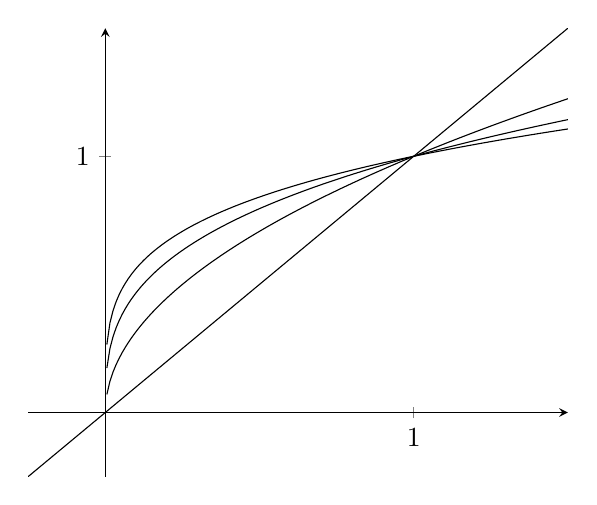
\begin{tikzpicture}
\begin{axis}[axis x line=middle,axis y line=middle,
		xtick=1,ytick=1,
		samples=1000,
		xmin=-0.25,xmax=1.5,
		ymin=-0.25,ymax=1.5]
\addplot[]{x};
\addplot[]{x^0.5};
\addplot[]{x^0.33};
\addplot[]{x^0.25};
\end{axis}
\end{tikzpicture}
\end{center}
We know $f_n(0)=0 \ \forall n$, and for $x\in(0,1]$, $x^{1/n}=e^{\log x^{1/n}} = e^{\frac1n \log x} \rightarrow e^0 =1$. So $f_n \rightarrow f=\left\{\begin{aligned}&0\qquad x=0\\&1\qquad \text{otherwise}\end{aligned} \right.$ which is not continuous. [Pointwise convergence doesn't preserve continuity!]

So
\[
\lim_{x\rightarrow 0+}\lim_{n\rightarrow \infty} f_n(x)=\lim_{x\rightarrow 0+} 1 = 1
\]
but
\[
\lim_{n\rightarrow \infty} \lim_{x\rightarrow 0+} f_n(x)=\lim_{n\rightarrow \infty} 0 = 0.
\]
\end{example}

\begin{example}
Pointwise can be very non-uniform. Let
\[
f_n(x)=\left\{\begin{aligned}
&2nx\qquad &0\leq x\leq \frac{1}{2n} \\ &-2n\left(x-\frac1n \right)\qquad &\frac{1}{2n}< x \leq \frac1n \\ &0\qquad &x>\frac1n
\end{aligned} \right.
\]
\begin{center}
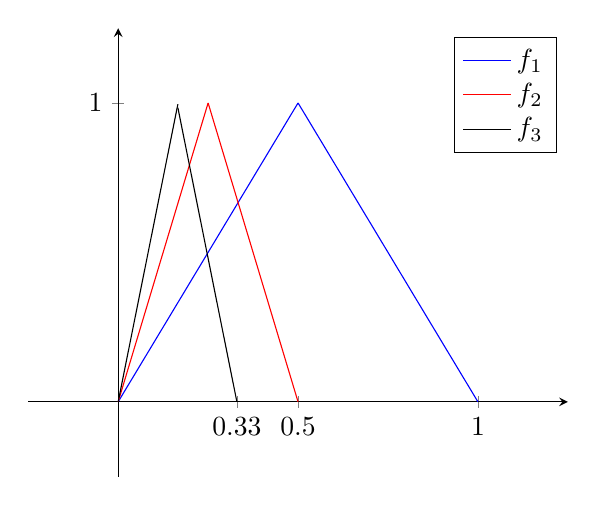
\begin{tikzpicture}
\begin{axis}[axis x line=middle,axis y line=middle,
		xtick={1,0.5,0.33},ytick=1,
		samples=1000,
		xmin=-0.25,xmax=1.25,
		ymin=-0.25,ymax=1.25]
\addplot[domain=0:0.5,blue]{2*x};
\addplot[domain=0.5:1,blue]{-2*(x-1)};
\addplot[domain=0:0.25,red]{4*x};
\addplot[domain=0.25:0.5,red]{-4*(x-0.5)};
\addplot[domain=0:0.166]{6*x};
\addplot[domain=0.166:0.33]{-6*(x-0.33)};
\legend{$f_1$,,$f_2$,,$f_3$}
\end{axis}
\end{tikzpicture}
\end{center}
We claim that $f_n\rightarrow 0$. We know $f_n(0)=0 \ \forall n \Rightarrow f(0)=0$, but also
\[
\forall x>0, f_n(x)=0 \ \forall n: \frac1n <x .
\]
However
\[
\underset{x\in [0,1]}{\sup} |f_n(x)-0|=1\quad \forall n\in \mathbb N
\]
which is constant and doesn't even depend on $x$! Even worse, define
\[
w_n=nf_n\qquad \text{(Witch's hat)}
\]
Then $w_n\rightarrow 0$ still but
\[
\underset{x\in [0,1]}{\sup} |w_n(x)-0|=n
\]
which goes to $\infty$! Pointwise convergence loses all its significance here.
\end{example}

\begin{example}
Let
\[
f_n:\mathbb R\rightarrow \mathbb R, x\mapsto \underbrace{\mathcal X_{[n,n+1]}(x)}_{\text{Indicator function}}.
\]
Then
\[
\lim_{n\rightarrow \infty} \mathcal X_{[n,n+1]}(x)=0 \quad \forall x\in \mathbb R ,
\]
i.e. $\mathcal X_{[n,n+1]} \rightarrow 0$. What happens to the improper integral?
\[
\lim_{n\rightarrow \infty} \int_{-\infty}^\infty \mathcal X_{[n,n+1]}=\lim_{n\rightarrow \infty} 1\times 1 = 1
\]
but
\[
\int_{-\infty}^\infty \lim_{n\rightarrow \infty} \mathcal X_{[n,n+1]}=\int_{-\infty}^\infty 0=0.
\]
\end{example}

\begin{example}
$f_n:x\mapsto \sin (nx)$ on $\mathbb R,\ n\in \mathbb N$. Take $\displaystyle x=\frac{p}{q}\pi,\ 0<p<q$, i.e. rational multiple of $\pi$. Then $\sin ((kq)x)=\sin(pk\pi)=0$ and $\sin((2kq+1)x) = \sin x >0$ which converge to different limits. So we claim $(f_n) \not\rightarrow .$ (Doesn't converge pointwise)

However for any $f\in [a,b]$-Riemann integrable,
\[
\lim_{n\rightarrow \infty} \int_a^b f(x) \sin (nx) \ \mathrm d x =0
\]
(Riemann-Lebesgue Lemma).
\end{example}

\begin{example}
Let $g_n(x):=\frac{\sin n x}{n},\ x\in \mathbb R$. Then $|g_n(x)|\leq \frac{1}{n} \rightarrow 0$. So $g_n\rightarrow 0$. Unlike the Witch's hat, even $\underset{\mathbb R}{\sup}|g_n|\rightarrow 0$. But
\[
\left(\lim_{n\rightarrow \infty}g_n\right)'\neq \lim_{n\rightarrow \infty} g_n' = \lim_{n\rightarrow \infty} \cos n x
\]
which doesn't exist.
\end{example}

\begin{example}
$(f_n):[0,1]\rightarrow \mathbb R$ defined in following way:
\[
\begin{aligned}f_0=\mathcal X_{[0,1]},\\f_1=\mathcal X_{\left[0,\frac12\right]},f_2=\mathcal X_{\left[\frac12,1\right]},\\f_3=\mathcal X_{\left[0,\frac14\right]},f_4=\mathcal X_{\left[\frac14,\frac12\right]},f_5=\mathcal X_{\left[\frac12,\frac34\right]},f_6=\mathcal X_{\left[\frac34,1\right]},\\ \cdots\end{aligned}
\]
Note that $f_n \not\rightarrow$ as $\forall x\in [0,1], \ f_n(x)$ contains infinitely many 0's and 1's. However $\int_0^1 f_n \rightarrow 0$ since $\sup f=1$ constantly but the size of subintervals goes to 0.
\end{example}

\begin{defn}[Uniform convergence]
A sequence $f_n:\Omega \rightarrow \mathbb R,\ n\geq 1$ \textit{uniformly converges} to $f:\Omega \rightarrow \mathbb R$ if
\[
\forall \varepsilon >0,\ \exists \delta N_\varepsilon : n>N_\varepsilon \Rightarrow |f_n(x)-f(x)|<\varepsilon \ \forall x\in \Omega.
\]
\end{defn}
\begin{notation}
\begin{itemize}
    \item $f_n \rightrightarrows f$.
    \item $f_n \not\rightrightarrows$ means $f_n$ does not converge uniformly.
    \item $\|f_n\|_{\infty} = \underset{\Omega}{\sup} |f_n|$. Left-hand side is called sup norm of $f_n$.
\end{itemize}
\end{notation}
So $f_n \rightrightarrows f$ means that $\forall \varepsilon >0,\ \exists N_\varepsilon : n>N_\varepsilon \Rightarrow \|f-f_n\|_{\infty}<\varepsilon$ or even simpler
\[
\lim_{n \rightarrow \infty} \|f-f_n\|_{\infty} =0 .
\]
Note that in this language, pointwise convergence can be written as
\[
\lim_{n\rightarrow \infty} |f_n(x)-f(x)|=0 \ \forall x\in \Omega .
\]
\begin{prop}
$(f_n \rightrightarrows f) \underset{\not\Leftarrow}{\Rightarrow} (f_n\rightarrow f)$
\end{prop}
This is trivial.
\begin{defn}
A sequence $(f_n)$ on $\Omega \subset \mathbb R$ is \textit{uniformly Cauchy} if
\[
\forall \varepsilon >0,\ \exists N_\varepsilon : n,m>N_\varepsilon \Rightarrow \|f_n-f_m\|_\infty < \varepsilon .
\]
\end{defn}
\begin{thm}
$f_n \rightrightarrows$ on $\Omega \Leftrightarrow (f_n)$ is uniformly Cauchy.
\end{thm}
\begin{proof}
\begin{itemize}
    \item[$\Rightarrow$:] Let $f:\Omega \rightarrow \mathbb R$ be the limit, i.e.
\[
\forall \varepsilon, \ \exists N_\varepsilon : n>N_\varepsilon \Rightarrow \|f_n-f\|_\infty < \frac{\varepsilon}{2} .
\]
Take any $n,m>N_\varepsilon$,
\[
\begin{aligned}\|f_n-f_m\|_\infty &= \underset{\Omega}{\sup} |f_n-f_m| =\underset{\Omega}{\sup} |f_n-f+f-f_m|\\&\leq \underset{\Omega}{\sup} (|f_n-f|+|f_m-f|) \qquad \text{triangle inequality} \\&\leq \underset{\Omega}{\sup}|f_n-f|+\underset{\Omega}{\sup}|f_m-f|=\|f_n-f\|_\infty+\|f_m-f\|_\infty \\&<\frac{\varepsilon}{2}+\frac{\varepsilon}{2}=\varepsilon .\end{aligned}
\]
    
    [We also proved triangle inequality for $\|\cdot \|_\infty$. Justified terminology!]
    \item[$\Leftarrow$:] We have $\forall \varepsilon, \ \exists N_\varepsilon : n,m>N_\varepsilon \Rightarrow \underset{\Omega}{\sup} |f_n-f_m|<\varepsilon .$ But $|f_n-f_m|\leq \underset{\Omega}{\sup} |f_n-f_m| \ \forall x\in \Omega$ by definition, so $(f_m(x))$ is Cauchy, so it converges to $f(x)$ for some $f:\Omega \rightarrow \mathbb R$, i.e. $f_m\rightarrow f$ pointwise. We then write $\forall n,m >N_\varepsilon$,
\[
f_m-\varepsilon \leq f_n \leq f_m+\varepsilon \text{on }\Omega
\]
(this is just rewriting the hypothesis of being Cauchy), then take $\lim_{m\rightarrow \infty}$ we have
\[
f-\varepsilon \leq f_n \leq f+\varepsilon
\]
so $|f_n-f|<\varepsilon \ \forall x\in \Omega$ i.e. $f_n\rightrightarrows f$.
\end{itemize}
\end{proof}

\begin{remark}
$\|\cdot\|_\infty$ is a norm on the space of bounded functions on $\Omega$, denoted $\mathcal B(\Omega)$. Notion of a norm means that $\|\cdot\|:B(\Omega)\rightarrow \mathbb R$ has following properties:
\begin{enumerate}
    \item $\|f\|_\infty \geq 0 \ \forall f\in B(\Omega)$
    \item $\|\lambda f\|_\infty = |\lambda|\|f\|_\infty \ \forall \lambda \in \mathbb R$
    \item $\forall f,g\in B(\Omega)$, $\|f+g\|_\infty \leq \|f\|_\infty+\|g\|_\infty$
\end{enumerate}
\end{remark}

\begin{thm}[Uniform continuity preserves continuity]
A sequence of continuous functions $(f_n):\Omega \rightarrow \mathbb R,\ n\geq 1$ converges uniformly to $f:\Omega \rightarrow \mathbb R$. Then $f$ is continuous on $\Omega$.
\end{thm}
\begin{proof}
$f_n\rightrightarrows f$ means \begin{equation}\forall \varepsilon >0, \ \exists N_\varepsilon : n>N_\varepsilon \Rightarrow \|f_n-f\|_\infty < \frac{\varepsilon}{3} .\end{equation} Also $f_n$ is continuous at $x_0\in \Omega$, meaning \begin{equation}\forall \varepsilon >0, \ \exists \delta_\varepsilon >0 : |x-x_0|<\delta_\varepsilon^{(n)} \Rightarrow |f_n(x)-f_n(x_0)|<\frac{\varepsilon}{3} .\end{equation} Fix any $n>N_\varepsilon$ and $\delta_\varepsilon^{(n)} >0$. Then
\[
\begin{aligned}|f(x)-f(x_0)|&=|f(x)-f_n(x)+f_n(x)-f_n(x_0)+f_n(x_0)-f(x_0)|\\&\leq \underbrace{|f(x)-f_n(x)|}_{<\frac{\varepsilon}{3}\text{ by (1)}}+\underbrace{|f_n(x)-f_n(x_0)|}_{<\frac{\varepsilon}{3}\text{ by (2)}}+\underbrace{|f_n(x_0)-f(x_0)|}_{<\frac{\varepsilon}{3}\text{ by (1)}} \\ &<3\cdot \frac{\varepsilon}{3}=\varepsilon\end{aligned}
\]
\end{proof}
\begin{notation}
$\mathcal C_b (\Omega, \|\cdot\|_\infty)$ is a linear space of continuous, bounded functions on $\Omega$, equipped with $\|\cdot \|_\infty$ norm. ($\infty$-dim normed space)
\end{notation}
\begin{thm}[Completeness]
$\mathcal C_b (\Omega, \|\cdot\|_\infty)$ is a complete normed space, i.e. any Cauchy sequence $(f_n)\subset \mathcal C_b(\Omega)$ converges to some $f\in \mathcal C_b (\Omega)$.

Without using all the jargon: a uniformly Cauchy sequence of continuous bounded functions converges to a continuous and bounded function.
\end{thm}
\begin{remark}
A Cauchy sequence $(a_n)\subset \underbrace{(V,\|\cdot\|)}_{\text{normed space}}$ is such that
\[
\forall \varepsilon >0,\ \exists N_\varepsilon : n,m>N_\varepsilon \Rightarrow \|a_n-a_m\|<\varepsilon .
\]
This definition ensures that the two formulated versions of Theorem 3.1.13 are equivalent.
\end{remark}
\begin{proof}
$f_n \rightrightarrows f$ and $f_n$ is continuous $\forall n$, so by Theorem 3.1.12 $f$ is continuous.

We can pick $n:\|f-f_n\|_\infty \leq 1$. Then
\[
\|f\|_\infty \|f_n+f-f_n\|_\infty \leq \|f_n\|_\infty+\|f-f_n\|_\infty <\infty+1=\infty .
\]
Therefore $f$ is also bounded.
\end{proof}

\begin{example}
$f_n=\frac{1}{2n} \mathcal X_{[-n,n]}$ on $\mathbb R$. Then $\|f_n\|_\infty = \frac{1}{2n} \rightarrow 0$. So $f_n \rightrightarrows 0$. And $\int_{-\infty}^\infty f_n=1\neq \int_{-\infty}^\infty \lim_{n\rightarrow \infty} f_n$. But good news is on bounded interval this inequality does not occur.
\end{example}
\begin{thm}
$f_n:[a,b]\rightarrow \mathbb R$ is integrable $\forall n$ and $f_n \rightrightarrows f:[a,b]\rightarrow \mathbb R$. Then $f$ is integrable and $\int_a^b f_n \rightarrow \int_a^b f$. (i.e.
\[
\lim_{n\rightarrow \infty} \int_a^b f_n = \int_a^b \lim_{n\rightarrow \infty} f_n,
\]
limit and integral is interchangeable in this case.)
\end{thm}
\begin{proof}
Uniform convergence means
\[
\forall \varepsilon >0,\ \exists N_\varepsilon : n>N_\varepsilon \Rightarrow \|f-f_n\|_\infty < \frac{\varepsilon}{4(b-a)} .
\]
Integrability $\forall n$ means
\[
\forall \varepsilon >0,\ \exists P_n \in \mathcal P : U(f_n,P_n)-L(f_n,P_n)<\frac{\varepsilon}2 ,
\]
where we let $P_n=\{I_1,\ldots,I_m\}$. Fix $n>N_\varepsilon$. Then
\[
U(f_n,P_n)-L(f_n,P_n)=\sum_{k=1}^m \left(\underset{I_k}{\sup} f-\underset{I_k}{\inf} f \right) |I_k|.
\]
Side computation:
\[
\begin{aligned}
    \underset{I_k}{\sup} f &= \underset{I_k}{\sup} (f_n+f-f_n)\\&\leq \underset{I_k}{\sup} f_n+\underset{I_k}{\sup} (f-f_n)\\&\leq \underset{I_k}{\sup} f_n + \underset{I_k}{\sup} |f-f_n|\\&\leq \underset{I_k}{\sup} f_n+\|f-f_n\|_\infty .
\end{aligned}
\]
Similarly we can get a lower bound for $\underset{I_k}{\inf} f$, namely $\underset{I_k}{\inf} f_n-\|f-f_n\|_\infty .$ So
\[
\begin{aligned}\sum_{k=1}^m \left(\underset{I_k}{\sup} f-\underset{I_k}{\inf} f \right) |I_k| &\leq \underbrace{\sum_{k=1}^m \left(\underset{I_k}{\sup} f_n-\underset{I_k}{\inf} f_n \right) |I_k|}_{<\frac{\varepsilon}{2} \text{ by integrability}}+2\sum_{i=1}^m \underbrace{\|f-f_n\|_\infty}_{<\frac{\varepsilon}{4(b-a)} \text{ by uniform convergence}} |I_k| \\&< \frac{\varepsilon}{2}+2\frac{\varepsilon}{4(b-a)}(b-a)=\varepsilon ,\end{aligned}
\]
which implies integrability of $f$.

Now
\[
\begin{aligned}\left| \int_a^b f_n - \int_a^b f \right| &\leq \int_a^b |f_n-f| \\& \leq \int_a^b \|f_n-f\|_\infty \qquad \text{this is why we need bounded} \\&= \underbrace{\|f_n-f\|_\infty}_{\rightarrow 0} (b-a) .\end{aligned}
\]
So $\int_a^b f_n \rightarrow \int_a^b f$.
\end{proof}

\subsection{Functions of 2 variables}
\begin{defn}
$f:\Omega \subset \mathbb R^2 \rightarrow \mathbb R$ is \textit{continuous} at $x\in \Omega$ if
\[
\forall \varepsilon >0,\ \exists \delta(\varepsilon ,x)>0: (y\in \Omega,\ \underbrace{|x-y|}_{\text{Euclidean distance}}<\delta ) \Rightarrow \underbrace{|f(x)-f(y)|}_{\text{absolute value}}<\varepsilon .
\]
\end{defn}
This is the same with previous definition of continuity, only 2-variable.
\begin{defn}
$f:\Omega \subset \mathbb R^2 \rightarrow \mathbb R$ is \textit{uniformly continuous} on $\Omega$ if
\[
\forall \varepsilon >0,\ \exists \delta_\varepsilon : (x,y\in \Omega: |x-y|<\delta_\varepsilon) \Rightarrow |f(x)-f(y)|<\varepsilon .
\]
\end{defn}
This is the same with Definition 1.1.13.
\begin{thm}
$\Omega \subset \mathbb R^2$ closed and bounded. If $f:\Omega \rightarrow \mathbb R$ is continuous then it's uniformly continuous.
\end{thm}
\begin{proof}[Hint for proof]
Use Bolzano-Weierstrass theorem for bounded sequences in $\mathbb R^2$. (Similar to proof of Theorem 1.1.14.)
\end{proof}
\begin{thm}
Let $f:[a,b]\times [c,d]\rightarrow \mathbb R$ be continuous. Define $I:[c,d] \rightarrow \mathbb R$, $t\mapsto \int_a^b  f(x,t) \ \mathrm d x.$ Then $I$ is continuous on $[c,d]$.
\end{thm}
\begin{proof}
We know $[a,b]\times [c,d]$ is closed and bounded. Then $f$ is uniformly continuous. Fix any $t_0\in [c,d]$. Then
\[
|I(t)-I(t_0)|\leq \int_a^b |f(x,t)-f(x,t_0)| \ \mathrm d x .
\]
Uniform continuity means $\forall \varepsilon >0,\ \exists \delta_\varepsilon >0 : $
\[
(|(x,t)-(x_0,t_0)|<\delta_\varepsilon, (x,t),(x_0,t_0)\in [a,b]\times [c,d])\Rightarrow |f(x,t)-f(x_0,t_0)| <\frac{\varepsilon}{b-a} .
\]
Now pick any $t:|t-t_0|<\delta_\varepsilon$. Then $|(x,t_0)-(x,t)|<\delta_\varepsilon$. So
\[
|I(t)-I(t_0)| < \int_a^b \frac{\varepsilon}{b-a}=\varepsilon,
\]
i.e. $I$ is continuous at $t_0$ by definition.
\end{proof}

\begin{thm}
$f,\frac{\partial f}{\partial t}:[a,b]\times [c,d]\rightarrow \mathbb R$ are continuous. Then $t\mapsto \int_a^b f(x,t) \ \mathrm d x$ is differentiable on $[c,d]$ and
\[
\frac{\partial}{\partial t} \int_a^b f(x,t) \ \mathrm d x = \int_a^b \frac{\partial }{\partial t} f(x,t) \ \mathrm d x .
\]
\end{thm}
\begin{proof}
Define
\[
F(t):=\int_a^b f(x,t) \ \mathrm d x
\]
and
\[
G(t) := \int_a^b \frac{\partial f}{\partial t} (x) \ \mathrm d x.
\]
We would like to show that $F$ is differentiable on $(c,d)$ and $F'=G$.

We write
\[
\left| \frac{F(t+h)-F(t)}{h}-G(t) \right|\mathrm dx = \left| \int_a^b \frac{f(x,t+h)-f(x,t)}{h}-G(t) \right|\mathrm  dx
\]
and since $f(x,\cdot)$ is continuous and differentiable on $[c,d]$, we can apply MVT and the above is
\[
\left| \int_a^b \frac{\partial f}{\partial t} (x,\tau) - \frac{\partial f}{\partial t} (x,t) \right|\mathrm d x
\]
for some $\tau \in [t,t+h]$. But $\frac{\partial f}{\partial t}$ is continuous on closed bounded interval $[a,b]\times [c,d]$, so we have uniform continuity. Therefore $\forall \varepsilon >0,\ \exists \delta_\varepsilon :$
\[
|\tau -t|<\delta_\varepsilon \Rightarrow \left| \frac{\partial f}{\partial t} (x,\tau) - \frac{\partial f}{\partial t} (x,t) \right| < \frac{\varepsilon}{b-a} .
\]
So pick $|h|<\delta_\varepsilon$, we have
\[
\left| \frac{F(t+h)-F(t)}{h}-G(t) \right|\mathrm dx<\int_a^b \frac{\varepsilon}{b-a} \ \mathrm d x=\varepsilon .
\]
Take $\limsup_{h\rightarrow 0}$ and $\liminf_{h\rightarrow 0}$ of $\frac{F(t+h)-F(t)}{h}$. They are equal to each other since $\varepsilon$ is arbitrary. So
\[
\lim_{h\rightarrow 0} \frac{F(t+h)-F(t)}{h}=G(t).
\]
\end{proof}

\begin{thm}[Fubini]
Let $f:[a,b]\times [c,d] \rightarrow \mathbb R$ be continuous. Then
\[
\int_a^b \left(\int_c^d f(x,y) \ \mathrm d y\right)\mathrm d x=\int_c^d \left(\int_a^b f(x,y) \ \mathrm d x\right)\mathrm d y .
\]
\end{thm}
\begin{example}[Why is this useful?]
Consider $F:[0,\infty ) \times \mathbb R \rightarrow \mathbb R$ continuous. Fix any $n\in \mathbb N, \ c\in \mathbb R_+$. Then $(x,y)\mapsto x^{2n+1}F(x^2,y)$ is continuous. We want to calculate
\[
\int_{-c}^c \left(\int_a^b x^{2n+1}F(x^2,y) \ \mathrm d y\right) \mathrm d x .
\]
But $x^{2n+1}$ is odd, so is $x^{2n+1}F$, so $\int_{-c}^c x^{2n+1}F(x^2,y) \ \mathrm d x$ is zero. Using Fubini we reverse the order and answer is immediately 0.
\end{example}
\begin{proof}
Define
\[
x\mapsto \int_c^d f(x,y) \ \mathrm d y
\]
and
\[
y\mapsto \int_a^b f(x,y) \ \mathrm d x .
\]
They are continuous and therefore integrable by Theorem 3.2.4. So both sides of the theorem are well-defined.

Let
\[
F(t):=\int_a^t \left( \int_c^d f(x,y) \ \mathrm d y\right) \mathrm d x-\int_c^d \left(\int_a^t f(x,y) \ \mathrm d x\right) \mathrm d y,
\]
where $t\in [a,b]$. We would like to show that $F(b)=0$.

What do we know?
\begin{enumerate}
    \item $F(a)=0$ by conventional generalisation of FTC
    \item $F\in \mathcal C[a,b]$, since both terms are continuous, first by FTC, second: $(t,y)\mapsto \int_a^t f(x,y) \ \mathrm d x$ is continuous as a function of 2 variables: since $f$ is continuous therefore uniformly continuous, in particular $f$ is bounded, i.e. $\exists M>0: |f|\leq M$. We write
\[
\begin{aligned}\left|\int_a^t f(x,y) \ \mathrm d x - \int_a^{t_0} f(x,y_0) \ \mathrm d x \right|&=\left|\int_a^t (f(x,y)-f(x,y_0)) \ \mathrm d x -\int_t^{t_0} f(x,y_0) \ \mathrm d x\right|\\&\leq \int_a^t |f(x,y)-f(x,y_0)| \ \mathrm d x + \left|\int_t^{t_0}f(x,y_0) \ \mathrm d x \right| \\ &\leq \underbrace{\int_a^t |f(x,y) -f(x,y_0)| \ \mathrm d x}_{\text{estimate it with uniform continuity of }f} + M|\underbrace{t-t_0}_{\rightarrow 0}| . \end{aligned}
\]
So by Theorem 3.2.4 second term is continuous.
    \item By FTC derivative of $t\mapsto \int_a^t \left( \int_c^d f(x,y) \ \mathrm d y\right) \mathrm d x$ is $\int_c^d f(t,y) \ \mathrm d y$, and by Theorem 3.2.5 derivative of $t\mapsto \int_c^d \left(\int_a^t f(x,y) \ \mathrm d x \right) \mathrm d y$ is equal to
\[
\int_c^d \left(\frac{\partial}{\partial t} \int_a^t f(x,y) \ \mathrm d x \right) \mathrm d y =\int_c^d f(t,y) \ \mathrm d y.
\]
So $F'(t) = \int_c^d f(t,y) \ \mathrm d y-\int_c^d f(t,y) \ \mathrm d y=0.$
\end{enumerate}
Therefore by MVT $F(b)=0$.
\end{proof}
\begin{example}[Without some assumptions about $(x,y)\mapsto f(x,y)$ Fubini fails]
Let
\[
I:=\int_0^1 \left( \int_0^1 \frac{x^2-y^2}{(x^2+y^2)^2} \ \mathrm d y\right) \mathrm d x
\]
where the 2-variable function is not continuous no matter how you assign the values when $x=y=0$. So consider $f$ defined on $(0,1]\times (0,1]$ and treat the integrals as improper integrals. Doing it in the defined order we have
\[
\int_0^1\left( \left. \frac{y}{x^2+y^2}\right|_{y=0}^{y=1} \right) \mathrm d x=\int_0^1 \frac{1}{1+x^2} \ \mathrm d x = \frac{\pi}{4},
\]
(do a change of variable: let $x(t)=\tan ^{-1}(t)$ to get the result), but reversing it we have, by symmetry, $-\frac{\pi}{4}$.
\end{example}
\begin{notation}
$C^n$ means set of continuous functions that are $n$ time differentiable with its $n$-th derivative continuous.
\end{notation}

\begin{example}[Motivation for next theorem]
We already know $\underset{C^1}{f_n} \rightrightarrows f$ doesn't imply that $f$ is differentiable. Moreover, take
\[
f_n(x)=\left(x^2+\frac{1}{n}\right)^{\frac12} \quad \in \quad C^\infty (\mathbb R),
\]
then $f_n \rightrightarrows |x|$ since we can bound $x^2+\frac{1}{n}$ by $\left(|x|+\frac{1}{\sqrt n} \right)^2$ and we have
\[
f_n(x)-|x|\leq |x|+\frac{1}{\sqrt n}-|x|=\frac{1}{\sqrt n}\rightarrow 0 \qquad \forall x\in \mathbb R .
\]
But $|x|$ is not differentiable at 0.
\begin{center}
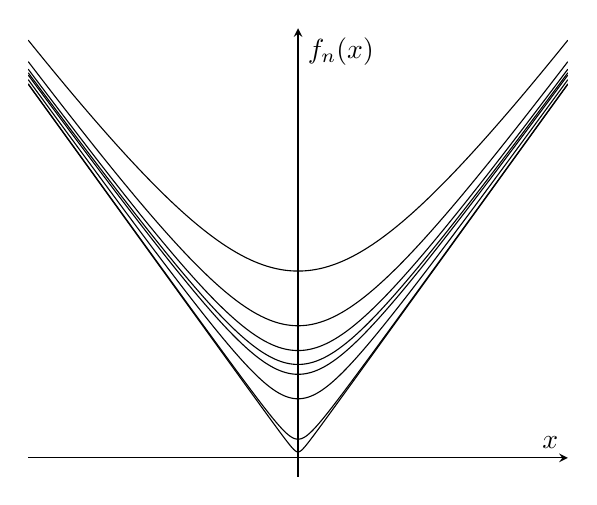
\begin{tikzpicture}
    \begin{axis}[axis x line=middle,axis y line=middle,
		xtick=\empty,ytick=\empty,
		xlabel={$x$},ylabel={$f_n(x)$},
		samples=1000,
		xmin=-2,xmax=2,
		ymin=-0.1,ymax=2.3]
    \addplot[domain=-2:2] {(x^2+1)^0.5};
    \addplot[domain=-2:2] {(x^2+0.5)^0.5};
    \addplot[domain=-2:2] {(x^2+0.33)^0.5};
    \addplot[domain=-2:2] {(x^2+0.25)^0.5};
    \addplot[domain=-2:2] {(x^2+0.2)^0.5};
    \addplot[domain=-2:2] {(x^2+0.1)^0.5};
    \addplot[domain=-2:2] {(x^2+0.01)^0.5};
    \addplot[domain=-2:2] {(x^2+0.001)^0.5};
    \end{axis}
\end{tikzpicture}
\end{center}
\end{example}

\begin{thm}
$(f_n)\subset C^1 [a,b]$. Suppose $f_n \longrightarrow f:[a,b]\rightarrow \mathbb R$ and $f_n' \rightrightarrows g:[a,b]\rightarrow \mathbb R$. Then $f \in C^1 [a,b]$ and $f'=g$.

In other words,
\[
\left(\lim_{n\rightarrow \infty} f_n \right)' = \lim_{n\rightarrow \infty} f_n' .
\]
\end{thm}
\begin{proof}
We have $(f_n') \subset C[a,b]$. Since $g$ is the uniform limit, $g\in C[a,b]$ is integrable. We write
\[
\int_a^x g = \int_a^x \lim_{n\rightarrow \infty} f_n' \underbrace{=}_{\text{Theorem 3.1.15}} \lim_{n\rightarrow \infty} \int_a^x f_n' \underbrace{=}_{\text{FTC}} \lim_{n\rightarrow \infty} \left(f_n(x)-f_n(a)\right) = f(x)-f(a),
\]
i.e. $f(x)=f(a)+\int_a^x g$, so $f'(x)=g(x)$ by FTC. Since $g$ is continuous, $f\in C^1[a,b]$.
\end{proof}

\subsection{Series of functions}
Let $(f_n)$ be a sequence of functions on $\Omega$. Then a series of functions is also a function
\[
x\mapsto \sum_{n=1}^\infty f_k (x),\quad x\in \Omega .
\]
\begin{defn}
Let
\[
S_n := \sum_{k=1}^n f_k\quad :\Omega \rightarrow \mathbb R,\qquad n\geq 1
\]
be the sequence of partial sums. We say that $\displaystyle \sum_{k=1}^\infty f_k$ converges to $S:\Omega \rightarrow \mathbb R$ pointwise (uniformly) if $S_n\rightarrow (\rightrightarrows) S$.
\end{defn}

\begin{thm}
Let $(f_n)$ be a sequence of integrable functions on $[a,b]$ such that $\displaystyle \sum_{k=1}^\infty f_k$ converges uniformly. Then
\[
\sum_{k=1}^\infty f_k\quad :[a,b]\rightarrow \mathbb R
\]
is integrable and
\[
\int_a^b \sum_{k=1}^\infty f_k = \sum_{k=1}^\infty \int_a^b f_k .
\]
i.e. series can be integrated term by term.
\end{thm}
\begin{proof}
Consider
\[
S_n := \sum_{k=1}^n f_k,\qquad S:=\sum_{k=1}^\infty f_k
\]
and we know $S_n \rightrightarrows S$. By linearity $S_n$ is integrable. By Theorem 3.1.15, $S$ is then integrable, and moreover
\[
\int_a^b S = \lim_{n\rightarrow \infty}\int_a^b S_n .
\]
So
\[
\int_a^b \sum_{k=1}^\infty f_k = \lim_{n\rightarrow \infty} \int_a^b \sum_{k=1}^n f_k \underbrace{=}_{\text{linearity}} \lim_{n\rightarrow \infty} \sum_{k=1}^n \int_a^b f_k = \sum_{k=1}^\infty \int_a^b f_k .
\]
\end{proof}

\begin{example}[Do everything by hand]
Let $\lambda >0$ and define
\[
S(x):=\sum_{k=1}^\infty e^{-\lambda kx},\quad x\in [1,\infty) .
\]
What is $\int_1^\infty S$?

Notice that the series converges uniformly on $[1,\infty)$: let
\[
S_n(x):=\sum_{k=1}^n e^{-\lambda k x},
\]
then
\[
|S_n(x)-S_m(x)|=\left|\sum_{k=m+1}^n e^{-\lambda k x}\right| \leq e^{-\lambda m} \left|\sum_{k=0}^\infty e^{-\lambda k \cdot 1} \right| \rightarrow 0
\]
since it's geometric. So it's Cauchy therefore it's uniformly convergent. Therefore we can integrate it term by term:
\[
\begin{aligned}
\int_1^\infty S &= \int_1^\infty \sum_{k=1}^\infty e^{-\lambda k x} \ \mathrm d x = \sum_{k=1}^\infty \int_1^\infty e^{-\lambda k x} \ \mathrm d x \\&= \sum_{k=1}^\infty \frac{1}{\lambda k} e^{-\lambda k} = \frac{1}{\lambda} \sum_{k=1}^\infty \frac{1}{k}\left(e^{-\lambda}\right)^k \\&= \frac{1}{\lambda} \log \left(1-e^{-\lambda} \right).
\end{aligned}
\]
\end{example}
Checking that applying Theorem 3.3.2 here to improper integrals is legitimate is left as an exercise.

\begin{remark}
We can then integrate any function given by uniformly convergent Taylor or Fourier series and set the answer as an infinite sum.
\end{remark}

\begin{thm}
$\displaystyle (f_k) \subset C^1 [a,b] : \sum_{k=1}^\infty f_k$ converges pointwise and $\displaystyle \sum_{k=1}^\infty f_k'$ converge uniformly. Then
\[
x\mapsto \sum_{k=1}^\infty f_k \in C^1[a,b]
\]
and
\[
\left(\sum_{k=1}^\infty f_k\right)' = \sum_{k=1}^\infty f_k' .
\]
i.e. series can be differentiated term by term.
\end{thm}
\begin{proof}
Let
\[
S_n := \sum_{k=1}^n f_k ,\quad S := \sum_{k=1}^\infty f_k
\]
Given that $S_n \rightarrow S$, $S_n' \rightrightarrows g$, we have, by Theorem 3.2.10, $S\in C^1[a,b]$ and $\displaystyle S'=\lim_{n\rightarrow \infty} S_n'$.

We use the fact that $(f_n) \subset C^1[a,b] \Rightarrow S_n= \in C^1[a,b]$ (algebra of differentiable functions).

Therefore
\[
\left(\sum_{k=1}^n f_k \right)' = \lim_{n\rightarrow \infty} \sum_{k=1}^n f_k' = \sum_{k=1}^\infty f_k' .
\]
\end{proof}

\begin{thm}[Weierstrass $M$-test]
Let $(f_k)$ be a sequence of functions on $\Omega \subset \mathbb R$. Suppose $\forall k\in \mathbb N,\ \exists M_k \geq 0 : |f_k|\leq M_k$ where $\sum_{k=1}^\infty M_k < \infty$. Then $\sum_{k=1}^\infty f_k$ converges uniformly on $\Omega$.
\end{thm}
\begin{proof}
\[
\sum_{k=1}^\infty M_k < \infty
\]
if and only if $\displaystyle \left(\sum_{k=1}^n M_k \right)$ is Cauchy if and only if
\[
\forall \varepsilon>0,\ \exists N_\varepsilon : n,m>N_\varepsilon \Rightarrow \left|\sum_{k=1}^n M_k - \sum_{k=1}^m M_k \right|<\varepsilon .
\]
Then $\forall x\in \Omega$,
\[
|S_n(x) - S_m(x)| =\left|\sum_{k=m+1}^n f_k(x)\right| \leq \sum_{k=m+1}^n |f_k(x)| \leq \sum_{k=m+1}^n M_k <\varepsilon .
\]
Therefore $(S_n)$ is Cauchy, therefore uniformly convergent.
\end{proof}

\subsection{3 non-examinable (but exciting!) topics}
\subsubsection{Continuous but nowhere differentiable functions}
Natural example: trajectory of a Brownian particle (sample path of a stochastic process known as Brownian motion)

We will explain construction of the Weierstrass function (1872).

The starting point:
\[
\phi: \mathbb R \rightarrow \mathbb R,\quad x\mapsto \dist (x,\mathbb Z)
\]
Our function will be constructed as a limit of the series of piecewise linear functions built out of $\phi$.
\begin{remark}
Lévy (1950) used this idea for his rigorous construction of Brownian motion.
\end{remark}
\begin{center}
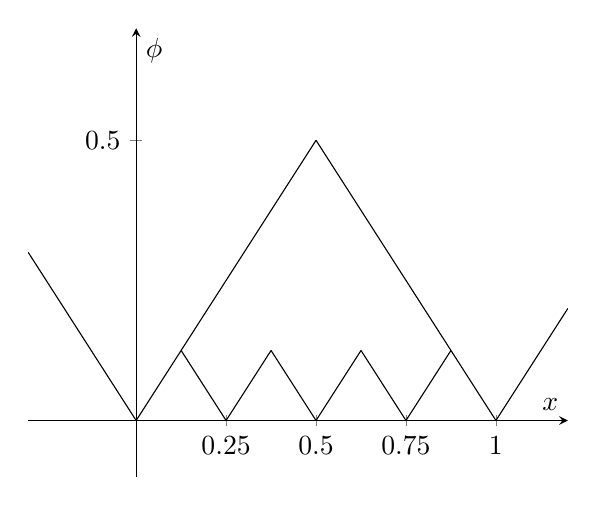
\begin{tikzpicture}
    \begin{axis}[axis x line=middle,axis y line=middle,
		xtick={0.25,0.5,0.75,1},ytick=0.5,
		xlabel={$x$},ylabel={$\phi$},
		samples=1000,
		xmin=-0.3,xmax=1.2,
		ymin=-0.1,ymax=0.7]
    \addplot[domain=-0.3:0] {-x};
    \addplot[domain=0:0.5] {x};
    \addplot[domain=0.5:1] {-x+1};
    \addplot[domain=1:1.2] {x-1};
    
    \addplot[domain=0.125:0.25]{-x+0.25};
    \addplot[domain=0.25:0.375]{x-0.25};
    \addplot[domain=0.375:0.5]{-x+0.5};
    \addplot[domain=0.5:0.625]{x-0.5};
    \addplot[domain=0.625:0.75]{-x+0.75};
    \addplot[domain=0.75:0.875]{x-0.75};
    \end{axis}
\end{tikzpicture}
\end{center}
It's sometimes called the Sawtooth function.

Obvious properties:
\begin{enumerate}
    \item $\phi$ is continuous
    \item $\phi$ is periodic, i.e. $\phi(x+1)=\phi(x) \ \forall x\in \mathbb R$
    \item $\phi$ is piecewise linear
    \item $\phi'(x) \in \{\pm 1\}$ at all $x$ where $\phi'$ is defined
\end{enumerate}
We can write a formula:
\[
\phi(x) = \left\{\begin{aligned}
&x-\lfloor x \rfloor, \qquad &\lfloor x \rfloor \leq x \lfloor x \rfloor+\frac12 \\
&\lfloor x \rfloor +1-x,\qquad &\lfloor x \rfloor+\frac12 <x<\lfloor x \rfloor+1
\end{aligned} \right.
\]
Now define Weierstrass function
\[
f:\mathbb R \rightarrow \mathbb R,\quad x\mapsto \sum_{n=0}^\infty f_n(x),\quad n>0
\]
where $\displaystyle f_n(x) = \frac{1}{4^n} \phi (4^n x)$. So property 4 still holds, $f_0$ is just $\phi$, and $f_1$ is drawn in the same plot above.

\begin{claim}
$f$ is continuous on $\mathbb R$.
\end{claim}
\begin{proof}
We know $\|\phi\|_\infty =\frac12$ and
\[
\|f_n\| = \left\| \frac{1}{4^n} \phi (4^n x) \right\|_\infty = \frac{1}{4^n} \underset{\mathbb R}{\sup} \left| \phi (4^n x) \right| = \frac{1}{4^n} \underset{\mathbb R}{\sup} |\phi| = \frac{1}{4^n}\cdot \frac12 < \frac{1}{4^n}.
\]
Moreover,
\[
\sum_{k=0}^\infty \frac{1}{4^n} < \infty \qquad \text{(geometric)},
\]
therefore $\sum_{k=0}^\infty f_k$ converges uniformly on $\mathbb R$ by his own $M$-test. So
\[
\sum_{k=0}^n f_k \rightrightarrows \sum_{k=0}^\infty f_k = f
\]
and $f$ is continuous by continuity of $f_k$ .
\end{proof}

\begin{claim}
$f$ is nowhere differentiable.
\end{claim}
\begin{proof}
We would like to show that for any $x_0 \in \mathbb R$,
\[
\lim_{h\rightarrow 0} \frac{f(x+h)-f(x)}{h}
\]
doesn't exist. It suffices to show that we can find a sequence $(h_n)_{n\geq 0} \subset \mathbb R$ such that
\begin{enumerate}
    \item $h_n \rightarrow 0$ ,
    \item $\displaystyle \lim_{h_n\rightarrow 0} \frac{f(x+h_n)-f(x)}{h_n}$ doesn't exist .
\end{enumerate}
Define $\displaystyle h_n=\pm \frac{1}{4^{n+1}}$ where the sign is chosen carefully in such a way that
\[
4^n x_0,\ 4^n (x_0+h_n) \in \left[ k,k\pm \frac12 \right]
\]
for some $k\in \mathbb Z$. (These points belong either to $\left[ k- \frac12 ,k \right]$ or $\left[ k,k\pm \frac12 \right]$ for some integer $k$. The above is just shorthand notation. In particular, we are choosing the sign so that the two points are not separated by a point at which the function is not differentiable.)
\begin{center}
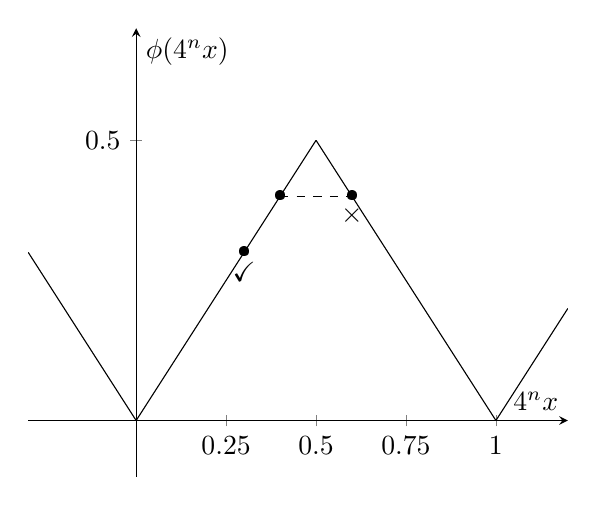
\begin{tikzpicture}
    \begin{axis}[axis x line=middle,axis y line=middle,
		xtick={0.25,0.5,0.75,1},ytick=0.5,
		xlabel={$4^n x$},ylabel={$\phi(4^n x)$},
		samples=1000,
		xmin=-0.3,xmax=1.2,
		ymin=-0.1,ymax=0.7]
    \addplot[domain=-0.3:0] {-x};
    \draw[dashed] (axis direction cs:0.7,0.5) -- (axis direction cs:0.9,0.5);
    \node at (axis direction cs:0.7,0.5) {\textbullet};
    \node at (axis direction cs:0.9,0.5) {\textbullet};
    \node[below] at (axis direction cs:0.9,0.5) {$\times$};
    \node at (axis direction cs:0.6,0.4) {\textbullet};
    \node[below] at (axis direction cs:0.6,0.4) {\checkmark};
    \addplot[domain=0:0.5] {x};
    \addplot[domain=0.5:1] {-x+1};
    \addplot[domain=1:1.2] {x-1};
    \end{axis}
\end{tikzpicture}
\end{center}
Then clearly $\displaystyle \lim_{n\rightarrow \infty} h_n = 0$, and $\displaystyle f_n\left. \right|_{[x_0,x_0+h_n]}$ has a constant slope equal to $\pm 1$. We then write
\begin{equation}
\frac{f_n(x_0+h_n)-f_n(x_0)}{h_n} = \frac{\phi (4^n x_0+4^n h_n)-\phi (4^n x_0)}{4^n h_n} \in \{\pm 1\}.
\end{equation}
Now fix $m \geq n+1$, and we have
\begin{equation}
\frac{f_m(x_0+h_n)-f_m(x_0)}{h_n} = \frac{\phi (4^m x_0+\overbrace{4^m h_n}^{\in \mathbb Z})-\phi (4^m x_0)}{4^m h_n} =0
\end{equation}
since $\phi$ is periodic with period 1. And for $m<n$,
if $f_m$ is not smooth at points $x$, i.e.
\[
4^m x = \frac{k}{2} \quad \text{for }k\in \mathbb Z,
\]
then for the same $x$,
\[
4^n x = 4^{n-m} (4^m x) = 4^{n-m} \left( \frac{k}{2} \right) = \frac{k'}{2}
\]
where $k'=4^{n-m}\cdot k,\ n\geq m$. This means if $m$ is not smooth then $n$ is not either.

We conclude that the set of points at which $f_m$ changes slope is a subset of points where $f_n$ changes slope, $n\geq m$. Also, if $f_n\left. \right|_{[x_0,x_0+h_n]}$ has constant slope then so does $f_m\left. \right|_{[x_0,x_0+h_n]}, \ n\geq m$.

In plain English, the indifferentiable points of $f_n$ are also indifferentiable points of $f_{n+1}$. Finally, we write
\[
\begin{aligned}
\frac{f(x+h_n)-f(x_n)}{h_n} &= \lim_{N\rightarrow \infty} \sum_{m=0}^N \frac{f_m (x_0+h_n)-f_m(x_0)}{h_n} \\&= \sum_{m=0}^n \frac{f_m (x_0+h_n)-f_m(x_0)}{h_n} \qquad \text{by (4)} \\&= \sum_{m=0}^n \varepsilon_m \qquad \text{by (3)}
\end{aligned}
\]
where $\varepsilon_m\in \{\pm 1\}$. Taking the limits to get to derivative, we have
\[
\lim_{n\rightarrow \infty} \frac{f(x+h_n)-f(x_n)}{h_n} = \sum_{m=0}^\infty \varepsilon_m
\]
which diverges! Hence desired result.
\end{proof}

\subsubsection{Space-filling curves}
\underline{Aim}: construct a surjective, continuous map from $[0,1]$ to $[0,1]\times [0,1]$. \\

Surjective is not that hard: define $\gamma_0:[0,1]\rightarrow [0,1]^2$ like this: write numbers in $[0,1]$ as $0.a_1 a_2 a_3\ldots$ where $a_i\in \{0,1,\ldots,9\}$. Then take the two subsequences and form a ordered pair, an odd and an even: $(0.a_1a_3a_5\ldots, 0.a_2a_4a_6\ldots )$. It's in fact bijective.

But it's not continuous! So is it possible to reach the aim? The answer is of course positive.

We will review Hilbert's construction of the curve (1891), the very first example is due to Peano (1890), as a uniformly convergent sequence of piecewise linear curves.

Terminology:
\begin{itemize}
    \item A \textit{curve} in $\mathbb R^2$ is a continous map $\beta:[0,1]\rightarrow \mathbb R^2$, $t\mapsto \beta(t)=(\beta_1(t),\beta_2(t))$
    \item It's useful recalling that $\beta$ is \textit{continuous} at $t_0\in [0,1]$ if
    \[
    \forall \varepsilon >0, \ \exists \delta_\varepsilon>0: |t-t_0|<\delta_\varepsilon \Rightarrow |\beta(t)-\beta(t_0)|<\varepsilon ,
    \]
    and this if and only if $\beta_1,\beta_2:\mathbb R\rightarrow \mathbb R$ are continuous
    \item The \textit{image} of $\beta$, $\text{Im} (\beta)=\beta([0,1])\subset \mathbb R^2$
    \item A curve $\gamma:[0,1]\rightarrow[0,1]^2$ is called \textit{space-filling} or SPC if $\text{Im}(\gamma)=[0,1]^2$.
\end{itemize}
We now define the Hilbert curve
\[
\gamma := \lim_{n\rightarrow \infty} \gamma_n
\]
where $\gamma_n \rightrightarrows \gamma$. And here's the construction. Denote unit square as $S_0$.

\begin{enumerate}
    \item Divide into four, connect centres of squares counterclockwise, and connect the two top centres with two vertices. Before parameterising $\gamma_1$, we label the smaller squares as $S_{0.0},S_{0.1},S_{0.2},S_{0.3}$ counterclockwise. Now notice $S_{0,n} \subset S_0$. We want our parametrisation satisfies that $\gamma_1 \left( \left[0,\frac14 \right]\right) \subset S_{0,0},\ \gamma_1 \left( \left[\frac14,\frac12 \right]\right) \subset S_{0,1},\ \gamma_1 \left( \left[\frac12,\frac34 \right]\right) \subset S_{0,2},\ \gamma_1 \left( \left[\frac34,1 \right]\right) \subset S_{0,3}$. We can then write:
    \[
    \gamma_1(t) = \left\{\begin{aligned}
        &\left(2t,1-2t\right),\qquad & 0\leq t < \frac18 \\
        &\left(\frac14,1-2t\right),\qquad & \frac18 \leq t < \frac38 \\
        &\left(2t-\frac12,\frac14\right),\qquad & \frac38 \leq t < \frac58 \\
        &\left(\frac34, 2t-1\right),\qquad & \frac58 \leq t <\frac78 \\
        &\left(2t-1, 2t-1\right),\qquad & \frac78 \leq t \leq 1
    \end{aligned} \right .
    \]
    \begin{figure}[h]
    \centering
    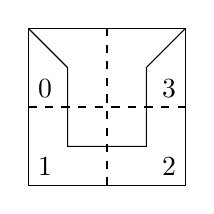
\begin{tikzpicture}[scale=2]
    \draw (0,0)node[anchor=south west]{1} -- (1,0)node[anchor=south east]{2} -- (1,1) -- (0,1) -- (0,0);
    \draw[dashed] (0,0.5)node[anchor=south west]{0} -- (1,0.5)node[anchor=south east]{3};
    \draw[dashed] (0.5,0) -- (0.5,1);
    \draw (0,1) -- (0.25,0.75) -- (0.25,0.25) -- (0.75,0.25) -- (0.75,0.75) -- (1,1);
\end{tikzpicture}
    \caption*{$\gamma_1$}
    \label{fig:gamma1}
\end{figure}
\item Now create 4 copies of $\text{Im}(\gamma_1)$ and connect them together in 4 divided squares to create $\gamma_2$:

\begin{figure}[h]
    \centering
    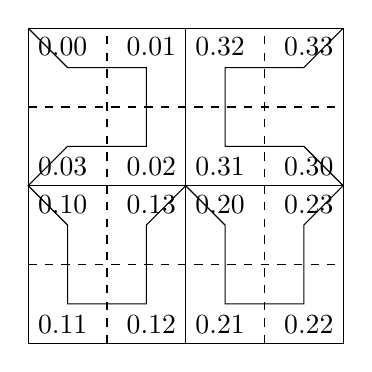
\begin{tikzpicture}[scale=4]
    \draw (0,0)node[anchor=south west]{0.11} -- (1,0)node[anchor=south east]{0.22} -- (1,1)node[anchor=north east]{0.33} -- (0,1)node[anchor=north west]{0.00} -- (0,0);
    \draw (0,0.5)node[anchor=south west]{0.03} node[anchor=north west]{0.10} -- (1,0.5)node[anchor=north east]{0.23} node[anchor=south east]{0.30};
    \draw (0.5,0)node[anchor=south east]{0.12} node[anchor=south west]{0.21} -- (0.5,1)node[anchor=north east]{0.01} node[anchor=north west]{0.32};
    \draw[dashed] (0,0.25) -- (1,0.25);
    \draw[dashed] (0,0.75) -- (1,0.75);
    \draw[dashed] (0.25,0) -- (0.25,1);
    \draw[dashed] (0.75,0) -- (0.75,1);
    \draw (0,1) -- (0.125,0.875) -- (0.375,0.875) -- (0.375,0.625) -- (0.125,0.625) -- (0,0.5) -- (0.125, 0.375) -- (0.125,0.125) -- (0.375,0.125) -- (0.375,0.375) -- (0.5,0.5)node[anchor=south east]{0.02} node[anchor=north east]{0.13} node[anchor=north west]{0.20} node[anchor=south west]{0.31} -- (0.625,0.375) -- (0.625,0.125) -- (0.875,0.125) -- (0.875,0.375) -- (1,0.5) -- (0.875,0.625) -- (0.625,0.625) -- (0.625,0.875) -- (0.875,0.875) -- (1,1);
\end{tikzpicture}
    \caption*{$\gamma_2$}
    \label{fig:gamma2}
\end{figure}
The lower two are just translations, but we have to rotate for the upper two ($\frac{\pi}{2}$ counterclockwise and clockwise respectively) to keep the curve starting from top left and end at top right. To make sure the direction of parameterisation makes sense, we also have to reflect horizontally. And finally we need to scale it down by a factor of 2 to make it a unit square.

We again, as before, enumerate the 4 squares of size $\frac12 \times \frac12$ as $S_{0.m},\ 0\leq m\leq 3$. We also have 16 squares of size $\frac14\times \frac14$, and we enumerate them as $S_{0.m_1m_2},\ 0\leq m_1,m_2\leq 3$, where $m_1$ is the index of the $\frac12 \times \frac12$ squares and $m_2$ is similar to $m$ as in how we enumerate $S_{0.m}$'s. Note
\[
S_{0,m_1,m_2}\subset S_{0,m_1} \ \forall m_1,m_2 .
\]
For parametrisation of $\gamma_2$, we notice 
\[
\gamma_2(t) =\left\{\begin{aligned}
&A_0 \gamma_1 (4t), &\qquad 0\leq t\leq \frac14 \\
&A_1 \gamma_1 (4t-1), &\qquad \frac14\leq t\leq \frac12 \\
&A_2 \gamma_1 (4t-2), &\qquad \frac12\leq t\leq \frac34 \\
&A_3 \gamma_1 (4t-3), &\qquad \frac34\leq t\leq 1 
\end{aligned}\right. ,
\]
(basically speed it up in the smaller squares and impose lags to make sure every part of it satisfy the original parametrisation with $t$ ranging from 0 to 1). So we don't need to invent a new parametrisation. Notice $\gamma_2$ goes through all 16 squares and spend $\frac{1}{16}$ of the time in each of it. Let us treat $0.m_1m_2$ now as quarternary fractions:
\[
0.m_1m_2 = m_1 \times 4^{-1}+m_2\times 4^{-2}= \frac{m_1}{4}+\frac{m_2}{16},
\]
since we keep dividing by 4, it's better to use base 4 than base 10. Notice by construction
\[
\gamma_2 \left( \left[m_1m_2,m_1m_2+1\right] \frac{1}{4^2}\right) \subset S_{0.m_1m_2}
\]
where $m_1m_2$, a quaternary number, is equal to $m_1\times 4^1+m_2\times 4^0=4m_1+m_2$.
\item Now we can construct $\gamma_{n+1}$ from $\gamma_n$ generally, in a way exactly the same as how $\gamma_2$ is constructed from $\gamma_1$: enumerate counterclockwise, translate, rotate, reflect and scale. And we have a new index for smallest squares, namely $S_{0.m_1m_2\ldots m_n}$. Note $S_{0.m_1\ldots m_n} \subset S_{0.m_1\ldots m_k}$ for any $k\leq n$. Parametrisation of $\gamma_{n+1}$ is again recursive like what we wrote for $\gamma_2$.
\end{enumerate}

Now we have $\gamma_n: [0,1] \rightarrow [0,1]^2$ such that \begin{itemize}
    \item it's piecewise linear, continuous, passing through centre of each $4^n$ squares of size $\frac{1}{2^n}$
    \item $\gamma_n \left(\left[ 0.m_1\ldots m_n, 0.m_1\ldots m_n + \frac{1}{4^n} \right] \right) \subset S_{0.m_1\ldots m_n}$ .
\end{itemize}
We need to establish \begin{itemize}
    \item The limit $\displaystyle \lim_{n\rightarrow \infty} \gamma_n$ exists and is continuous
    \item $\gamma$ is space-filling.
\end{itemize}
Let's do this part by part.
\begin{enumerate}
    \item We know $\gamma_n$ are continuous, so to prove $\gamma$ is continuous we only need to construct uniform continuity, but we don't know the limit, so instead we construct uniform Cauchy which is equivalent.
    
    Fix $t\in [0,1]$. For any $n\in \mathbb N,$
    \[
    \begin{aligned}
    \exists m_1,\ldots,m_n \in \{0,1,2,3\} : t&\in \left[0.m_1\ldots m_{n+1},0.m_1\ldots m_{n+1} + \frac{1}{4^{n+1}} \right] \\&\subset \left[0.m_1\ldots m_{n},0.m_1\ldots m_{n} + \frac{1}{4^{n}} \right] .
    \end{aligned}
    \]
    Since clearly
    \[
    0.m_1\ldots m_{n+1}\geq 0.m_1\ldots m_n
    \]
    and
    \[
    0.m_1\ldots m_{n+1} + \frac{1}{4^{n+1}}\leq 0.m_1\ldots m_n + \frac{1}{4^{n+1}} +\frac{3}{4^{n+1}} = 0.m_1\ldots m_n + \frac{1}{4^n}.
    \]
    This means $\gamma_n(t),\gamma_{n+1}(t) \in S_{0.m_1\ldots m_n}$. So $|\gamma_{n+1}(t)-\gamma_n(t)|\leq \frac{\sqrt 2}{2^n}$, length of diagonal. So $\forall m,n \in \mathbb N,\ \forall t\in [0,1]$, we have
    \[
    \begin{aligned}
    |\gamma_{n+m}(t)-\gamma_n(t)| &\leq |\gamma_{n+m}(t)-\gamma_{n+m-1}(t)|+|\gamma_{n+m-1}(t)-\gamma_{n+m-2}(t)|+\\& \cdots+|\gamma_{n+1}(t)-\gamma_n (t)| \\&\leq \sqrt 2 \left(2^{-n-m+1}+2^{-n-m}+\cdots + 2^{-n+1}\right) \\& \leq \sqrt 2 \cdot 2^{-n+1} \underbrace{\sum_{k=0}^\infty 2^{-k}}_{\text{geometric}=2} \rightarrow 0.
    \end{aligned}
    \]
    as desired.
    \item We now want $\forall p\in [0,1]^2,\ \exists t_0 \in [0,1]:\gamma(t_0)=p$. By construction, $\forall d>0,\ \exists t\in [0,1] : |\gamma(t)-p|<d$: how? Consider partition of $[0,1]^2$ by $4^n$ squares of size $\frac{1}{2^n}$. Then $\forall \tau_n \in \left[0.m_1\ldots m_n, 0.m_1\ldots m_n+\frac{1}{4^n} \right]$, $\gamma_n(\tau_n)\in S_{0.m_1\ldots m_n}$. Choose $0.m_1\ldots m_n$ such that $S\in S_{0.m_1\ldots m_n}$. Then $|\gamma_n (\tau_n)-p|<\frac{\sqrt 2}{2^n}$. So
    \[
    |\gamma(\tau_n)-p| \leq |\gamma(\tau_n)-\gamma_n(\tau_n)|+|\gamma_n(\tau_n)-p| \leq \|\gamma-\gamma_n\|_\infty + \frac{\sqrt 2}{2^n} \rightarrow 0.
    \]
    Now set $d=\frac1n,\ n\in \mathbb N$. Then we are dealing with a sequence of time $(t_n):\lim_{n\rightarrow \infty} |\underbrace{\gamma(t_n)-p}_{\leq \frac1n}|=0.$ Equivalently, $\displaystyle \lim_{n\rightarrow \infty} \gamma(t_n)=p$. But $(t_n)_{n\geq 1}$ doesn't have to converge. But! $(t_n) \subset [0,1]$ which is bounded closed. So apply Bolzano–Weierstrass to get a subsequence $t_{n_k}$. Then $\displaystyle \lim_{k\rightarrow \infty} t_{n_k}=t_0 \in [0,1]$. So
    \[
    p=\lim_{k\rightarrow \infty} \gamma\left(t_{n_k}\right) \underbrace{=}_{\text{continuity}}\gamma\left(\lim_{k\rightarrow \infty} t_{n_k}\right)=\gamma(t_0) .
    \]
\end{enumerate}
Finally we ask: is $\gamma$ bijective? It's actually not injective, since there is a dense set of points of self intersection: $\gamma(t_1)=\gamma(t_2)$ but $t_1 \neq t_2$.
\begin{thm}[Netto's]
A bijection between two manifolds of different dimensions (hypercubes in $\mathbb R^n$) cannot be continuous.
\end{thm}

\subsubsection{Cantor function, aka Devil's staircase}
Let $(f_n)_{n\geq 0}$ be a sequence of functions on $[0,1]$. $f_0(x):=x$. Then
\[
f_{n+1}(x) := \left\{\begin{aligned}&\frac12 f_n (3x) \qquad &0\leq x \leq \frac13 \\ &\frac12 \qquad &\frac13 <x < \frac23 \\ &\frac12 + \frac12 f_n(3x-2) \qquad &\frac23 \leq x \leq 1\end{aligned} \right.
\]

\begin{center}
\begin{tikzpicture}
    \begin{axis}[axis x line=middle,axis y line=middle,
        xtick={1/3,2/3,1},xticklabels={$\frac13$,$\frac23$,$1$},
        ytick={1/4,1/2,3/4,1},,yticklabels={$\frac14$,$\frac12$,$\frac34$,$1$},
		xlabel={$y$},ylabel={$x$},
		samples=1000,
		xmin=-0.1,xmax=1.1,
		ymin=-0.1,ymax=1.1,
		legend pos=outer north east]
    \addplot[domain=0:1,blue] {x};
    
    \addplot[domain=0:1/3,red] {3*x/2};
    \addplot[domain=1/3:2/3,red]{1/2};
    \addplot[domain=2/3:1,red]{1/2+(3*x-2)/2};
    
    \addplot[domain=0:1/9]{9*x/4};
    \addplot[domain=1/9:2/9]{1/4};
    \addplot[domain=2/9:1/3]{9*(x-2/9)/4+1/4};
    \addplot[domain=2/3:7/9]{9*(x-2/3)/4+1/2};
    \addplot[domain=7/9:8/9]{1/4+1/2};
    \addplot[domain=8/9:1]{9*(x-2/9-2/3)/4+1/4+1/2};
    
    \legend{$f_0$,$f_1$,,,$f_2$}
    \end{axis}
\end{tikzpicture}
\end{center}

\underline{Observations}:
\begin{itemize}
    \item $f_n:[0,1]\rightarrow [0,1]$
    \item increasing
    \item $f_{n+1}(0) = \frac12 f_n(0) = \frac12 ^2 f_{n-1}(0) = \cdots = \frac12 ^{n+1} f_0(0)=0$
    \item $f_{n+1}(1) = \frac12 + \frac12 f_n(1) \underbrace{=}_{\text{induction}} = \frac12 + \frac12=1 $
\end{itemize}
\underline{Claims}:
\begin{enumerate}
    \item $f_n \in C[0,1] \ \forall n\geq 0$.
    \begin{proof}
    Use induction. Obviously $f_0 \in C[0,1]$. Now suppose $f_n$ is continuous. Then $f_{n+1}$ is continuous on $\left[0,\frac13\right)\cup \left(\frac13,\frac23\right)\cup \left(\frac23,1\right]$ by construction. We then only need to check two points $x=\frac13,\frac23.$
    
    We have
    \[
    \lim_{x\uparrow \frac13} f_{n+1}(x) = \lim_{x\uparrow \frac13} \frac12 f_n (3x) = \frac12 \lim_{x\uparrow 1} f_n(x) = \frac12 f_n(1) = \frac12,
    \]
    and similarly $\lim_{x\downarrow \frac13} f_{n+1}(x) = \frac12$. Two limits agree so continuous at $\frac13$. Similarly it's continuous at $\frac23$.
    \end{proof}
    \item The sequence $(f_n) \in C[0,1]$ is uniformly Cauchy. Therefore the limit $f:=\lim_{n\rightarrow \infty} f_n$ is continuous on $[0,1]$, which is defined as Cantor function.
    \begin{proof}
    We have
    \[
    \begin{aligned}
    \|f_{n+1}-f_n\|_\infty &\leq \max \left\{ \underset{\left[0,\frac13\right]}{\sup} |f_{n+1}(x)-f_n(x)|,\underbrace{\underset{\left[\frac13,\frac23\right]}{\sup} |f_{n+1}(x)-f_n(x)|}_{0},\underset{\left[\frac23,1\right]}{\sup} |f_{n+1}(x)-f_n(x)|  \right\} \\
    &=\max \left\{\frac12 \underset{\left[0,\frac13\right]}{\sup} \left|f_n(3x)-f_{n-1}(3x) \right|,\frac12 \underset{\left[\frac23,1\right]}{\sup} \left|f_n(3x)-f_{n-1}(3x) \right| \right\} \\
    &= \max \left\{ \frac12 \underset{[0,1]}{\sup} |f_n(x) - f_{n-1} (x)|,\frac12 \underset{[0,1]}{\sup} |f_n(x) - f_{n-1} (x)| \right\} \\
    &= \frac12 \underset{[0,1]}{\sup} |f_n(x) - f_{n-1} (x)| \\
    &= \frac12 \underbrace{\|f_n-f_{n-1}\|_\infty}_{\leq C} .
    \end{aligned}
    \]
    If we iterate this we have
    \[
    \|f_{n+1}-f_n\|_\infty \leq \frac12 \|f_n-f_{n-1}\|_\infty \leq \frac12 ^2 \|f_{n-1}-f_{n-2}\|_\infty \leq \cdots \leq \frac12 ^n \|f_1-f_0\|_\infty .
    \]
    So $\forall n,m \in \mathbb N,$
    \[
    \begin{aligned}
    \|f_{n+m}-f_n\|_\infty &\leq \|f_{n+m}-f_{n+m-1}\|_\infty + \|f_{n+m-1}-f_{n+m-2}\|+\cdots + \|f_{n+1}-f_n\|_\infty \\&\leq C \left(\frac12^{n+m} + \frac12 ^{n+m-1} + \cdots + \frac12 ^{n+1} \right) \\&\leq \frac12 ^{n+1} C \underbrace{\sum_{k=1}^\infty \frac12 ^k}_{\text{geometric}} \rightarrow 0.
    \end{aligned}
    \]
    \end{proof}
\end{enumerate}

\underline{Properties of Cantor function}:
\begin{enumerate}
    \item $f:[0,1]\rightarrow [0,1]$ is continuous, monotonically increasing and $f(0)=0,\ f(1)=1$. By IVT $f$ is surjective. Also by Theorem 1.1.15 it's integrable.
    \item Take $\lim_{n\rightarrow \infty} f_n$ we have
    \[
    f(x) := \left\{\begin{aligned}&\frac12 f (3x) \qquad &0\leq x \leq \frac13 \\ &\frac12 \qquad &\frac13 <x < \frac23 \\ &\frac12 + \frac12 f(3x-2) \qquad &\frac23 \leq x \leq 1\end{aligned} \right. ,
    \]
    a functional equation for $f$. Therefore
    \[
    \int_0^\frac13 f(x) \ \mathrm d x = \frac12 \int_0^\frac13 f(3x) \ \mathrm d x = \frac16 \int_0^1 f(x) \ \mathrm d x
    \]
    and
    \[
    \int_\frac23^1 f(x) \ \mathrm d x = \frac16 + \frac12 \int_\frac23^1 f(3x-2) \ \mathrm d x = \frac16 +\frac16 \int_0^1 f(x) \ \mathrm d x
    \]
    so
    \[
    \frac16 \int_0^1 f + \frac12 \times \frac13+\frac16+\frac16\int_0^1 f=\int_0^1 f,
    \]
    hence $\int_0^1 f = \frac12$.
    \item We know $f$ is constant on $E_0=\left(\frac13,\frac23 \right).$ Obviously it's also constant on $E_{1,1}=\frac13 E_0,\ E_{1,2}=\frac23+\frac13 E_0$, and $\left.f\right|_{E_{1,1}}=\frac14,\ \left.f\right|_{E_{1,2}}=\frac34$. Moreover they do not overlap since $f$ is continuous. Note $|E_0|=\frac13,\ |E_{1,1}|=|E_{1,2}|=\frac19$.
    
    More generally, if $\left.f\right|_E$ is constant, then it's also constant on $\frac13 E,\ \frac23+\frac13 E$. We iterate this and after $k$ steps we have 
    \[
    E_0,E_{1,1},E_{1,2},E_{2,1},E_{2,2},E_{2,3},E_{2,4},\ldots,E_{k,1},\ldots,E_{k,2^k},
    \]
    a total of $2^{k+1}-1$ intervals of length $\frac13,\frac{1}{3^2},\ldots,\frac{1}{3^{k+1}}$, on which the value of $f$ are
    \[
    \frac{m}{2^{k+1}},\ 1\leq m\leq 2^{k+1}-1,
    \]
    i.e. distinct. Therefore they are disjoint. The miracle here is that the total length of these intervals is
    \[
    \frac13+2\frac{1}{3^2}+4\frac{1}{3^3}+\cdots =\sum_{k=0}^\infty \frac13\cdot \frac{2}{3}^k =\frac{\frac13}{1-\frac23} =1.
    \]
\end{enumerate}
The set $C:=[0,1]\backslash E$ is called Cantor set. Its total length is zero, yet $f:C\rightarrow [0,1]$ is a surjectivity: a standard example in measure theory, fractal geometry, analysis, ...

\begin{remark}
Please take a look at the exercises at the end of week 6 notes, giving a more analytic characteristic of Cantor set and a formula for Cantor function.
\end{remark}

\section{Complex analysis}
\subsection{Review of complex numbers}
$\mathbb C = \{x+iy,\ x,y\in \mathbb R\}$ where $i^2=1$. This gives a field of complex numbers, in other words you can multiply and divide (nonzero denominators).

\begin{center}
\begin{tikzpicture}
    \begin{axis}[axis x line=middle,axis y line=middle,
        xtick={1/2},xticklabels={$x$},
        ytick={1/2,-1/2},yticklabels={$y$,$-y$},
		xlabel={$\Re z$},ylabel={$\Im z$},
		samples=1000,
		xmin=-0.1,xmax=0.7,
		ymin=-0.7,ymax=0.7,
		legend pos=outer north east]
    \addplot[domain=0:0.5] {x};
    \addplot[domain=0:0.5] {-x};
    \end{axis}
\end{tikzpicture}
\end{center}

\begin{notation}[Conjugate]
$\overline{z}:=x-iy$
\end{notation}
\begin{notation}[Modulus]
$|z|:=\sqrt{x^2+y^2}$
\end{notation}

Recall these properties:
\begin{enumerate}
    \item $\overline{\overline{z}}=z$
    \item $\overline{z+w}=\overline{z}+\overline{w}$
    \item $\overline{zw}=\overline{z}\overline{w}$
    \item $z\overline{z}=|z|^2$ and $|z|=|\overline{z}|$
\end{enumerate}

Note there is an isomorphism between $\mathbb R^2 \cong \mathbb C$:$\begin{pmatrix}x\\y\end{pmatrix}=\begin{pmatrix}\Re z \\ \Im z \end{pmatrix}$. This is norm preserving: $|z| = \left\| \begin{pmatrix}x\\y\end{pmatrix} \right\|_{\mathbb R^2}$ (Euclidean norm).
\subsection{Introduction}
\begin{defn}
$(z_n)_{n\in \mathbb N} \subset \mathbb C$ \textit{converges} to $z_0 \in \mathbb C$ if
\[
\forall \varepsilon >0, \ \exists N_\varepsilon : n>N_\varepsilon \Rightarrow |z_n-z_0|<\varepsilon .
\]
Equivalently, $\displaystyle \lim_{n\rightarrow 0} |z_n-z_0|=0$.
\end{defn}

\begin{defn}
$\Omega \subset \mathbb C$ is \textit{open} if
\[
\forall z\in \Omega,\ \exists r>0: \mathbb B_r(z) = \{w\in \mathbb C:|w-z|<r\} \subset \Omega .
\]
where $\mathbb B$ is called an \textit{open ball} (which is open).
\end{defn}
\begin{defn}
$\Omega \subset \mathbb C$ is \textit{closed} if $\Omega^C := \mathbb C \backslash \Omega$ is open.
\end{defn}
\begin{notation}[Closed ball]
$\overline{\mathbb B}_r(z) = \{w\in \mathbb C:|w-z|\leq r\}$
\end{notation}
\begin{defn}
$K\subset C$ is sequentially compact if for any $(z_k)_{k\in \mathbb N} \subset K$ there is a subsequence converging in $K$. (Sequentially compact $\Leftrightarrow$ closed and bounded)
\end{defn}

\begin{defn}
A $\mathbb C$-valued function on $\mathbb C$ is a map $f:\mathbb C \rightarrow \mathbb C$ which can be written as $z=x+iy \mapsto f(z)=u(x,y) + iv(x,y)$.

So $f$ can be thought as a function $\mathbb R^2 \rightarrow \mathbb R^2,\ \begin{pmatrix}x\\y\end{pmatrix} \mapsto \begin{pmatrix} u(x,y) \\ v(x,y) \end{pmatrix}$.
\end{defn}

\begin{defn}
$f:\Omega \subset \mathbb C \rightarrow \mathbb C$ is continuous at $z_0 \in \Omega$ if
\[
\forall \varepsilon >0, \ \exists \delta >0 : \left( z\in \Omega, |z-z_0|<\delta \right) \Rightarrow |f(z)-f(z_0)| < \varepsilon .
\]
Equivalently, $\displaystyle \lim_{z\rightarrow z_0} f(z) = f(z_0)$.
\end{defn}

\begin{defn}
$f:\underbrace{\Omega}_{\text{unless state otherwise this is open}} \rightarrow \mathbb C$ is \textit{complex differentiable} at $z\in \Omega$ if
\[
\lim_{h\rightarrow 0} \frac{f(z+h)-f(z)}{h}
\]
where $h\in \mathbb C$ exists. In this case the limit is called the \textit{(complex) derivative}, denoted $f'(z)$.
\end{defn}

Recall in context of multivariable real functions, $f:\mathbb R^n \rightarrow \mathbb R^k$ is differentiable at $p\in \mathbb R^n$ if $\exists Df(p) \in \mathcal L(\mathbb R^n,\mathbb R^k) :$
\[
\lim_{h\rightarrow 0} \frac{\|f(p+h)-f(p)-Df(p)h\|_k}{\|h\|_n} =0
\]
We cannot divide by $h$ as $\mathbb R^n$ is not a field, but $\mathbb C$ is a field, so formula in Definition 1.1.13 is well-defined, albeit it looks more like a definition of $\frac{\partial f}{\partial x}$. Hence it must exist along \underline{any} curve passing through zero. This means we can derive the simplest necessary condition for existence of complex derivative:
\[
\lim_{\Delta x\rightarrow 0} \lim_{\Delta y\rightarrow 0} \frac{f(z+h)-f(z)}{h}=\lim_{\Delta y\rightarrow 0} \lim_{\Delta x\rightarrow 0} \frac{f(z+h)-f(z)}{h}
\]
where $h=\Delta x+i\Delta y$.

Let $f(z)=u(x,y)+iv(x,y).$ Then
\[
\begin{aligned}
& \lim_{\Delta x\rightarrow 0} \frac{f(z+\Delta x) -f(z)}{\Delta x} = \lim_{\Delta y \rightarrow 0} \frac{f(z+i\Delta y)-f(z)}{i\Delta y} \\
&\quad \ \lim_{\Delta x\rightarrow 0} \frac{(u(x+\Delta x, y) - u(x,y) + i(v(x+\Delta x,y)-v(x,y))}{\Delta x}  \\ &= \lim_{\Delta y\rightarrow 0} \frac{u(x,y+\Delta y)-u(x,y) + i (v(x,y+\Delta y) - v(x,y))}{i\Delta y} 
\end{aligned}
\]
so if we denote partial derivative of $u:\mathbb R^2 \rightarrow \mathbb R$ with respect to $x$, we can write
\[
\frac{\partial u}{\partial x} (x,y) + i \frac{\partial v}{\partial x} (x,y) = \frac{1}{i} \left( \frac{\partial u}{\partial y} (x,y) + i \frac{\partial v}{\partial y}(x,y) \right),
\]
i.e.
\[
\left\{\begin{aligned}
\frac{\partial u}{\partial x}(x,y) &= \frac{\partial v}{\partial y} (x,y) \\
\frac{\partial v}{\partial x}(x,y) &= -\frac{\partial u}{\partial y} (x,y)
\end{aligned} \right.
\]
This is called Cauchy–Riemann equations.

\begin{example}
\begin{enumerate}
    \item $f(z)=z,\ z\in \mathbb C$, the identity map. Then $\forall z\in \mathbb C$,
    \[
    \lim_{h\rightarrow 0} \frac{f(z+h)-f(z)}{h} = \lim_{h\rightarrow 0} \frac{z+h-z}{h} = 1.
    \]
    So $f'(z)=1$.
    \item $g(z) = \overline{z},\ z\in \mathbb C$, conjugation of identity map. Then
    \[
    \lim_{h\rightarrow 0}\frac{g(z+h)-g(z)}{h} = \lim_{h\rightarrow 0} \frac{\overline{h}}{h}
    \]
    which we claim does not exist. Take $h=\rho e^{i\phi}$, then $\frac{\overline{h}}{h} = e^{-2i\phi}$ depends on angle of approach.
    
    It's also reasonable to check if Cauchy–Riemann can verify of this non-differentibility. We write $g=u+iv$ where $u(x,y)=x$ and $v(x,y)=-y$. Then $u_x=1\neq v_y=-1$.
\begin{remark}
However, as a function on $\mathbb R^2 \rightarrow \mathbb R^2$, $\begin{pmatrix}x\\y\end{pmatrix}\mapsto \begin{pmatrix}x\\-y\end{pmatrix}$ is differentiable by existence and continuity of its partial derivatives.
\end{remark}
\end{enumerate}
\end{example}
\begin{remark}
\begin{itemize}[Demystification]
    \item If $\displaystyle f'(z):=\lim_{h\rightarrow 0} \frac{f(x+h)-f(x)}{h}$ exists then clearly $f$ is continuous at $z$.
    \item Let $h(\Delta x):=\begin{pmatrix} \Delta x \\ 0 \end{pmatrix}$ where $\Delta x \rightarrow 0$. Notice that
    \[
    f'(z)=\lim_{\Delta x \rightarrow 0} \frac{f(z+h\Delta x)-f(z)}{h\Delta x}
    \]
    is just the partial derivative $u_x(x,y)+i v_x(x,y)$ which by linearity is just $\displaystyle \frac{\partial}{\partial x} f(z)$. By similar argument we conclude that if $f'(z)$ exists then it equals both partial derivatives $\displaystyle \frac{\partial}{\partial x} f(z)$ and $\displaystyle \frac{1}{i} \frac{\partial}{\partial y} f(z)$.
    \item $(z^n)'=nz^{n-1}$
\end{itemize}
\end{remark}
\begin{defn}
$f:\Omega \subset \mathbb C \rightarrow \mathbb C$ is \textit{analytic} or \textit{holomorphic} at $z\in \Omega$ if $\exists U \in \Omega$, an open neighbourhood of $z$ where $f$ is complex differentiable at its every point.

$f$ is analytic in $\Omega \subset \mathbb C$ if it is differentiable at every point of $\Omega$.
\end{defn}
\begin{defn}
$f:\mathbb C \rightarrow \mathbb C$ is \textit{entire} if it is analytic at every $z\in \mathbb C$.
\end{defn}
\begin{remark}
We can think of $U$ as $\mathbb B_r(z)$ for some $r>0$.
\end{remark}
Why do we need these definitions?
\begin{example}[Functions complex differentiable at one point but not analytic]
Consider $f:z\mapsto |z|^2$. It's differentiable at 0 since
\[
\lim_{h\rightarrow 0} \frac{h\cdot h}{h} = 0.
\]
But if we write $f=u+iv$ then $u=x^2+y^2,\ v=0$. So $u_x=2x,\ v_y=0,\ u_y=2y,\ v_x=0$, i.e. Cauchy–Riemann is only satisfied when $x=y=0$. Therefore $f$ is not analytic at $z=0$.
\end{example}
We have the knowledge of previous Remark. But actually Cauchy–Riemann gives us something more.
\subsection{Algebraic meaning of Cauchy–Riemann}
Consider $z,\overline{z}:\mathbb R^2 \rightarrow \mathbb R$, $z=x+iy$ and $\overline{z}=x-iy$. Then
\[
x=\frac{z+\overline{z}}{2},\quad y=\frac{z-\overline{z}}{2}.
\]
By chain rule,
\[
\frac{\partial}{\partial \overline{z}} = \frac{\partial x}{\partial\overline{z}} \frac{\partial}{\partial x} + \frac{\partial y}{\partial \overline{z}} \frac{\partial}{\partial y} = \frac12 \frac{\partial}{\partial x} - \frac{i}2 \frac{\partial}{\partial y}.
\]
Suppose $f$ is differentiable at $z$. Then by Cauchy–Riemann
\[
\frac{\partial}{\partial \overline{z}} f(z,\overline{z}) = \frac12 (u_x + iv_x) + \frac{i}2 (u_y + i v_y) = \frac12 (u_x-v_y) + \frac{i}2 (u_y+v_x)=0.
\]
i.e. $f$ doesn't depend on $\overline{z}$, so we can simply write $f(z)$ (which we are interested in) instead of $f(z,\overline{z}$.

Soon we will find out that the reverse is also true: complex differentiability $\Leftrightarrow$ differentiability in $\mathbb R^2$ + Cauchy–Riemann (or lack of dependence on $\overline{z}$).

Let $\phi: \mathbb C \rightarrow \mathcal M_2(\mathbb R)$, $z=(a+ib) \mapsto \begin{pmatrix} a & -b \\ b & a \end{pmatrix}$. It's an injection, and $\phi: \mathbb C \rightarrow \text{Im } \phi$ is of course then a bijection. But it's also an isomorphism:
\[
\phi (z_1+z_2) = \begin{pmatrix}
x_1+x_2 & -y_1-y_2 \\ y_1+y_2 & x_1+x_2
\end{pmatrix} = \begin{pmatrix}
x_1 & -y_1 \\ y_1 & x_1
\end{pmatrix} + \begin{pmatrix}
x_2 & -y_2 \\ y_2 & x_2
\end{pmatrix} = \phi(z_1) + \phi(z_2)
\]
and
\[
\phi(z_1 z_2) = \begin{pmatrix}
x_1x_2-y_1y_2 & -x_1y_2-y_1x_2 \\ x_1y_2+y_1x_2 & x_1x_2-y_1y_2
\end{pmatrix} = \begin{pmatrix}
x_1 & -y_1 \\ y_1 & x_1
\end{pmatrix} \begin{pmatrix}
x_2 & -y_2 \\ y_2 & x_2
\end{pmatrix} = \phi(z_1) \phi(z_2) .
\]
Let $\psi : \mathbb C \rightarrow \mathbb R^2$, $x+iy \mapsto \begin{pmatrix}x\\y\end{pmatrix}$ which is norm preserving: $|z|=|\psi(z)|_{\mathbb R^2}$. Note that it respects $\phi$:
\[
\psi(z_1 z_2) = \begin{pmatrix}
x_1x_2-y_1y_2 \\ x_1y_2+y_1x_2
\end{pmatrix} =\phi(z_1) \psi(z_2) = \begin{pmatrix}
x_1 & -y_1 \\ y_1 & x_1
\end{pmatrix}\begin{pmatrix} x_2 \\ y_2 \end{pmatrix},
\]
so it's an isomorphism between modules $\mathbb C,\ \mathbb R^2$.

\begin{thm}
$f:\Omega \rightarrow \mathbb C$ is complex differentiable at $z\in \Omega$ if and only if it is differentiable at $\left(\Re z, \Im z\right)$ as a function $\Omega \subset \mathbb R^2 \rightarrow \mathbb R$ \underline{and} its partial derivatives satisfy Cauchy–Riemann.
\end{thm}
\begin{proof}
\begin{itemize}
    \item[$\Rightarrow:$] Suppose
\[
\lim_{h\rightarrow 0} \left| \frac{f(z+h)-f(z)-f'(z)h}{h} \right| =0.
\]
By norm-preserving of $\psi$ we have
\[
\lim_{h\rightarrow 0}\frac{|\psi \left( f(z+h)-f(z)-f'(z)h \right)|}{|\psi (h)|}=0.
\]
so
\[
\lim_{h\rightarrow 0}  \frac{\left|\psi  f(z+h)-\psi  f(z)-\psi (f'(z)h)\right|}{|\psi (h)|}  =0.
\]
where $\psi (f'(z)h) = \phi (f'(z)) \cdot \psi(h)$ as we've seen. This means $\psi f$ is differentiable at $\psi (z) = \begin{pmatrix} \Re z \\ \Im z \end{pmatrix}$ with derivative $\phi (f'(z)).$ Satisfaction of Cauchy–Riemann was previously checked.
\item[$\Leftarrow:$] Suppose $\psi f = \begin{pmatrix}u\\v\end{pmatrix}$ is differentiable at $\begin{pmatrix}x\\y\end{pmatrix}=\psi (z)$. We can write
\[
\lim_{h\rightarrow 0} \frac{|\psi f (z+h) - \psi f(z) - D\psi f (z) \cdot \psi (h)|_{\mathbb R^2}}{|\psi(h)|_{\mathbb R^2}}
\]
where
\[
\begin{aligned}
D\psi f (z) &= \begin{pmatrix} u_x & u_y \\ v_x & v_y \end{pmatrix} \qquad \text{the Jacobian (seen in MA259)} \\
&= \begin{pmatrix} u_x & -v_x \\ v_x & u_x \end{pmatrix} \qquad \text{by Cauchy–Riemann} \\
&= \phi (u_x +i v_x) \qquad \text{by definition} \\
&= \phi (f_x)
\end{aligned}
\]
So by norm-preserving of $\psi$ and $\phi (f_x(z)) \psi (h) = \psi (f_x(z)\cdot h)$ we can write
\[
\lim_{h\rightarrow 0} \left|\frac{f(z+h)-f(z)-f_x(z)h}{h} \right|=0,
\]
i.e. $f$ is complex differentiable at $z$ and $f'(z) = f_x(z) = \frac{\partial}{\partial z} f(z)$.
\end{itemize}
\end{proof}
\begin{thm}
Let $f,g:\Omega \rightarrow \mathbb C$ be analytic. Then \begin{itemize}
    \item $(fg)'=f'g+fg'$
    \item $\displaystyle \left( \frac{f}{g}\right) = \frac{f'g-fg'}{g^2}$ ($g\neq 0$)
    \item $(f(g))' = f'(g)\cdot g'$ ($\text{Im }g\subset \Omega$)
\end{itemize}
\end{thm}

\begin{example}
$f:z\rightarrow z^n$ on $\mathbb C,\ n\in \mathbb N_0$. $f$ is entire and $f'(z) = n z^{n-1}$. We can see this since $(x,y) \mapsto (x+i y)^n$ is a polynomial with respect to $x,y$, which is differentiable, and
\[
\frac{\partial}{\partial \overline{z}} z^n = n z^{n-1} \frac{\partial\overline{z}}{\partial z} = n z^{n-1} \left(\frac12 \times 1 - \frac{i}{2} \times (-i) \right) = n z^{n-1} \times 0 = 0.
\]
So Cauchy–Riemann is satisfied.
\end{example}
\subsection{Power series}
\begin{defn}
$(a_n) \subset \mathbb C$. $\displaystyle \sum_{n=0}^\infty a_n$ \textit{converges} if $\displaystyle \left( \sum_{n=0}^k a_n \right)$ converges in $\mathbb C$.
\end{defn}
\begin{defn}
$\displaystyle \sum_{n=0}^\infty a_n$ \textit{converges absolutely} if $\displaystyle \sum_{k=0}^\infty |a_n|=\sum_{k=0}^\infty \sqrt{a_n \overline{a_n}}$ converges.
\end{defn}
\begin{thm}[Root test]
\[
\limsup_{n\rightarrow \infty} |a_n|^{\frac1n}\left\{\begin{aligned}
&>1 \Rightarrow \sum_n a_n \text{ diverges} \\
&<1\Rightarrow \sum_n a_n \text{ converges (absolutely)}
\end{aligned} \right.
\]
\end{thm}

\begin{thm}[Ratio test]
$(a_n) \subset \mathbb C$ and $a_n\neq 0$ eventually. Then
\begin{itemize}
    \item $\displaystyle \limsup_{n\rightarrow \infty} \left| \frac{a_{n+1}}{a_n} \right| <1 \Rightarrow \sum_n a_n$ converges (absolutely)
    \item $\displaystyle \left| \frac{a_{n+1}}{a_n} \right| \geq 1$ eventually $\Rightarrow \displaystyle \sum_n a_n$ diverges
    \item If $\displaystyle L:= \lim_{n\rightarrow \infty} \frac{|a_{n+1}|}{a_n}$ exists then $L>1 \Rightarrow$ divergence, $L<1 \Rightarrow$ convergence
\end{itemize}
\end{thm}

\begin{remark}
Above 2 theorems are proved using comparison with geometric series
\[
\sum_{k=0}^\infty z^n = \left\{\begin{aligned}
&\frac{1}{1-z} \qquad &|z|<1 \\ &\text{divergence} \qquad &|z|>1
\end{aligned} \right. \qquad z\in \mathbb C
\]
\end{remark}

\begin{thm}
Given $(a_n) \subset \mathbb C$, then $\displaystyle \exists R\in [0,\infty]:\sum_{k=0}^\infty a_n z^n$ converges $\forall z$ when $|z|<R$ and diverges $\forall z$ when $|z|>R$. $R$ is called the \textit{radius of convergence}, and
\[
R=\frac{1}{\displaystyle \limsup_{n\rightarrow \infty} |a_n|^{\frac1n}},
\]
and we assert $R=\infty$ when $\displaystyle \limsup_{n\rightarrow \infty} |a_n|^{\frac1n}=0.$
\end{thm}
\begin{proof}
This formula is directly from applying the root test to $\sum_{n=0}^\infty a_n z^n$. By linearity of $\limsup$ we write
\[
\limsup_{n\rightarrow \infty} \left|a_n z^n\right|^{\frac1n} = |z| \limsup_{n\rightarrow \infty} |a_n|^{\frac1n}\left\{\begin{aligned}
&>1 \Rightarrow \sum_n a_n \text{ diverges} \\
&<1\Rightarrow \sum_n a_n \text{ converges (absolutely)}
\end{aligned} \right.
\]
then if we denote $R$ as stated in the theorem we have desired result.
\end{proof}

\begin{thm}
Let $R>0$ be the radius of convergence of $\displaystyle \sum_{n=0}^\infty a_n z^n$. Then $\displaystyle \forall 0<r<R,\ \sum_{n=0}^\infty a_n z^n$ converges uniformly with respect to $z$ on $\overline{\mathbb B}_r(0).$
\end{thm}
\begin{proof}
Exercise. (Identical to the real case.)
\end{proof}

\begin{thm}
Let $\displaystyle \sum_{n=0}^\infty a_n z^n$ have the radius of convergence $R>0$. Then $\displaystyle z\mapsto \sum_{n=0}^\infty a_n z^n$ is analytic in $\mathbb B_R(0).$ Moreover,
\[
\left(\sum_{n=0}^\infty a_n z^n\right)' = \sum_{n=1}^\infty n a_n z^{n-1},\qquad |z|<R .
\]
\end{thm}
\begin{proof}
We know $(z^n)' = n z^{n-1}$. Consider $\displaystyle \sum_{n=1}^\infty n a_n z^{n-1}.$ Then
\[
\limsup_{n\rightarrow \infty} \left| n a_n \right|^{\frac1n} = \limsup_{n\rightarrow \infty} \underbrace{n^{\frac1n}}_{\rightarrow 1: n^{\frac1n} = e^{\frac1n \log n}} |a_n|^{\frac1n} = \limsup_{n\rightarrow \infty} |a_n|^{\frac1n},
\]
i.e. the two series on two sides of statement share the same radius of convergence $R$. We can therefore say $\displaystyle \sum_{n=0}^\infty a_n z^n$ converges pointwise and $\displaystyle \sum_{n=1}^\infty n a_n z^{n-1}$ converges uniformly on $\mathbb B_R(0):$ the condition for interchange of limit and derivative, i.e. termwise differentialbility (Theorem 3.2.10):
\[
\left(\sum_{n=0}^\infty a_n z^n\right)' = \sum_{n=0}^\infty \left(a_n z^n\right)' = \sum_{n=1}^\infty n a_n z^{n-1}.
\]
\end{proof}
\begin{remark}
This proof requires formulation of complex integral which will be introduced later. If you are not convinced without this definition, see typewritten notes for a ``manual'' proof.
\end{remark}
\begin{coro}
Let $\displaystyle \sum_{n=0}^\infty a_n z^n$ have the radius of convergence $R>0$. Then $f:z\mapsto \displaystyle \sum_{n=0}^\infty a_n z^n$ is $\infty$ complex differentiable on $\mathbb B_R(0)$ and
\[
f^{(k)}(0) = a_k k!
\]
\end{coro}
\begin{proof}
Iteration of above theorem gives
\[
\begin{aligned}
f'(z) &= \sum_{n=1}^\infty n a_n z^{n-1} \\
f''(z) &= \sum_{n=2}^\infty n(n-1) a_n z^{n-2} \\
&\vdots \\
f^{(k)}(z) &= \sum_{n=k}^\infty n(n-1)\cdots (n-k+1) \underbrace{a_n z^{n-k}}_{a_k}
\end{aligned}
\]
so
\[
f^{(k)}(0) = k(k-1)\cdots 1 \cdot a_k = k! a_k.
\]
\end{proof}
\subsubsection{Exponential and circular functions}
\begin{defn}
For $z\in \mathbb C$,
\[
\begin{aligned}
e^z &:= \sum_{n=0}^\infty \frac{z^n}{n!} \\
\cos z &:= \sum_{n=0}^\infty \frac{(-1)^n}{(2n)!} z^{2n}\\
\sin z &:= \sum_{n=0}^\infty \frac{(-1)^n}{(2n+1)!} z^{2n+1}\\
\cosh z &:= \sum_{n=0}^\infty \frac{z^{2n}}{(2n)!}\\
\sinh z &:= \sum_{n=0}^\infty \frac{z^{2n+1}}{(2n+1)!}
\end{aligned}
\]
\end{defn}
Using ratio test we can see $R=\infty$ for all of above.

\begin{example}
\[
\left( e^z \right)' = \left(\sum_{n=0}^\infty \frac{z^n}{n!} \right)' = \sum_{n=0}^\infty \frac{(z^n)'}{n!} = \sum_{n=1}^\infty \frac{1}{(n-1)!} z^{n-1} = \sum_{n=0}^\infty \frac{z^n}{n!} = e^z.
\]
\end{example}
\begin{prop}
\[
\begin{aligned}
\cos z &= \frac{e^{iz}+e^{-iz}}{2} \\
\sin z &= \frac{e^{iz}-e^{-iz}}{2i} \\
\cosh z &= \frac{e^z+e^{-z}}{2} \\
\sinh z &= \frac{e^z-e^{-z}}{2}
\end{aligned}
\]
\end{prop}
\begin{proof}
\[
\begin{aligned}
\frac{e^{iz}+e^{-iz}}{2} &= \frac12 \sum_{n=0}^\infty \frac{1}{n!} ((iz)^n+(-iz)^n) = \sum_{n=0}^\infty \frac{1}{n!} \underbrace{\frac{1+(-1)^n}{2}}_{0\text{ when }n\text{ is odd}} (iz)^n \\&\underset{n=2k}{=} \sum_{k=0}^\infty \frac{1}{(2k)!} (iz)^{2k} = \sum_{k=0}^\infty \frac{(-1)^k}{(2k)!} z^{2k} =: \cos z
\end{aligned}
\]
Proofs of remaining statements are left as an exercise.
\end{proof}

Note for $x\in \mathbb R$, plots of $\cos x$ and $\cosh x$ look very different:

\begin{center}
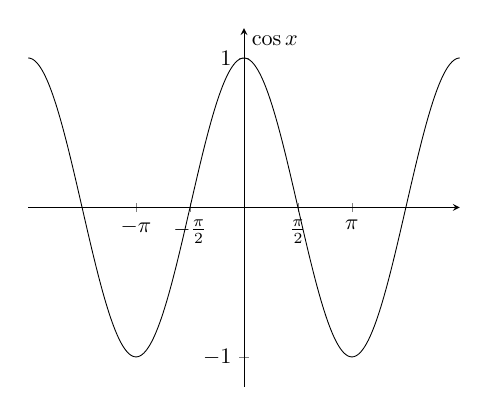
\begin{tikzpicture}[scale=0.8]
\begin{axis}[axis x line=middle,axis y line=middle,
		xtick={-180,-90,90,180},xticklabels={$-\pi$,$-\frac{\pi}{2}$,$\frac{\pi}{2}$,$\pi$},
		ytick={-1,1},
		xlabel={},ylabel={$\cos x$},
		samples=1000,
		xmin=-360,xmax=360,
		ymin=-1.2,ymax=1.2]
\addplot[domain=-360:360]{cos(x)};
\end{axis}
\end{tikzpicture}
\qquad
\begin{tikzpicture}[scale=0.8]
\begin{axis}[axis x line=middle,axis y line=middle,
		xtick={},ytick={1},
		xlabel={},ylabel={$\cosh x$},
		samples=1000,
		xmin=-5,xmax=5,
		ymin=-0.2,ymax=10]
\addplot[domain=-5:5]{(e^x + e^(-x))/2};
\end{axis}
\end{tikzpicture}
\end{center}

But in the complex plane, $\cosh$ is just a composition of $\cos$ and its $\displaystyle \frac{\pi}{2}$ rotation, i.e. $\cosh z = \cos iz$ and similarly $\sinh z = \sin iz.$

\begin{thm}[Properties of exponential]
\ \\
\begin{enumerate}
    \item $e^{z+w}=e^z e^w\qquad \forall z,w\in \mathbb C$
    \item $e^z\neq 0\qquad \forall z\in \mathbb C$
    \item $e^z=1 \Leftrightarrow z=2k\pi i,\ k\in \mathbb Z$
    \item $e^z=-1 \Leftrightarrow z=(2k+1)\pi i,\ k\in \mathbb Z$
\end{enumerate}
\end{thm}

\subsection{Argument and Log}
We can write $z$ as $|z|e^{i\theta}$. Let $z_1 z_2 \neq 0$, then
\[
z_1=z_2 \Leftrightarrow |z_1|e^{i\theta_1}=|z_2|e^{i\theta_2} \Leftrightarrow \left\{ \begin{aligned} |z_1|&=|z_2| \\ \theta_1-\theta_2 &= 2\pi k,\ k\in \mathbb Z \end{aligned} \right.
\]
So we define the function $\arg:\mathbb C\backslash\{0\} \rightarrow \{\text{subsets of }\mathbb R\}$ by
\[
z\mapsto \{\theta+2\pi k,\ k\in\mathbb Z\}.
\]
Note that $\arg$ is a \textit{multivalued} or \textit{set-valued} function.
\begin{prop}[Properties of argument]
\begin{enumerate}
    \item $\arg(\alpha z) = \arg (z)$ for $\alpha >0$
    \item $\arg(\alpha z) = \pi + \arg (z)$ for $\alpha <0$
    \begin{itemize}
        \item To see this note that $\alpha = (-\alpha)(-1) = |\alpha|e^{i\pi}$
    \end{itemize}
    \item $\arg \left(\frac1z\right) = -\arg (z)$
    \item $\arg(\overline{z}) = -\arg (z)$
    \item $\arg (zw) = \arg(z)+\arg(w)$
\end{enumerate}
\end{prop}
We can see there's much unnecessary ambiguity of $\arg$, so we define a single valued function related to it, called principal argument:
\[
\Arg (z) = (-\pi, \pi] \cap \arg (z)
\]
Note that $\Arg$ is not analytic in $\mathbb C\backslash\{0\}$:
\[
\begin{aligned}
\lim_{\varepsilon\downarrow 0}\Arg \left(e^{i(\pi-\varepsilon)} \right) &= \pi \\
\lim_{\varepsilon\downarrow 0}\Arg \left(e^{i(\pi+\varepsilon)} \right) &= -\pi ,
\end{aligned}
\]
but
\[
\lim_{\varepsilon \downarrow 0} \left|e^{i(\pi-\varepsilon)}-e^{i(\pi+\varepsilon)}\right|=0.
\]
\begin{center}
\begin{tikzpicture}
\draw[->] (-2,0) -- (2,0)node[anchor=north]{$\Re$};
\draw[->] (0,-2) -- (0,2)node[anchor=west]{$\Im$};
\draw[->] (0,0) -- (-1.5,0.5)node[anchor=south west]{$\pi-\varepsilon$};
\draw[->] (0,0) -- (-1.5,-0.5)node[anchor=north west]{$\pi+\varepsilon$};
\end{tikzpicture}
\end{center}
Now we would like to find $w:e^w=z.$ We know
\[
e^w = |z|e^{i\theta} = e^{\log |z| + i\arg (z)},
\]
so define $\log:\mathbb C\backslash \{0\} \rightarrow \{\text{subsets of }\mathbb C\}$ by $z\mapsto \log z = \Log |z|+i\arg (z)$ where $\Log$ is logarithm of $\mathbb R^+.$ Similar to $\arg$, we have a single value version $z\mapsto \Log(z) = \Log|z|+i \Arg(z)$.

Unfortunately we have a clash of notations of real logarithm and complex principal logarithm.
\begin{prop}[Properties of logarithm]
\begin{enumerate}
    \item $\log(zw) = \log z+ \log w$
    \item $\log z^{-1} = \log z$
\end{enumerate}
\end{prop}
Similarly $\Log$ is not analytic in $\mathbb C\backslash\{0\}$: for any $x<0$,
\[
\begin{aligned}
\lim_{\varepsilon\downarrow 0} \Log (x+ i\varepsilon)&=\log |x|+i\pi \\
\lim_{\varepsilon\downarrow 0} \Log (x- i\varepsilon)&=\log |x|-i\pi ,
\end{aligned}
\]
so it's not continuous at $\{x<0\}$.

\begin{center}
\begin{tikzpicture}
\draw[->] (-2,0) -- (2,0)node[anchor=north]{$\Re$};
\draw[->] (0,-2) -- (0,2)node[anchor=west]{$\Im$};
\draw[dashed] (-1.5,0.5)node{\textbullet} node[anchor=south]{$x+i\varepsilon$} -- (0,0.5);
\draw[dashed] (-1.5,-0.5)node{\textbullet} node[anchor=north]{$x-i\varepsilon$} -- (0,-0.5);
\end{tikzpicture}
\end{center}

But we see that $\Log$ is analytic on $\mathbb C \backslash \{ x\leq 0 \}$ by checking Cauchy–Riemann equations. (This is called a ``branch cut''.) Now we can apply calculus:
\[
\begin{aligned}
e^{\Log z} &= z \\
\left(e^{\Log z}\right)' = z' &= 1 = (\Log z)' e^{\Log z} = (\Log z)' z
\end{aligned}
\]
so $\displaystyle (\Log z)'=\frac1z$.

If $\alpha \in \mathbb C,\ z\neq 0$, we define
\[
z^\alpha := e^{\alpha \log z} = e^{\alpha \log |z| + \alpha i \arg (z)}
\]
which is set-valued. If $\alpha \in \mathbb Z$ then $z\mapsto z^\alpha$ is single-valued:
\[
e^{i\alpha \arg(z)} = e^{i (\alpha \theta+2\pi \underbrace{k \alpha}_{\in\mathbb Z},\ k\in \mathbb Z)} = e^{i\alpha \theta} ,
\]
and if $\alpha = \pm \frac{p}{q},\ p,q\in \mathbb N$, then $z^\alpha$ consists of at most $q$ elements:
\[
\left\{e^{\alpha \Log |z|} e^{2\pi i \alpha k}:0\leq k\leq q-1\right\},
\]
and in particular we have the $q$-th roots of unity
\[
1^{\frac{1}{q}} = \left\{e^{2\pi i \frac{k}{q}}:0\leq k\leq q-1\right\}.
\]

\begin{center}
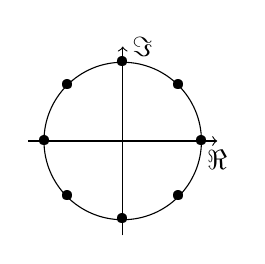
\begin{tikzpicture}
\draw[->] (-1.2,0) -- (1.2,0)node[anchor=north]{$\Re$};
\draw[->] (0,-1.2) -- (0,1.2)node[anchor=west]{$\Im$};
\draw (0,0) circle (1);
\draw (0,1)node{\textbullet};
\draw (0.707,0.707)node{\textbullet};
\draw (1,0)node{\textbullet};
\draw (0.707,-0.707)node{\textbullet};
\draw (0,-1)node{\textbullet};
\draw (-0.707,-0.707)node{\textbullet};
\draw (-1,0)node{\textbullet};
\draw (-0.707,0.707)node{\textbullet};
\end{tikzpicture}
\end{center}
\subsection{Complex integration, contour integrals}
\begin{defn}
$f:[a,b] \rightarrow \mathbb C$ is \textit{integrable} if $\Re f,\Im f:[a,b]\rightarrow \mathbb R$ are integrable. Then
\[
\int_a^b f := \int_a^b \Re f + i \int_a^b \Im f \qquad \in \mathbb C .
\]
\end{defn}
\begin{prop}[Properties of complex integration]
\begin{enumerate}
    \item Linearity: $\alpha,\beta \in \mathbb C,\ f,g:[a,b]\rightarrow \mathbb C$ integrable, then
    \[
    \int_a^b (\alpha f+\beta g) = \alpha \int_a^b f + \beta \int_a^b g
    \]
    \item Interchangeability of conjugation and integration:
    \[
    \overline{\int_a^b f} = \int_a^b \overline{f}
    \]
    \item Triangle inequality:
    \[
    \left|\int_a^b f \right| \leq \int_a^b |f|
    \]
\end{enumerate}
\end{prop}
\begin{proof}[Check]
\begin{enumerate}
    \item Let $\alpha = \mu + i\nu,\ f=u+iv$, then
    \[
    \alpha f = (\mu u-\nu v) + i (\mu v+\nu u).
    \]
    By definition and linearity of Riemann integral,
    \[
    \begin{aligned}
    \int_a^b \alpha f &= \mu \int_a^b u - \nu \int_a^b v + i \left( \mu \int_a^b v + \nu\int_a^b u \right) \\
    &= (\mu + i\nu ) \int_a^b u + i (\mu + i\nu ) \int_a^b v \\
    &= (\mu + i\nu ) \int_a^b (u+iv) \\
    &= \alpha \int_a^b f .
    \end{aligned}
    \]
    \item Left as an exercise.
    \item We know
    \[
    \int_a^b f = \left| \int_a^b f \right| e^{i\theta} \qquad \text{for some }\theta \in \mathbb R.
    \]
    So
    \[
    \left| \int_a^b f \right| = e^{-i\theta} \int_a^b f = \int_a^b \left(e^{-i\theta} f\right).
    \]
    Let $e^{-i\theta} f=u+iv$, then
    \[
    \int_a^b \left(e^{-i\theta} f\right) = \int_a^b u + i\int_a^b v
    \]
    but this is real, so $\int_a^b v=0.$ We can therefore use the triangle inequality for real and conclude that
    \[
    \int_a^b u \leq \int_a^b |u| \leq \int_a^b \sqrt{u^2+v^2} \int_a^b \left| e^{-i\theta} f\right| = \int_a^b |f|.
    \]
\end{enumerate}
\end{proof}

A more important aim is to define integral for $f:\mathbb C \rightarrow \mathbb C$. Such functions can be viewed as vector fields on $\mathbb R^2$, suggesting we can borrow the idea of line integral: $\displaystyle \int_\Gamma f \ \mathrm d z$ where $\Gamma$ is an oriented curve in $\mathbb C$. We need some terminology.
\begin{notation}
\begin{enumerate}
    \item $\gamma:[a,b]\rightarrow \mathbb C$ denotes a $C^1$ map called a \textit{parameterised curve}.
    \item $\Gamma = \gamma([a,b]) \subset \mathbb C$, this is an unparameterised curve, the equivalence class of maps from $\mathbb R$ to $\mathbb C$: $\gamma_1 \sim \gamma_2$ if $\text{Im } \gamma_1=\text{Im } \gamma_2$ .
    \item If $\Gamma$ is oriented, then $-\Gamma$ coincides with $\Gamma$ as a subset of $\mathbb C$, but has the opposite orientation
    \item Shorthand:
    \[
    \int_\Gamma f(z) \ \mathrm d z = \int_\Gamma f \ \mathrm d z = \int_\Gamma f .
    \]
    We use $\int_\gamma f$ to emphasise parameterisation.
\end{enumerate}
\end{notation}
\begin{remark}
For orientation to make sense, it is sufficient for $\gamma$ to be regular if $\gamma'\neq 0$ (you have tangent vector everywhere)
\end{remark}

\begin{defn}
Let $\Gamma \subset \mathbb C$ be oriented and $\gamma:[a,b]\rightarrow \mathbb C$ its parameterisation. Define
\[
\int_\Gamma f := \int_a^b f(\gamma(t)) \overbrace{\gamma'(t) \ \mathrm d t}^{``\mathrm d r\text{''}} .
\]
If $\Gamma$ is piecewise $C^1$, i.e. $\Gamma = \bigcup \Gamma_i$ where $\Gamma_i$'s are almost disjoint, then
\[
\int_\Gamma f := \sum_{k=1}^n \int_{\Gamma_k} f .
\]
\end{defn}
Standard properties of Riemann integrals like linearity and additivity hold.

\begin{lemma}[Representation invariance]
\begin{enumerate}
    \item \[
    \int_{-\gamma} f = -\int_\gamma f
    \]
    (If $\gamma:[a,b]\rightarrow \mathbb C$, then $-\gamma=\gamma (a+b-\cdot )$ (shift by $a+b$ then change sign)
    \item If $\gamma:[a,b]\rightarrow \mathbb C$ and $\phi:[\tilde{a},\tilde{b}]\rightarrow[a,b]$ is bijective, increasing and $C^1$, then
    \[
    \int_\gamma = \int_{\gamma \circ \phi} f
    \]
    ($\phi$ is an orient-preserving reparameterisation)
\end{enumerate}
\end{lemma}
\begin{remark}
\begin{enumerate}
\item By analogy with multivariable calculus we can define
\[
\int_\Gamma |f| |\mathrm d z| := \int_a^b |f(\gamma(t))| \cdot |\gamma'(t)| \ \mathrm d t
\]
Notice that if $f=1$, and write $\gamma(t)=x(t)+i y(t)$, then the above integral is
\[
\int_a^b \sqrt{x'^2(t)+y'^2(t)} \ \mathrm d t
\]
so it's just the Euclidean length of $\Gamma$. Hence
\[
\begin{aligned}
\left| \int_\Gamma f \ \mathrm d z \right| &= \left| \int_a^b f(\gamma(t)) \gamma'(t) \ \mathrm d t \right| \leq \int_a^b |f(\gamma(t))| \cdot |\gamma'(t)| \ \mathrm d t \\&\leq \underset{z\in \Gamma}{\sup} |f(z)| \int_a^b |\gamma'(t)| \ \mathrm d t = \underset{\Gamma}{\sup}|f| \cdot \text{length of } \Gamma 
\end{aligned}
\]
\item We can define
\[
\int_\Gamma f \ \mathrm d \overline{z} := \int_a^b f(\gamma(t)) \cdot \overline{\gamma '(t)} \ \mathrm d t ,
\]
but we will be mostly interested in
\[
\int_\Gamma f \ \mathrm d z
\]
where $f$ is analytic in an open subset $\Omega \subset \mathbb C$ and $\Gamma \in \Omega$ is an oriented curve. If we start considering all the versions of integrals we have listed here, we would end up reproducing theory of line integrals over vectors fields in $\mathbb R^2$. So by looking at the integral above, we specify on a very special class of vector fields, and this speciality comes from analyticity.
\end{enumerate}
\end{remark}

\begin{example}
\begin{enumerate}
\item Consider
\[
\int_{\Gamma=\partial \mathbb B_R(0)} z^n \ \mathrm d z,\qquad n\in \mathbb Z
\]
where $\partial \mathbb B_R(0)$ is circle of radius $R$, centred at origin and oriented counterclockwise. We parameterise it by
\[
\gamma (t) = Re^{it},\ t\in [0,2\pi].
\]
Then by definition,
\[
\begin{aligned}
\int_\Gamma z^n \ \mathrm d z &= \int_0^{2\pi} \left(Re^{it}\right)^n \cdot i Re^{it} \ \mathrm d t = i R^{n+1} \int_0^{2\pi} e^{i(n+1)} \ \mathrm d t \\&= i R^{n+1} \underbrace{\int_0^{2\pi} (\cos (n+1) t+ i\sin (n+1) t) \ \mathrm d t}_{0\text{ unless }n+1=0} \\
&= i R^{n+1} \delta_{n,-1} \int_0^{2\pi} 1 \ \mathrm d t \\
&= 2\pi i \delta_{n,-1},
\end{aligned}
\]
which doesn't depend on $R$!
\item From the above we can consider the exponential integrated on the same $\Gamma$; by its uniform convergence we can swap integral and infinite sum:
\[
\int_\Gamma e^z \ \mathrm d z = \int_\Gamma \sum_{n=0}^\infty \frac{z^n}{n!} \ \mathrm d z = \sum_{n=0}^\infty \frac{1}{n!} \int_\Gamma z^n \ \mathrm d z = \sum_{n=0}^\infty \frac{1}{n!} 2\pi i \delta_{n,-1} = 0.
\]
\item Consider
\[
\int_\Gamma \frac{e^z}{z^{k+1}} \ \mathrm d z,\qquad k\in \mathbb N_0.
\]
We rewrite
\[
\begin{aligned}
\int_\Gamma \sum_{n=0}^\infty \frac{1}{n!} z^{n-1-k} \ \mathrm d z &= \sum_{n=0}^\infty \frac{1}{n!} \int_\Gamma z^{n-1-k} \ \mathrm d z \\&= \sum_{n=0}^\infty \frac{1}{n!} 2\pi i \delta_{n-1-k,-1} \\&= 2\pi i \sum_{n=0}^\infty \frac{1}{n!} \delta_{n,k} = 2\pi i \frac{1}{k!} .
\end{aligned}
\]
\end{enumerate}
Note that $\frac{1}{k!}$ is the $k$-th term of Taylor of exponential at 0. We are integrating by differentiating. Also, take $k=0$, we are integrating $\frac{e^x}{x}$ whose antiderivative (called exponential integral, a special function) is not expressible. We now can do something beyond Fundamental theorem of calculus.
\end{example}
\begin{example}
\[
I_k = \int_{\partial \mathbb B_R(1+i)} z^k \ \mathrm d z,\qquad k\in \mathbb N_0,\ R>0 .
\]
We start with parameterising the circle by
\[
\gamma = (1+i) + Re^{it},\qquad t\in [0,2\pi],
\]
so by definition
\[
\begin{aligned}
I_k &= \int_0^{2\pi} \underbrace{\left(1+i+ Re^{it} \right)^k}_{z(\gamma)} \underbrace{i Re^{it}}_{\gamma '(t)} \ \mathrm d t \\
&= \int_{\partial \mathbb B_R(0)} (1+i+w)^k \ \mathrm d w \qquad \text{change of variables} \\
&= \sum_{n=0} ^k \binom{k}{n} (1+i)^{k-n} \int_{\partial \mathbb B_R(0)} w^n \ \mathrm d w = 0. \qquad \text{by binomial and previous example}
\end{aligned}
\]
\end{example}

\begin{thm}[Complex FTC, or line integrals of conservative fields]
Let $F:\Omega \rightarrow \mathbb C$ be analytic such that $F'=f$ is continuous and $\gamma:[a,b]\rightarrow \Omega$ be an oriented $C^1$ curve in $\Omega$. Then
\[
\int_\gamma f \ \mathrm d z = F(\gamma(b))-F(\gamma(a)),
\]
i.e. integral only depends on end points.
\end{thm}
\begin{proof}
\[
\begin{aligned}
\int_\gamma f \ \mathrm d z &= \int_a^b f(\gamma(t)) \gamma '(t) \ \mathrm d t = \int_a^b F'(\gamma(t)) \gamma'(t) \ \mathrm d t \\&= \int_a^b \frac{\mathrm d}{\mathrm d t} F(\gamma(t)) \ \mathrm d t \qquad \text{chain rule} \\&=F(\gamma(b))-F(\gamma(a)). \qquad \text{usual FTC}
\end{aligned}
\]
\end{proof}
\begin{remark}
$\Omega$ doesn't have to be simply connected.
\end{remark}

\subsubsection{Link with multivariable calculus}
Let $r:[a,b]\rightarrow \mathbb R^2$ be a curve in $\mathbb R^2$, $\underline v: \mathbb R^2\rightarrow \mathbb R^2$ be a vector field. If $C=\text{Im }r$ is closed, then 
\[
\int_C \underline v \cdot \mathrm d r = \int_a^b \underline v(r(t)) \cdot r'(t) \ \mathrm d t
\]
is called the circulation of $\underline v$ around $C$.

Now let $\Omega\subset \mathbb R^2$ be a regular domain (open, bounded, with piecewise $C^1$ boundary) which is positively oriented: meaning $N(t) = r'(t) \times e_z$ is outward normal. (We are thinking 2-d as a subspace of 3-d, $e_z$ is the unit vector pointing from the board toward the viewers).

The most important particular case, from which we will build everything, is $\Omega = \partial \gamma$ where $\gamma$ is simple closed curve oriented counterclockwise.

Explicitly, if $r'(t) = (x'(t),y'(t),0)$ and $e_z = (0,0,1)$, then
\[
N(t) = r'(t) \times e_z = (y'(t),-x'(t),0).
\tag{$\ast$}
\]
If $\Omega$ is positively oriented in this sense, then flux of $\underline u$ through $\partial \Omega$ is
\[
\int_{\partial \Omega} \underline u \cdot N \ \mathrm d t = \sum \int_{a_i}^{b_i} \underline u (\gamma(t)) N(t) \ \mathrm d t
\]
where the sum is over connect components of $\partial \Omega$.

Let $\Omega \subset \mathbb R^2$ be regular, positively oriented. Then
\[
\int_\Omega \nabla \times \underline u \ \underbrace{\mathrm d x \ \mathrm d y}_{\text{area element}} = \int_{\partial \Omega} \underline u \cdot \mathrm d  r
\]
(Green's theorem) and similarly
\[
\int_\Omega \nabla \cdot \underline u \ \mathrm d x \ \mathrm d y = \int_{\partial \Omega} \underline u \cdot N \ \mathrm d t
\]
(Divergence/Gauss's theorem).

\begin{remark}
$f:=u+iv: \Omega \rightarrow \mathbb C$. Let $\gamma:[a,b]\rightarrow \Omega$ be a curve. Consider
\[
\begin{aligned}
\int_\gamma f \ \mathrm d z &= \int_a^b (u+iv) (\gamma'_1+i \gamma'_2) = \int_a^b (u\gamma'_1 -v\gamma'_2) +i \int_a^b (v\gamma'_1 + u\gamma'_2) \\&=\int_a^b (u,-v) \cdot \underbrace{(\gamma'_1,\gamma'_2)}_{\gamma'(t)} + i\int_a^b (u,-v) \cdot \underbrace{(\gamma'_2,-\gamma'_1)}_{N(t)} \qquad \text{by ($\ast$) above} \\
&= \text{circulation of }\underline f + i \text{ flux of }\underline f
\end{aligned}
\]
where $\underline f$ is a vector field built out of $f$ which is written by $(u,-v):\mathbb R^2\rightarrow \mathbb R^2$.
\end{remark}
\begin{thm}[Cauchy's]
$\Omega \subset \mathbb C$ is open, simply connected. $f:\Omega \rightarrow \mathbb C$ is analytic, $\gamma \subset \Omega$ is a $C^1$ closed, simple curve (i.e. a contour). Then
\[
\int_\gamma f \ \mathrm d z=0.
\]
\end{thm}
\begin{proof}
Let $D\subset \mathbb C$ be the domain bounded by $\gamma$ (the interior of $\gamma$). $D$ is then regular and $\partial D=\gamma$. $D$ indeed exists by Jordan curve theorem. We claim $D\subset \Omega$. Indeed, suppose $D\not\subset \Omega$. Then $\exists z_0 \in D:z_0 \not\in \Omega$. Since $\Omega$ is simply connected, there is a family of curves $(\gamma_t)_{t\in [0,1]}$, a continuous deformation of $\gamma : \gamma_0=\gamma, \gamma_1=z_1 \in \Omega$ and $\gamma_t \subset \Omega \ \forall t\in [0,1]$. Since $z_0\neq z_1$, $\exists \varepsilon >0: z_0$ is in the exterior of $\gamma_{1-\varepsilon}$. By Intermediate value theorem, $\exists \tau \in [0,1]:z_0\in \gamma_\tau \subset \Omega$, a contradiction.

\begin{center}
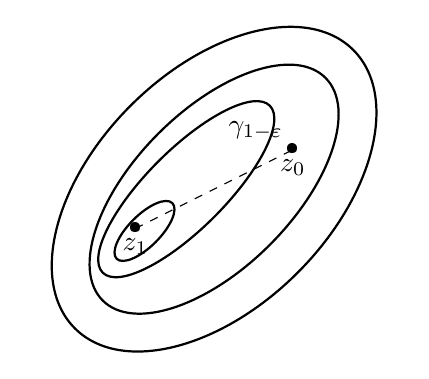
\begin{tikzpicture}
\draw[rotate around={45:(0,0)}][thick] (0,0) ellipse (2.5cm and 1.5cm);
\draw[rotate around={45:(0,0)}][thick] (0,0) ellipse (2cm and 1cm);
\draw[rotate around={45:(0,0)}][thick] (-0.25,0.25) ellipse (1.5cm and 0.5cm);
\draw[rotate around={45:(0,0)}][thick] (-1,0.25) ellipse (0.5cm and 0.2cm);
\draw[dashed] (-1,-0.5)node{\textbullet} node[anchor=north]{$z_1$} -- (1,0.5)node{\textbullet}node[anchor=north]{$z_0$} node[anchor=south east]{$\gamma_{1-\varepsilon}$};
\end{tikzpicture}
\end{center}

So $f$ is analytic in $D\cup \gamma$, and
\[
\begin{aligned}
\int_\gamma f \ \mathrm d z &= \text{circ}_\gamma (\underline f) +i \text{ flux}_\gamma (\underline f) \\ &= \int_D \nabla \times \underline f + i\int_D \nabla \cdot \underline f \qquad \text{Green's on first term, Gauss's on second} \\
&=\int_D \left( -\frac{\partial v}{\partial x}-\frac{\partial u}{\partial y}\right)+ i\int_D \left(\frac{\partial u}{\partial x}-\frac{\partial v}{\partial y} \right) \\&=0+i\cdot 0 \qquad \text{Cauchy–Riemann} \\&= 0.
\end{aligned}
\]
\end{proof}
\begin{remark}
\begin{enumerate}
    \item Analytic functions give rise to very special vector fields $\underline f$ with both $\text{curl }\underline f$ and $\text{div }\underline f$ equal to zero.
    \item Consider $\int_{\partial \mathbb B_R(0)} z^{-1} \ \mathrm d z$. $z^{-1}$ is analytic in $\mathbb C \backslash \mathbb B_R(0) \ \forall R>0$, which is not simply connected, in other words, we cannot deform a circle to a point since the hole won't let us. And indeed we know the integral is $2\pi i \neq 0$.
\end{enumerate}
\end{remark}
It turns out that Cauchy's theorem is a very powerful tool for computing contour integrals.
\begin{thm}[Contour deformation]
$\Omega \subset \mathbb C$ positively oriented, regular such that $\partial \Omega = \gamma_1 \cup \gamma_2$ and $\gamma_1 \cap \gamma_2 = \varnothing$ and $\gamma_i$'s are contours. Let $f:\Omega \cup \gamma_1 \cup \gamma_2$ be analytic. Then
\[
\int_{\gamma_1} f + \int_{\gamma_2} f = 0.
\]
Equivalently, 
\[
\int_{\gamma_1} f = \int_{-\gamma_2} f.
\]
(Deforming the contour within in the region of analyticity does not change the integral of an analytic function.)
\end{thm}
\begin{proof}[Picturesque proof]
Parameterise $\gamma_i$ from $p_i$ and $\eta$ from $p_2$ to $p_1$. Note that $\Omega \backslash \eta$ is simply connected. So by Cauchy's theorem,
\[
\begin{aligned}
\int_{\partial (\Omega \backslash \eta)} f &= \int_{\gamma_2} f + \int_\eta f + \int_{\gamma_1} f + \int_{-\eta} f \\&= \int_{\gamma_1} f + \int_{\gamma_2} f \\&= 0.
\end{aligned}
\]

\begin{center}
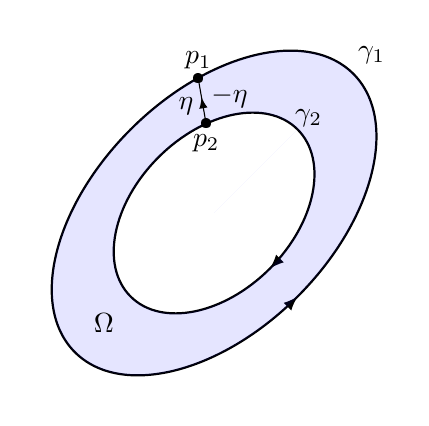
\begin{tikzpicture}
\draw[rotate around={45:(0,0)},name path=A,postaction={decoration={
    markings,
    mark = at position 0.75 with {\arrow{latex}}
    }, decorate}][thick] (0,0) ellipse (2.5cm and 1.5cm);

\draw[rotate around={45:(0,0)},name path=B,postaction={decoration={
    markings,
    mark = at position 0.75 with {\arrowreversed{latex}}
    }, decorate}][thick] (0,0) ellipse (1.5cm and 1cm);
\tikzfillbetween[of=A and B]{blue, opacity=0.1};
\node at (-1.4,-1.4) {$\Omega$};
\node at (2,2) {$\gamma_1$};
\node at (1.2,1.2) {$\gamma_2$};
\node at (-0.2,1.7) {\textbullet};
\node at (-0.2,1.7) [anchor=south]{$p_1$};
\node at (-0.1,1.125) {\textbullet};
\node at (-0.1,1.125) [anchor=north]{$p_2$};
\draw[postaction={decoration={
    markings,
    mark = at position 0.4 with {\arrowreversed{latex}}
    }, decorate}] (-0.2,1.7) -- (-0.1,1.125) node[pos=0.6,anchor=east]{$\eta$}node[pos=0.4,anchor=west]{$-\eta$};
\end{tikzpicture}
\end{center}
\end{proof}
\begin{remark}
\begin{enumerate}
    \item Terminology: given contour $\gamma$, $I(\gamma)$ denotes interior of $\gamma$ which is open, bounded subset of $\mathbb C$ and $\partial I(\gamma) = \gamma$, and $\overline{I(\gamma)} = I(\gamma) \cup \gamma$. $O(\gamma)$ denotes out outside of $\gamma$, which is equal to $\overline{I(\gamma)}^C$.
    \item We established before that
    \[
    \int_{\partial \mathbb B_R(0)} z^n \ \mathrm d z = 2\pi i \delta_{n,-1}.
    \]
    Now similarly, 
    \[
    \int_{\partial \mathbb B_R(a)} (z-a)^n \ \mathrm d z = 2\pi i \delta_{n,-1}.
    \]
    Fix $z\in \mathbb C$,
    \[
    \frac{1}{2\pi i}\int_\gamma \frac{1}{z-w} \ \mathrm d w = \left\{ \begin{aligned}
       &0 \qquad &z\in O(\gamma)\\
       &1 \qquad &z\in I(\gamma)
    \end{aligned} \right.
    \]
    since if $z\in O(\gamma)$ it's just Cauchy's theorem, but if $z\in I(\gamma)$ we can surround $z$ by a ball and deform $\gamma$ to the ball continuously, and by previous theorem the two integrals are the same, so it's $\frac{2\pi i}{2\pi i} =1.$
\end{enumerate}
\end{remark}

\begin{thm}
Let $\gamma \subset \mathbb C$ be a contour (oriented counterclockwise). Suppose $f$ is analytic in $\overline{I(\gamma)}$. Then $\forall z\in I(\gamma)$,
\[
f(z) = \frac{1}{2\pi i} \int_\gamma \frac{f(w)}{w-z} \ \mathrm d w,
\]
i.e. given analytic function and its values on a contour, we can give value of the function anywhere inside the contour.
\end{thm}
\begin{proof}
Note that $\displaystyle \frac{f(w)}{w-z}$ is analytic in $I(\gamma)\backslash \mathbb B_R(z)$ where $R>0:\mathbb B_R(z) \subset I(\gamma)$, so

\[
\begin{aligned}
\frac{1}{2\pi i} \int_\gamma \frac{f(w)}{w-z} \ \mathrm d w&=\frac{1}{2\pi i} \int_{\partial \mathbb B_R(z)} \frac{f(w)}{w-z} \ \mathrm d w \\ &= \frac{1}{2\pi i} \int_{\partial \mathbb B_R(z)} \frac{f(z)}{w-z} \ \mathrm d w+\underbrace{\frac{1}{2\pi i} \int_{\partial \mathbb B_R(z)} \frac{f(w)-f(z)}{w-z} \ \mathrm d w}_{\text{error term}} \\&= f(z)+\frac{1}{2\pi i} \int_{\partial \mathbb B_R(z)} f'(z) +g_z(w) \ \mathrm d w
\end{aligned}
\]
where $|g_z(w)| \rightarrow 0$ as $|w-z|\rightarrow 0$, and since $R$ is arbitrarily small, 
\[
\begin{aligned}
\left|\frac{1}{2\pi i} \int_{\partial \mathbb B_R(z)} f'(z) +g_z(w) \ \mathrm d w\right| &= \frac{1}{2\pi} \int_{\partial \mathbb B_R(z)} |f'(z) + g_z(w) | |\mathrm d w| \\ &\leq \frac{1}{2\pi} \left( |f'(z)|+\underset{z\in \mathbb B_R(z)}{\sup} |g_z(w)| \right) 2\pi R \\&=0
\end{aligned}
\]
so the error term vanishes and we have what's desired.
\begin{center}
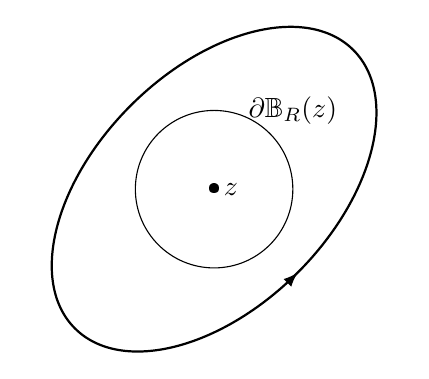
\begin{tikzpicture}
\draw[rotate around={45:(0,0)},postaction={decoration={
    markings,
    mark = at position 0.75 with {\arrow{latex}}
    }, decorate}][thick] (0,0) ellipse (2.5cm and 1.5cm);
\node at (0,0) [anchor=west]{$z$};
\node at (0,0) {\textbullet};
\node at (1,1) {$\partial \mathbb B_R(z)$};
\draw (0,0) circle[radius=1cm];
\end{tikzpicture}
\end{center}
\end{proof}

We can generalise this statement.
\begin{thm}
Let $\gamma \subset \mathbb C$ be a contour (oriented counterclockwise). Suppose $f$ is analytic in $\overline{I(\gamma)}$. Then $\forall z\in I(\gamma),\ \forall n\in \mathbb N_0$,
\[
f^{(n)}(z) = \frac{n!}{2\pi i} \int_\gamma \frac{f(w)}{(w-z)^{n+1}} \ \mathrm d w,
\]
i.e. the derivative of any order exists at any point where $f$ is analytic and we can differentiate by integrating.
\end{thm}
\begin{proof}[Shortcut proof]
$f$ is analytic at every $w\in \gamma$. Therefore $\exists \varepsilon(w) : f$ is analytic in $\mathbb B_{\varepsilon(w)} (w)$. Consider $\{\mathbb B_{\varepsilon(w)}(w)\}_{w\in \gamma}$, which is an open cover of $\gamma$, i.e. union of elements in this set is open and contains $\gamma$. Note that $\gamma$ is compact (closed, bounded), so by a theorem which will be proved in MA260, $\exists$ a finite subcover $\{\mathbb B_{\varepsilon(w_i)} (w_i)\}_{i=1}^N$ of $\gamma$. Let $\widetilde{\gamma}$ be a contour such that
\[
\widetilde{\gamma} \subset \left( \bigcup_{i=1}^N \mathbb B_{\varepsilon(w_i)} (w_i) \right) \cap O(\gamma).
\]
The following picture makes clear. The thick curve is $\gamma$, where $f$ is analytic, so we can exploit this fact and find an outside curve which is still in the ball-cover, and $f$ is analytic in $\widetilde{\gamma}$ and $I(\widetilde{\gamma})$.
\begin{center}
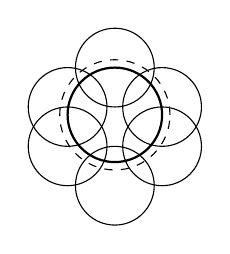
\begin{tikzpicture}
\draw (-0.1,0) circle (0.5cm);
\draw (-0.1,-0.5) circle (0.5cm);

\draw (0.5,-1) circle (0.5cm);

\draw (1.1,-0.5) circle (0.5cm);
\draw (1.1,0) circle (0.5cm);

\draw (0.5,0.5) circle (0.5cm);

\draw[thick] (0.5,-0.1) circle (0.6cm);
\draw[dashed] (0.5,-0.1) circle (0.7cm);
\end{tikzpicture}
\end{center}
Then by previous theorem
\[
f(z) =\frac{1}{2\pi i} \int_{\widetilde{\gamma}} \frac{f(w)}{w-z} \ \mathrm d w ,
\]
so
\[
\begin{aligned}
\frac{f(z+h)-f(z)}{h} &= \frac{1}{2h\pi i} \int_{\widetilde{\gamma}} \frac{f(w)}{w-z-h}-\frac{f(w)}{w-z} \ \mathrm d w \\&=\frac{1}{2h\pi i} \int_{\widetilde{\gamma}} \frac{f(w)h}{(w-z-h)(w-z)} \ \mathrm d w \\&=\frac{1}{2\pi i} \int_{\widetilde{\gamma}} f(w) \frac{1}{(w-z)^2} \ \mathrm d w + \frac{1}{2\pi i} E_h,
\end{aligned}
\]
where
\[
\begin{aligned}
E_h &= \int_{\widetilde{\gamma}} f(w) \left(\frac{1}{(w-z-h)(w-z)} - \frac{1}{(w-z)^2} \right) \ \mathrm d w \\&=\int_{\widetilde{\gamma}} f(w) \frac{h}{(w-z)^2(w-z-h)} \ \mathrm d w \\&\underset{\text{for any }|h|<r}{=} h \int_{\partial \mathbb B_{2R}(z)} \frac{f(w)}{(w-z)^2 (w-z-h)} \ \mathrm d w
\end{aligned}
\]
where the integrand is uniformly bounded as $|w-z-h|\geq r$.
\begin{center}
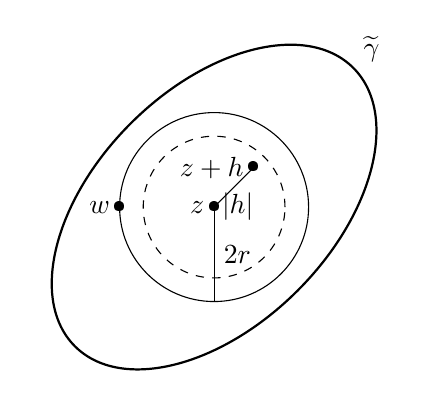
\begin{tikzpicture}
\draw[rotate around={45:(0,0)}][thick] (0,0) ellipse (2.5cm and 1.5cm);
\draw circle[radius=1.2cm] (0,0);
\draw (0,0) -- (0,-1.2)node[pos=0.5,anchor=west]{$2r$};
\draw (0,0)node{\textbullet} node[anchor=east]{$z$} -- (0.5,0.5)node{\textbullet} node[anchor=east]{$z+h$} node[pos=0.6,anchor=north]{$|h|$};
\draw[dashed] circle[radius=0.9cm] (0,0);
\node at (2,2) {$\widetilde{\gamma}$};
\node at (-1.2,0) {\textbullet};
\node at (-1.2,0) [anchor=east]{$w$};
\end{tikzpicture}
\end{center}

Therefore as $h\rightarrow 0$, $E_h$ vanishes. Hence
\[
f'(z) = \frac{1}{2\pi i} \int_{\widetilde{\gamma}} f(w) \frac{1}{(w-z)^2} \ \mathrm d w .
\]
Now, pick any $z\in I(\widetilde{\gamma})$,
\[
\begin{aligned}
\frac{f'(z+h)-f'(z)}{h} &= \frac{1}{2h\pi i} \int_{\widetilde{\gamma}} f(w) \left(\frac{1}{(w-z-h)^2}-\frac{1}{(w-z)^2} \right) \ \mathrm d w \\ &=\frac{1}{2\pi i} \int_{\widetilde{\gamma}} f(w) \frac{2(w-z)-h}{(w-z-h)^2(w-z)^2} \ \mathrm d w \\&= \frac{2}{2\pi i} \int_{\widetilde{\gamma}} \frac{f(w)}{(w-z)^3} \ \mathrm d w+E_h
\end{aligned}
\]
where we separate the integral to the target and error term $E_h$ by putting $h=0$. Then $E_h \rightarrow 0$ as $h\rightarrow 0$ similarly, so we have
\[
f''(z) = \frac{2}{2\pi i} \int_{\widetilde{\gamma}} \frac{f(w)}{(w-z)^3} \ \mathrm d w ,
\]
as desired. We proceed by induction to get the general result: $f''(z)$ exists $\forall z\in I(\widetilde{\gamma}) \Rightarrow f'$ is analytic in $I(\widetilde{\gamma}) \Rightarrow f'$ is analytic in $\overline{I(\gamma)}$. So we've proven that
\[
f\text{ analytic in }\overline{I(\gamma)} \Rightarrow f' \text{ analytic in }\overline{I(\gamma)}.
\]
Therefore $f^{(n)}$ is analytic in $\overline{I(\gamma)}$. So by Theorem 4.6.10,
\[
\begin{aligned}
f^{(n)}(z) &= \frac{1}{2\pi i} \int_\gamma \frac{f^{(n)} (w)}{w-z} \ \mathrm d w \\&= \frac{1}{2\pi i} \left(-\int_\gamma f^{(n-1)} (w) \frac{\partial}{\partial w} \frac{1}{w-z} \ \mathrm d w \right) \qquad \text{integration by parts} \\&= \frac{1}{2\pi i} \int_\gamma f^{(n-1)}(w) \frac{1}{(w-z)^2} \ \mathrm d w \\&= \frac{2}{2\pi i} \int_\gamma f^{(n-2)}(w) \frac{1}{(w-z)^3} \ \mathrm d w \qquad \text{integration by parts again} \\&= \cdots \qquad \text{again and again} \\&= \frac{n!}{2\pi i} \int_\gamma f(w)\frac{1}{(w-z)^{n+1}} \ \mathrm d w,
\end{aligned}
\]
as desired.
\end{proof}

\subsubsection{Consequences of Cauchy's theorem}
\begin{thm}[Taylor's theorem]
Let $f$ be analytic in $\mathbb B_R(a) \subset \mathbb C,\ R>0,\ a\in \mathbb C$. Then $\exists ! (c_n)_{n\geq 0} \subset \mathbb C:\forall z\in \mathbb B_R(a),$
\[
f(z) = \sum_{n=0}^\infty c_n (z-a)^n,
\]
moreover, 
\[
c_n = \frac{1}{2\pi i} \int_\gamma \frac{f(w)}{(w-z)^{n+1}} \ \mathrm d w = \frac{f^{(n)}(a)}{n!}
\]
where $\gamma \subset \mathbb B_R(a)$ is any contour such that $a\in I(\gamma)$.

(Informally, if $f$ is analytic at $a$ then its Taylor series has a positive radius of convergence and is equal to $f$ within the corresponding ball.)
\end{thm}
\begin{proof}
We know $\forall z\in \mathbb B_R(a),\ \exists \gamma \in (|z-a|,R):\mathbb B_r(a) \subset \mathbb B_R(a)$.
\begin{center}
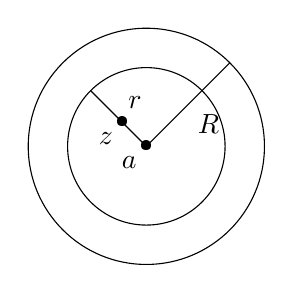
\begin{tikzpicture}
\draw circle[radius=1cm] (0,0);
\draw circle[radius=1.5cm] (0,0);
\node at (0,0) {\textbullet};
\node at (0,0) [anchor=north east] {$a$};
\node at (-0.3,0.3) {\textbullet};
\node at (-0.3,0.3) [anchor=north east] {$z$};
\draw (0,0) -- (-0.707,0.707) node[pos=0.5,anchor=south west]{$r$};
\draw (0,0) -- (1.06,1.06) node[pos=0.5,anchor=north west]{$R$};
\end{tikzpicture}
\end{center}

Since $f$ is analytic in $\overline{\mathbb B_r(a)}$, by Theorem 4.6.10 we have
\[
\begin{aligned}
f(z) &= \frac{1}{2\pi i} \int_{\partial \mathbb B_r(a)} \frac{f(w)}{w-z} \ \mathrm d w\\
&= \frac{1}{2\pi i} \int_{\partial \mathbb B_r(a)} \frac{f(w)}{w-a} \frac{w-a}{w-z} \ \mathrm d w \\
&=\frac{1}{2\pi i} \int_{\partial \mathbb B_r(a)} \frac{f(w)}{w-a} \frac{1}{1-\frac{z-a}{w-a}} \ \mathrm d w.
\end{aligned}
\]
Note that
\[
\left| \frac{z-a}{w-a} \right| = \frac{|z-a|}{r} <1.
\]
So
\[
\frac{1}{1-\frac{z-a}{w-a}} = \sum_{n=0}^\infty \left( \frac{z-a}{w-a}\right)^n
\]
which converges uniformly with respect to $w$ by the $M$-test. This means we can interchange integration and summation and we have
\[
\begin{aligned}
f(z) &= \frac{1}{2\pi i} \int_{\partial \mathbb B_r(a)} \frac{f(w)}{w-a} \sum_{n=0}^\infty \left( \frac{z-a}{w-a}\right)^n \ \mathrm d w. \\
&= \frac{1}{2\pi i} \sum_{n=0}^\infty \int_{\partial \mathbb B_r(a)} \frac{f(w)}{(w-a)(w-a)^n}\ \mathrm d w \ (z-a)^n.
\end{aligned}
\]
By Theorem 4.6.11 this is what's desired. $\partial \mathbb B_r(a)$ can be replaced with any $\gamma$ encompassing $a$ by Contour deformation theorem ($\gamma \subset \mathbb B_R(a)$).

For uniqueness, suppose
\[
f(z) = \sum_{n=0}^\infty b_n (z-a)^n \quad \forall z\in \mathbb B_{\rho}(a) \text{ for some }\rho>0
\tag{$\ast$}
\]
then the right hand side of $(\ast)$ converges uniformly in $\overline{\mathbb B_{\rho'} (a)} \ \forall \rho '<\rho$. So we can differentiate term by term for any $z\in \mathbb B_{\rho'} (a)$. By Theorem 3.3.4, $b_n=\frac{1}{n!} f^{(n)}(a)=c_n$.
\end{proof}

\begin{example}
Let $f:z\mapsto (1+z)^a$ in $\mathbb B_1(0)$ and $a\in \mathbb C$ fixed. We know $f(z) = e^{a \Log (1+z)}$ is analytic in $\mathbb B_1(0)$ since $z\mapsto e^z$ is entire and $\Log(1+z)$ is analytic in $\mathbb C \backslash \{x\leq -1\}$. So for any $\rho <1$,
\[
(1+z)^a = \sum_{n=0}^\infty z^n \frac{1}{2\pi i} \int_{\partial \mathbb B_\rho (0)} \frac{(1+w)^a}{w^{n+1}} \ \mathrm d w.
\]
If we denote $\frac{1}{2\pi i} \int_{\partial \mathbb B_\rho (0)} \frac{(1+w)^a}{w^{n+1}} \ \mathrm d w$ by $c_n$ we have
\[
\begin{aligned}
c_n&=\frac{1}{2\pi i} \frac{1}{-n} \int \left(w^{-n}\right)' (1+w)^a \ \mathrm d w \\
&=\frac{1}{2\pi i} \frac{1}{n!} \int w^{-n}a (1+w)^{a-1} \ \mathrm d w \qquad \text{integration by parts} \\
&= \frac{1}{2\pi i} \frac{a}{n} \int_{\partial \mathbb B_\rho (0)} w^{-n} (1+w)^{a-1} \ \mathrm d w \\
&=\frac{1}{2\pi i} \frac{a(a-1)}{n(n-1)} \int_{\partial \mathbb B_\rho (0)} w^{-(n-1)} (1+w) ^{a-2} \ \mathrm d w \qquad \text{by parts again} \\ 
&=\frac{1}{2\pi i } \prod_{k=0}^{n-1} \frac{a-k}{n-k} \int \frac{(1+w)^{a-n}}{w} \ \mathrm d w \\
&= \prod_{k=0}^{n-1} \frac{a-k}{n-k}\int \frac{(1+w)^{a-n}}{w} \ \frac{\mathrm d w}{2\pi i}.
\end{aligned}
\]
We know $w\mapsto (1+w)^{a+n}$ is analytic at $w=0$. So
\[
\frac{(1+w)^{a-n}-1^{a-n}}{w} = \left((1+z)^{a-n}\right)'|_{z=0} + \varphi(w)
\]
where the error term $\varphi(w)\rightarrow 0$ as $w\rightarrow 0$. So
\[
\frac{1}{2\pi i} \int_{\partial \mathbb B_\rho (0)} \frac{(1+w)^{a-n}}{w} \ \mathrm d w = \underbrace{\frac{1}{2\pi i} \int \frac{1}{w} \ \mathrm d w}_{1} + \underbrace{\frac{1}{2\pi i} \int_{\partial \mathbb B_\rho (0)} (a-n) +\varphi(w) \ \mathrm d w}_{0},
\]
therefore
\[
c_n = \prod_{k=0}^{n-1} \frac{a-k}{n-k}=\frac{1}{n!} \prod_{k=0}^{n-1} (a-k).
\]
By above theorem, $\sum_{n=0}^\infty c_n z^n$ converges for any $|z|\leq \rho$ where $\rho \in (0,1)$, so radius of convergence $R\geq 1$.
\end{example}

\begin{thm}[Liouville's theorem]
Let $f:\mathbb C\rightarrow \mathbb C$ be entire. If $f$ is bounded, then $f$ is constant.
\end{thm}
\begin{proof}
$f$ is bounded, meaning $\exists M>0:|f(z)|\leq M \ \forall z\in \mathbb C$. For any $z\in \mathbb C$, take $R>|z|$, 

\begin{center}
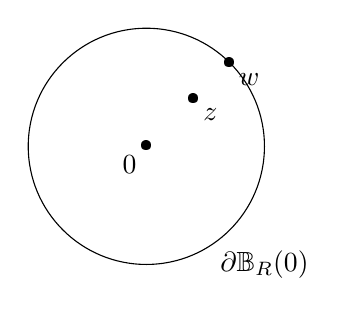
\begin{tikzpicture}
\draw circle[radius=1.5cm] (0,0);
\node at (0,0) {\textbullet};
\node at (0,0) [anchor=north east] {$0$};
\node at (0.6,0.6) {\textbullet};
\node at (0.6,0.6) [anchor=north west] {$z$};
\node at (1.5,-1.5) {$\partial \mathbb B_R(0)$};
\node at (1.05,1.05) {\textbullet};
\node at (1.05,1.05) [anchor=north west] {$w$};
\end{tikzpicture}
\end{center}
then
\[
f(0)=\frac{1}{2\pi i} \int_{\partial \mathbb B_R(0)} \frac{f(w)}{w} \ \mathrm d w
\]
and
\[
f(z)=\frac{1}{2\pi i} \int_{\partial \mathbb B_R(0)} \frac{f(w)}{w-z} \ \mathrm d w.
\]
To see $f$ is constant we need $f(z)-f(0)=0$. Indeed:
\[
\begin{aligned}
|f(z)-f(0)| &= \left|\frac{1}{2\pi i} \int_{\partial \mathbb B_R(0)} f(w) \left( \frac{1}{w-z}-\frac{1}{w}\right) \ \mathrm d w\right| \\
&= \frac{|z|}{2\pi} \left|\int_{\partial \mathbb B_R(0)} f(w) \frac{1}{(w-z)w} \ \mathrm d w \right| \\
&\leq \frac{|z|}{2\pi} \int_{\partial \mathbb B_R(0)} \frac{|f(w)|}{|w||w-z|} \ |\mathrm d w| \\
&\leq \frac{|z|}{2\pi} \int_{\partial \mathbb B_R(0)} \frac{M}{R(R-|z|)} \ |\mathrm d w| \\
&=\frac{|z|}{2\pi} \frac{M}{R(R-|z|)} 2\pi R \\
&= \frac{|z|M}{R-|z|}
\end{aligned}
\]
but since $f$ is entire, we can have $R$ as large as we want. Therefore $\frac{|z|M}{R-|z|}\rightarrow 0$ and therefore $f(z)=f(0)$.
\end{proof}

\begin{thm}[Fundamental theorem of algebra]
Let $p:\mathbb C\rightarrow \mathbb C$ a non-constant polynomial. Then $\exists a \in \mathbb C:p(a)=0$.
(Any complex non-constant polynomial has a root.)
\end{thm}
\begin{proof}[Proof by contradiction]
Suppose $p(z)\neq 0 \ \forall z\in \mathbb C$. Then $f:=\frac{1}{p}$ is analytic in $\mathbb C$, i.e. entire. Indeed, $z\mapsto p(z)$ is entire and $x\mapsto \frac{1}{x}$ is analytic when $x\neq 0$. Since $p$ is non-constant, $\exists n>0:p(z) =\sum_{k=0}^n c_k z^k$ where $c_i\neq 0$. So $|p(z)| \rightarrow \infty$ as $|z|\rightarrow \infty$. Then $\exists R>0:|p(z)|\geq 1 \ \forall |z| \geq R$. So $|f(z)| \leq 1 \ \forall |z| \geq R$. But for $|z| \leq R$, $f$ is also bounded, as an analytic hence continuous function on a closed bounded set. We conclude that $f$ is entire and bounded, so constant, hence $p$ is constant which is a contradiction.
\end{proof}
\begin{thm}
$f_n:\Omega \rightarrow \mathbb C,\ \Omega$ open, $n\geq 1$ are all analytic in $\Omega$. If $f_n \rightrightarrows f:\Omega \rightarrow \mathbb C$, then $f$ is analytic.
\end{thm}
\begin{proof}
$\forall z\in \Omega$, let $r>0$, pick small enough $\overline{\mathbb B_r(z)} \subset \Omega$. Since $f_n$ is analytic,
\[
f_n(z) = \frac{1}{2\pi i} \int_{\partial \mathbb B_r(z)} \frac{f_n(w)}{w-z} \ \mathrm d w
\]
so
\[
\begin{aligned}
f(z) &= \frac{1}{2\pi i} \lim_{n\rightarrow \infty} \int_{\partial \mathbb B_r(z)} \frac{f_n(w)}{w-z} \ \mathrm d w \\
&=\frac{1}{2\pi i} \int_{\partial \mathbb B_r(z)} \frac{f(w)}{w-z} \ \mathrm d w + \lim_{n\rightarrow \infty} E_n(z)
\end{aligned}
\]
where $E_n(z)$ is the error term (difference of the two). We know that by uniform convergence, $\forall \varepsilon >0,\ \exists N_\varepsilon: \forall n>N_\varepsilon,\ \underset{\Omega}{\sup} |f-f_n| <\varepsilon$, so
\[
\begin{aligned}
|E_n(z)| &\leq \frac{1}{2\pi} \int_{\partial \mathbb B_r(z)} \frac{|f_n(w)-f(w)|}{|w-z|} \ |\mathrm d w| \\
&< \frac{1}{2\pi r} \varepsilon \int_{\partial \mathbb B_r(z)} 1 \ |\mathrm d w| \\
&= \frac{1}{2\pi r} \varepsilon 2\pi r = \varepsilon,
\end{aligned}
\]
so $\lim_{n\rightarrow \infty} E_n(z)=0$, i.e.
\[
f(z)=\frac{1}{2\pi i} \int_{\partial \mathbb B_r(z)} \frac{f(w)}{w-z} \ \mathrm d w.
\]
Note that $f_n|_{\partial \mathbb B_r(z)} \rightrightarrows f|_{\partial \mathbb B_r(z)}$, so $f|_{\partial \mathbb B_r(z)}$ is continuous (on a closed bounded set), hence bounded. From the proof of Theorem 4.6.11 we know that $f'$ exists at every point $z\in \Omega$, i.e. $f$ is analytic.
\end{proof}
\subsubsection{Calculation of integrals over $\mathbb R$ using Cauchy's theorem}
\begin{defn}
Let $f$ be defined on a subset of $\mathbb C$. $f$ has a \textit{pole} of order $m\in \mathbb N$ at $a\in \mathbb C$ if $\exists$ a neighbourhood $U$ of $a:\forall z\in U\backslash \{a\}$,
\[
f(z) = \frac{c_{-m}}{(z-a)^m}+\frac{c_{-m+1}}{(z-a)^{m-1}}+\cdots+\frac{c_{-1}}{z-a}+\phi(z)
\]
where $\phi$ is analytic in $U$, $c_i \in \mathbb C$ are constants. Moreover, $c_{-1}$ is called the \textit{residue} of $f$ at a, $c_{-1}=\text{Res }f(a)$. $c_{-m} \neq 0$.
\end{defn}
Having a pole means the function is not defined at a certain point but on a neighbourhood of it, and we know that as we approach the point the function blows up at a rate quantified by the pole's order $m$ and described as a Laurent polynomial of the distance.
\begin{example}
Let $f:z\mapsto \frac{1}{z^2+a^2},\ a>0$. We claim $f$ has first order poles at $z=\pm ia$. Indeed,
\[
f(z) = \frac{1}{2i a } \left(\frac{1}{z-ia}-\frac{1}{z+ia} \right)
\]
and we can read off the pole $z=ia$, corresponding $\phi(z)=-\frac{1}{z+ia}$ and $\text{Res }f=\frac{1}{2ia}$ from the above and the definition. Similar (in fact symmetrically) for the other pole $z=-ia$.
\end{example}
\begin{thm}[Residue theorem]
Let $\gamma \subset \Omega$ be a contour oriented counterclockwise. Suppose $f$ is analytic in $\overline{I(\gamma)}\backslash \{z_1,\ldots,z_n\}$ where $z_i$'s are finitely many points living inside $I(\gamma)$. Moreover, suppose $f$ has poles at $z_1,\ldots,z_n$. Then
\[
\int_\gamma f(z) \ \mathrm d z = \sum_{k=1}^n 2\pi i \text{ Res } f(z_k).
\]
\end{thm}
\begin{proof}
Choose $r>0$ such that $f(z) = \sum_{k=1}^{-m} c_k (z-z_1)^k + \phi_1(z)$ is analytic in $\overline{\partial \mathbb B_r(z)}$.
\begin{center}
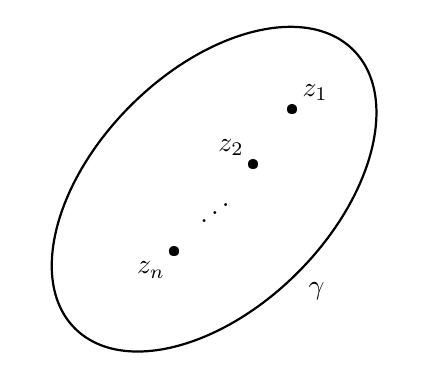
\begin{tikzpicture}
\draw[rotate around={45:(0,0)}][thick] (0,0) ellipse (2.5cm and 1.5cm);
\node at (1.3,-1.3) {$\gamma$};
\node at (1,1) {\textbullet};
\node at (1,1) [anchor=south west] {$z_1$};
\node at (0.5,0.3) {\textbullet};
\node at (0.5,0.3) [anchor=south east] {$z_2$};
\node at (-0.5,-0.8) {\textbullet};
\node at (-0.5,-0.8) [anchor=north east] {$z_n$};
\node at (0,-0.2) {$\iddots$};
\end{tikzpicture}
\qquad
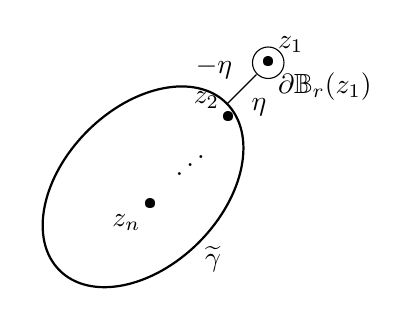
\begin{tikzpicture}
\draw[rotate around={45:(0.4,-1)}][thick] (0,0) ellipse (1.5cm and 1cm);
\node at (0.3,-1.5) {$\widetilde{\gamma}$};
\draw (1,1) circle[radius=0.2cm];
\node at (1,1) {\textbullet};
\node at (1,1) [anchor=south west] {$z_1$};
\node at (1,1) [anchor=north west] {$\partial \mathbb B_r(z_1)$};
\node at (0.5,0.3) {\textbullet};
\node at (0.5,0.3) [anchor=south east] {$z_2$};
\node at (-0.5,-0.8) {\textbullet};
\node at (-0.5,-0.8) [anchor=north east] {$z_n$};
\node at (0,-0.2) {$\iddots$};
\draw (0.85,0.85) -- (0.48,0.48) node[pos=0.5,anchor=north west]{$\eta$} node[pos=0.5,anchor=south east]{$-\eta$};
\end{tikzpicture}
\end{center}
By contour deformation theorem,
\[
\begin{aligned}
\int_{\gamma} f &= \int_{\widetilde{\gamma} \cup \eta \cup \partial \mathbb B_r(z_1) \cup (-\gamma)} f = \int_{\widetilde{\gamma}} f + \int_\eta f + \int_{\partial \mathbb B_r(z_1)} f +\int_{-\eta} f \\&= \int_{\widetilde{\gamma}} f+ \int_{\partial \mathbb B_r(z_1)} f
\end{aligned}
\tag{$\ast$}
\]
where
\[
\begin{aligned}
\int_{\partial \mathbb B_r(z_1)} f &= \sum_{k=1}^{-m} c_k \underbrace{\int_{\partial \mathbb B_r(z_1)} (z-z_1)^k \ \mathrm d z}_{2\pi i\delta_{k,-1}\text{ by Remark before Theorem 4.6.10}} + \underbrace{\int_{\partial \mathbb B_r(z_1)} \phi_1 \ \mathrm d z}_{0\text{ by Cauchy}} \\
&= 2\pi i c_{-1} = 2\pi i \text{ Res } f(z_1).
\end{aligned}
\]
Now perform induction on $\widetilde{\gamma}$ we have what's desired.
\end{proof}
\begin{example}
Calculate
\[
I=\int_{\infty}^\infty \frac{1}{x^2+a^2} \ \mathrm d x
\]
which is improper and absolutely convergent. We know this before introduction of complex analysis and we do this by computing
\[
\lim_{R\rightarrow \infty} \int_{-R}^R \frac{1}{x^2+a^2} \ \mathrm d x.
\]
\begin{itemize}
    \item[FTC:] Let $x=ay$, then
    \[
    I=\lim_{R\rightarrow \infty} \frac{1}{a} \int_{-\frac{R}{a}}^{\frac{R}{a}} \frac{1}{x^2+1} \ \mathrm d x=\left.\lim_{R\rightarrow \infty} \frac{1}{a} \arctan(x)\right|_{-\frac{R}{a}}^{\frac{R}{a}} =\frac{1}{a} \left(\frac{\pi}{2}-\left(-\frac{\pi}{2}\right) \right)=\frac{\pi}{a}.
    \]
    \item[Contour integrals:] Let $C_1^{(R)}$ be parameterised by $c_1(x)=x,\ x\in [-R,R]$ and $C_2^{(R)}$ by $c_2(x)=Re^{it}, \ x\in [0,\pi]$, and $\gamma_R := C_1 \cup C_2$.
    \begin{center}
    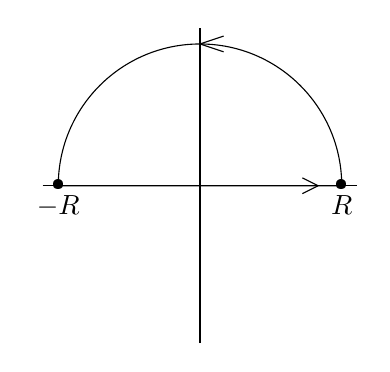
\begin{tikzpicture}
    \draw (-2,0) -- (2,0);
    \draw (0,-2) -- (0,2);
    \node at (-1.8,0) {\textbullet};
    \node at (-1.8,0) [anchor=north]{$-R$};
    \node at (1.8,0) {\textbullet};
    \node at (1.8,0) [anchor=north]{$R$};
    \draw (1.5,0) -- (1.3,0.1);
    \draw (1.5,0) -- (1.3,-0.1);
    \draw (-1.8,0) -- (1.8,0) arc(0:180:1.8) --cycle;
    \draw (0,1.8) -- (0.3,1.9);
    \draw (0,1.8) -- (0.3,1.7);
    \end{tikzpicture}
    \end{center}
    Then
    \[
    \begin{aligned}
    I&=\lim_{R\rightarrow \infty} \int_{C_1^{(R)}} \frac{1}{z^2+a^2} \ \mathrm d z \\
    &= \lim_{R\rightarrow \infty} \int_{C_1^{(R)}} \frac{1}{z^2+a^2} \ \mathrm d z+\underbrace{\int_{C_2^{(R)}} \frac{1}{z^2+a^2} \ \mathrm d z}_{\downarrow 0} \\
    &= \lim_{R\rightarrow \infty} \int_{\gamma} \frac{1}{z^2+a^2} \ \mathrm d z \\
    &= \lim_{R\rightarrow \infty} 2 \pi i \frac{1}{2ia} = \frac{\pi}{a} .
    \end{aligned}
    \]

    (Sanity check: as $R\rightarrow \infty$,
    \[
    \left| \int_{C_2^{(R)}} \frac{1}{z^2+a^2} \ \mathrm d z \right| \leq \int_{C_2^{(R)}} \frac{1}{\underbrace{|z^2+a^2|}_{\approx R^2}} \ \underbrace{|\mathrm d z|}_{R \ \mathrm d t} \leq 2 \int \frac{1}{R^2} R \ \mathrm d t \rightarrow 0.)
    \]
\end{itemize}
\end{example}

\begin{lemma}
$f,g:U\rightarrow \mathbb C$ analytic, $U$ open. Let $a\in U:g(a)=0,\ g'(a)\neq 0$ and $g(z)\neq 0 \ \forall z\neq a$. Then $\frac{f}{g}:U\backslash\{a\} \rightarrow \mathbb C$ has a first order pole. Moreover, $\text{Res }\frac{f}{g}(a) = \frac{f(a)}{g'(a)}$.
\end{lemma}
\begin{proof}
Analyticity means $\exists R_1>0:\forall z\in \mathbb B_{R_1}(a) \subset U,$
\[
g(z) = \sum_{n=1}^\infty g_n(z-a)^n \underset{g_1=g'(a)\neq 0}{=} g_1 (z-a) \underbrace{\sum_{m=1}^\infty \frac{g_m}{g_1} (z-a)^m}_{h(z)},
\]
and $f,h$ are analytic in $\mathbb B_{R_1}(a)$. Also $h(a)=1$, so $\exists R_2\in (0,R_1]:h\neq 0$ in $\mathbb B_{R_2}(a)$, so that $\frac{f}{h}$ is analytic in $\mathbb B_{R_2}(a)$. Hence $\forall z\in \mathbb B_{R_2}(a) \backslash \{a\}$,
\[
\begin{aligned}
\frac{f(z)}{g(z)} &= \frac{f(z)}{g_1(z-a)h(z)} \\
&=\frac{1}{g_1(z-a)}\left( \frac{f(a)}{h(a)}+(z-a)\phi(z) \right) \\
&= \frac{f(a)}{g'(a)} \left(\frac{1}{z-a}+\phi(z)\right),
\end{aligned}
\]
which gives what's desired.
\end{proof}

\begin{example}
We have
\[
I(k) = \int_{\mathbb R} \frac{e^{ikx}}{x^2+a^2} \ \mathrm d x, \quad a>0,\ k\in \mathbb R.
\]
Note that
\[
\left|\frac{e^{ikx}}{x^2+a^2}\right| \leq \frac{1}{x^2},
\]
so it converges absolutely. Hence, using the same $C_i^{(R)}$ and $\gamma_R$ notation, 
\[
\begin{aligned}
I(k) &= \lim_{R\rightarrow \infty} \int_{-R}^R \frac{e^{ikx}}{x^2+a^2} \ \mathrm d x \\
&=\lim_{R\rightarrow \infty} \int_{C_1^{(R)}} \frac{e^{ikz}}{z^2+a^2} \ \mathrm d z
\end{aligned}
\]
Now we know that $\frac{1}{z^2+a^2}$ goes to 0 fast enough to ensure convergence, but what about the exponential on the numerator? Note that as $z \rightarrow \infty$ along the imaginary axis, $e^{ikz}\rightarrow 0$ but as it $\rightarrow -\infty,\ e^{ikz} \rightarrow \infty$, i.e. we only have a chance of convergence if we enclose the curve in the upper half of plane (like we did in the first such example). So
\[
\begin{aligned}
&= \lim_{R\rightarrow \infty }\int_{C_1^{(R)}} \frac{e^{ikz}}{z^2+a^2} \ \mathrm d z+\int_{C_2^{(R)}} \frac{e^{ikz}}{z^2+a^2} \ \mathrm d z \\
&=\lim_{R\rightarrow \infty} \int_{\gamma_R} \frac{e^{ikz}}{z^2+a^2} \ \mathrm d z \\
\end{aligned}
\]
Let $f(z)=e^{ikz},\ g(z)=z^2+a^2$, then $g(ia)=0,\ g(z) \neq 0 \ \forall z\neq ia,\ g'(z)=2z\neq 0$. So using the lemma we know that $\frac{e^{ikz}}{z^2+a^2}$ has a first order pole at $z=ia$ and $\text{Res} =\frac{f(ia)}{g'(ia)}=\frac{e^{-ka}}{2ia}$. By Residue theorem we then have
\[
=2\pi i \frac{e^{-ka}}{2ia} = \frac{\pi e^{-ka}}{a}, \quad k\geq 0.
\]
For $k<0$, we use lower half of plane and it's symmetric, i.e. $k\mapsto I(k)$ is even (can see this by change of variables).

We conclude that
\[
I(k)=\frac{\pi e^{-|k|a}}{a},\quad \forall k\in \mathbb R.
\]

(Sanity check: as $R\rightarrow \infty$,
\[
\begin{aligned}
\left| \int_{C_2^{(R)}} \frac{e^{ikz}}{z^2+a^2} \ \mathrm d z\right| &\leq \int_0^\pi \frac{\left|e^{ikRe^{it}}\right|}{|z^2+a^2|} R \ \mathrm d t \\&\underset{R\text{ sufficiently large}}{\leq} \frac{2R}{R^2} \int_0^\pi \left|e^{ikR(\cos t+i\sin t)}\right|\ \mathrm d t \\
&= \frac{2}{R} \int_0^\pi \left| e^{ikR\cos t}\right| \left| e^{-kR\sin t}\right| \ \mathrm d t \\
&= \frac{2}{R} \int_0^\pi \left| e^{-kR\sin t}\right| \ \mathrm d t \leq \frac{2}{R} \rightarrow 0.)
\end{aligned}
\]
\end{example}

See notes for a (similar) proof of
\[
I(k) = \int_{\mathbb R} \frac{e^{ikx}}{\cosh x} \ \mathrm d x = \frac{\pi}{\cosh \frac{k\pi}{2}},\quad k\in \mathbb R.
\]
\end{document} 
